%% ut-thesis.tex -- document template for graduate theses at UofT
%DIF LATEXDIFF DIFFERENCE FILE
%DIF DEL C:\Users\David\Documents\GitHub\MASc\latex_root_before\ut-thesis.tex   Fri Dec 18 01:17:56 2015
%DIF ADD C:\Users\David\Documents\GitHub\MASc\latex_root\ut-thesis.tex          Sun Jan 10 18:56:59 2016
%%
%% Copyright (c) 1998-2012 Francois Pitt <fpitt@cs.utoronto.ca>
%% last updated at 09:43 (EDT) on Fri  1 Jun 2012
%%
%% This work may be distributed and/or modified under the conditions of
%% the LaTeX Project Public License, either version 1.3c of this license
%% or (at your option) any later version.
%% The latest version of this license is in
%%     http://www.latex-project.org/lppl.txt
%% and version 1.3c or later is part of all distributions of LaTeX
%% version 2005/12/01 or later.
%%
%% This work has the LPPL maintenance status "maintained".
%%
%% The Current Maintainer of this work is
%% Francois Pitt <fpitt@cs.utoronto.ca>.
%%
%% This work consists of the files listed in the accompanying README.

%% SUMMARY OF FEATURES:
%%
%% All environments, commands, and options provided by the `ut-thesis'
%% class will be described below, at the point where they should appear
%% in the document.  See the file `ut-thesis.cls' for more details.
%%
%% To explicitly set the pagestyle of any blank page inserted with
%% \cleardoublepage, use one of \clearemptydoublepage,
%% \clearplaindoublepage, \clearthesisdoublepage, or
%% \clearstandarddoublepage (to use the style currently in effect).
%%
%% For single-spaced quotes or quotations, use the `longquote' and
%% `longquotation' environments.


%%%%%%%%%%%%         PREAMBLE         %%%%%%%%%%%%

%%  - Default settings format a final copy (single-sided, normal
%%    margins, one-and-a-half-spaced with single-spaced notes).
%%  - For a rough copy (double-sided, normal margins, double-spaced,
%%    with the word "DRAFT" printed at each corner of every page), use
%%    the `draft' option.
%%  - The default global line spacing can be changed with one of the
%%    options `singlespaced', `onehalfspaced', or `doublespaced'.
%%  - Footnotes and marginal notes are all single-spaced by default, but
%%    can be made to have the same spacing as the rest of the document
%%    by using the option `standardspacednotes'.
%%  - The size of the margins can be changed with one of the options:
%%     . `narrowmargins' (1 1/4" left, 3/4" others),
%%     . `normalmargins' (1 1/4" left, 1" others),
%%     . `widemargins' (1 1/4" all),
%%     . `extrawidemargins' (1 1/2" all).
%%  - The pagestyle of "cleared" pages (empty pages inserted in
%%    two-sided documents to put the next page on the right-hand side)
%%    can be set with one of the options `cleardoublepagestyleempty',
%%    `cleardoublepagestyleplain', or `cleardoublepagestylestandard'.
%%  - Any other standard option for the `report' document class can be
%%    used to override the default or draft settings (such as `10pt',
%%    `11pt', `12pt'), and standard LaTeX packages can be used to
%%    further customize the layout and/or formatting of the document.

%% *** Add any desired options. ***
\documentclass{ut-thesis}

%% *** Add \usepackage declarations here. ***
%% The standard packages `geometry' and `setspace' are already loaded by
%% `ut-thesis' -- see their documentation for details of the features
%% they provide.  In particular, you may use the \geometry command here
%% to adjust the margins if none of the ut-thesis options are suitable
%% (see the `geometry' package for details).  You may also use the
%% \setstretch command to set the line spacing to a value other than
%% single, one-and-a-half, or double spaced (see the `setspace' package
%% for details).

\usepackage{amsmath}

\usepackage{graphicx}
\usepackage{caption}
\usepackage{subcaption}

\usepackage{float}
\usepackage{epstopdf}

\usepackage{hyperref}

\usepackage{multirow}

%DIF 88a88-92
\usepackage[toc,page]{appendix} %DIF > 
 %DIF > 
\usepackage{longtable} %DIF > 
 %DIF > 
 %DIF > 
%DIF -------
%%%%%%%%%%%%%%%%%%%%%%%%%%%%%%%%%%%%%%%%%%%%%%%%%%%%%%%%%%%%%%%%%%%%%%%%
%%                                                                    %%
%%                   ***   I M P O R T A N T   ***                    %%
%%                                                                    %%
%%  Fill in the following fields with the required information:       %%
%%   - \degree{...}       name of the degree obtained                 %%
%%   - \department{...}   name of the graduate department             %%
%%   - \gradyear{...}     year of graduation                          %%
%%   - \author{...}       name of the author                          %%
%%   - \title{...}        title of the thesis                         %%
%%%%%%%%%%%%%%%%%%%%%%%%%%%%%%%%%%%%%%%%%%%%%%%%%%%%%%%%%%%%%%%%%%%%%%%%

%% *** Change this example to appropriate values. ***
\degree{M.A.Sc}
\department{IBBME}
\gradyear{2015}
\author{Di Xue}
\title{Exploring the Feasibility of Prompting Daily Task Execution using \DIFaddbegin \DIFadd{the }\DIFaddend NAO Humanoid Robot \DIFdelbegin \DIFdel{to }\DIFdelend \DIFaddbegin \DIFadd{with }\DIFaddend Children with Autism Spectrum Disorder}

%% *** NOTE ***
%% Put here all other formatting commands that belong in the preamble.
%% In particular, you should put all of your \newcommand's,
%% \newenvironment's, \newtheorem's, etc. (in other words, all the
%% global definitions that you will need throughout your thesis) in a
%% separate file and use "\input{filename}" to input it here.


%% *** Adjust the following settings as desired. ***

%% List only down to subsections in the table of contents;
%% 0=chapter, 1=section, 2=subsection, 3=subsubsection, etc.
\setcounter{tocdepth}{2}

%% Make each page fill up the entire page.
\flushbottom


%%%%%%%%%%%%      MAIN  DOCUMENT      %%%%%%%%%%%%
%DIF PREAMBLE EXTENSION ADDED BY LATEXDIFF
%DIF UNDERLINE PREAMBLE %DIF PREAMBLE
\RequirePackage[normalem]{ulem} %DIF PREAMBLE
\RequirePackage{color}\definecolor{RED}{rgb}{1,0,0}\definecolor{BLUE}{rgb}{0,0,1} %DIF PREAMBLE
\providecommand{\DIFaddtex}[1]{{\protect\color{blue}\uwave{#1}}} %DIF PREAMBLE
\providecommand{\DIFdeltex}[1]{{\protect\color{red}\sout{#1}}}                      %DIF PREAMBLE
%DIF SAFE PREAMBLE %DIF PREAMBLE
\providecommand{\DIFaddbegin}{} %DIF PREAMBLE
\providecommand{\DIFaddend}{} %DIF PREAMBLE
\providecommand{\DIFdelbegin}{} %DIF PREAMBLE
\providecommand{\DIFdelend}{} %DIF PREAMBLE
%DIF FLOATSAFE PREAMBLE %DIF PREAMBLE
\providecommand{\DIFaddFL}[1]{\DIFadd{#1}} %DIF PREAMBLE
\providecommand{\DIFdelFL}[1]{\DIFdel{#1}} %DIF PREAMBLE
\providecommand{\DIFaddbeginFL}{} %DIF PREAMBLE
\providecommand{\DIFaddendFL}{} %DIF PREAMBLE
\providecommand{\DIFdelbeginFL}{} %DIF PREAMBLE
\providecommand{\DIFdelendFL}{} %DIF PREAMBLE
%DIF END PREAMBLE EXTENSION ADDED BY LATEXDIFF
%DIF PREAMBLE EXTENSION ADDED BY LATEXDIFF
%DIF HYPERREF PREAMBLE %DIF PREAMBLE
\providecommand{\DIFadd}[1]{\texorpdfstring{\DIFaddtex{#1}}{#1}} %DIF PREAMBLE
\providecommand{\DIFdel}[1]{\texorpdfstring{\DIFdeltex{#1}}{}} %DIF PREAMBLE
%DIF END PREAMBLE EXTENSION ADDED BY LATEXDIFF

\begin{document}

%% This sets the page style and numbering for preliminary sections.
\begin{preliminary}

%% This generates the title page from the information given above.
\maketitle

%% There should be NOTHING between the title page and abstract.
%% However, if your document is two-sided and you want the abstract
%% _not_ to appear on the back of the title page, then uncomment the
%% following line.
%\cleardoublepage

% This generates the abstract page, with the line spacing adjusted
% according to SGS guidelines.
\begin{abstract}
%% *** Put your Abstract here. ***
This thesis seeks to improve the state of the art prompting system, COACH, for the children with ASD population.  It investigates the prospects of using a humanoid robot, NAO, as its prompting agent through a Wizard of Oz (WoZ) pilot study, and it explores the feasibility of using a 3D camera, Kinect, to implement a Visual Focus of Attention (VFOA) tracker that enables COACH to know if the child is engaged in the activity.  The WoZ study showed promising results of the robot's ability to assist a child with ASD through hand-washing tasks.  It also suggested that parent robot joint prompting sessions as a valid method for improving child's compliance to the robot.  On the other hand, the implementation of the VFOA tracker was half completed.  Of the three component of the VFOA tracker (namely head pose tracking, eye pose tracking, object under gaze identification), only a head pose tracker and an object under gaze identifier were implemented.  The head tracker performed under normal head movements, but had limited success with the child with ASD participant during hand-washing, due to the child's rocking back and forth rapidly.  A simple Gaussian ellipsoid object location calibration method was implemented for the object under gaze identifier.
%% (At most 150 words for M.Sc. or 350 words for Ph.D.)
\end{abstract}

%% Anything placed between the abstract and table of contents will
%% appear on a separate page since the abstract ends with \newpage and
%% the table of contents starts with \clearpage.  Use \cleardoublepage
%% for anything that you want to appear on a right-hand page.

% This generates a "dedication" section, if needed
% (uncomment to have it appear in the document).
%\begin{dedication}.
% *** Put your Dedication here. ***
\section*{Dedication}
I would like to dedicate this thesis to my family -- your love, your patience, and your encouragements were the sources of my strength in this prolonged course of my study.
%\end{dedication}

%% The `dedication' and `acknowledgements' sections do not create new
%% pages so if you want the two sections to appear on separate pages,
%% you should put an explicit \newpage between them.

% This generates an "acknowledgements" section, if needed
% (uncomment to have it appear in the document).
%\begin{acknowledgements}
%% *** Put your Acknowledgements here. ***
\section*{Acknowledgments}
First, I would like to thank my supervisor, Alex Mihailidis, for his support, guidance, and kindness, through out my thesis.  In all the turning points of my thesis, he had always put my interest first.  He was patient, kind, and an expert in many research areas.  I am very grateful for knowing him as my supervisor.

I would also want to thank Tuck-Voon How, Bing Ye, and Jennifer Boger, for being the fun and resourceful people they are.  They, along with other dear members of IATSL, always made my trip to the lab fun and fruitful.

I would like to thank Jiayang Jiang for his awesome depth first search code, and Leon for teaching me the power of Latex.  I also want to thank Jason, Maria, Harry, Boyuetty, Jimverley, Stephen, Jon, Dave, and PA, for being there for me to encourage me and to spur me on when time gets hard.

Last, but not least, I am grateful for the dear Brothers and Sisters at Crosspoint Fellowship.  Without you guys, I would not have made it.

Soli Deo Gloria!
%\end{acknowledgements}


\listoffigures
\listoftables


%% This generates the Table of Contents (on a separate page).
\tableofcontents

%% This generates the List of Tables (on a separate page), if needed
%% (uncomment to have it appear in the document).
%\listoftables

%% This generates the List of Figures (on a separate page), if needed
%% (uncomment to have it appear in the document).
%\listoffigures

%% You can add commands here to generate any other material that belongs
%% in the head matter (for example, List of Plates, Index of Symbols, or
%% List of Appendices).

%% End of the preliminary sections: reset page style and numbering.
\end{preliminary}


%%%%%%%%%%%%%%%%%%%%%%%%%%%%%%%%%%%%%%%%%%%%%%%%%%%%%%%%%%%%%%%%%%%%%%%%
%%  Put your Chapters here; the easiest way to do this is to keep     %%
%%  each chapter in a separate file and `\include' all the files.     %%
%%  Each chapter file should start with "\chapter{ChapterName}".      %%
%%  Note that using `\include' instead of `\input' will make each     %%
%%  chapter start on a new page, and allow you to format only parts   %%
%%  of your thesis at a time by using `\includeonly'.                 %%
%%%%%%%%%%%%%%%%%%%%%%%%%%%%%%%%%%%%%%%%%%%%%%%%%%%%%%%%%%%%%%%%%%%%%%%%


%% *** Include chapter files here. ***

\chapter{Introduction}


\section{Motivation}

\subsection{Children with ASD and the need for ATCs}

Autism spectrum disorder (ASD) is a complex neurological and developmental condition that is characterized by impairments in social communication and the presence of repetitive behaviours and restricted interests \cite{american2013diagnostic}.  Recent research suggested that the prevalence of ASD among children aged 8 years \DIFaddbegin \DIFadd{(the peak prevalence age group)}\DIFaddend , when the broad spectrum is considered, is as high as 1:68 in the United States \cite{baoi2014prevalence}.  Although there is no federal government monitoring system currently present in Canada that provides accurate estimate of its prevalence of ASD, we know that ASD is the most common form of neurological disorder and severe developmental disability in children \cite{autism2014facts}.

Some children with ASD may have difficulty in learning self-management skills and require continuous assistance from a \DIFdelbegin \DIFdel{care-giver for }\DIFdelend \DIFaddbegin \DIFadd{caregiver to }\DIFaddend carry-out activities of daily living (ADLs).  Assistive technologies for cognition (ATCs) aim to assist, instruct, train, or educate individuals with cognitive disabilities to overcome challenges in life, including executing activities of daily living\DIFdelbegin \DIFdel{(ADL).  Especially}\DIFdelend \DIFaddbegin \DIFadd{.  In particular}\DIFaddend , autonomous or self-operated ATCs promote independence for children with ASD in need of such assistance.  Commercially available devices such as computers, video players, audio players, cellphones, etc. have all been exploited as platforms for ATCs.


\subsection{COACH and its Challenges}

The COACH (Cognitive Orthosis for Assisting with aCtivites in the Home) system, developed by Mihailidis et al., is an autonomous prompting system \cite{mihailidis2008coach}.  It uses computer vision and artificial intelligence to automatically detect user actions when executing ADLs, and prompts appropriately when a user needs assistance.  It was first developed for the dementia population, but a version appropriate to the ASD population was recently adapted and tested in a pilot study \cite{bimbrahw2012investigating}.


The system currently uses audio and video prompts using an LCD monitor screen as its primary prompting modalities.  In the pilot study, the hand-washing activity is used as an example to test the system's effectiveness because of the simplicity of its tasks as well as the washroom settings being easily controlled.  The hand-washing activity is broken into five steps, with verbal prompts being: ``turn on the water and wet your hands'', ``put soap on your hands'', ``scrub your hands'', ``rinse your hands'', ``turn off the water and dry your hands''.  At each step, if the child does not successfully execute the correct action within a time threshold, the system prompts.  The prompting consist of first displaying a still image attention grabber on screen that attempts to capture child's attention, then playing the pre-recorded audio and/or video prompts.  The video prompts are videos recorded from point-of-view (first person) perspective of a person executing the step.  If child successfully executes a step with or without prompting, the system congratulates by saying ``Good job''.  If the child \DIFdelbegin \DIFdel{doesn't }\DIFdelend \DIFaddbegin \DIFadd{does not }\DIFaddend get it right within a time threshold, the system prompts again.  This is repeated until a predetermined maximum number of times before calling over the caregiver to assist.  


The pilot study of COACH for ASD showed good acceptance by the children with ASD and their caregivers \cite{bimbrahw2012investigating}.  System effectiveness was shown in that 78\% of the hand-washing steps were completed without caregiver assistances by the children themselves, all of whom \DIFdelbegin \DIFdel{did not know how }\DIFdelend \DIFaddbegin \DIFadd{were unable }\DIFaddend to wash-hands on their own before.


The major area of improvement identified in the study was to increase the child's engagement during prompting and task execution.  Firstly, almost half of the system's prompts were ignored by the children.  Assuming that these children were able to understand the prompts, as seen by their correct actions to the not ignored prompts, their noncompliance is a reflection of their disinterest in the prompts.  Secondly, several occasions of child being distracted or disinterested to tasks were observed.


To tackle this problem, two \DIFaddbegin \DIFadd{potential }\DIFaddend approaches can be applied: 1) change the prompting modality to one that's inherently more engaging to the child (e.g. humanoid robot); 2) track the child's visual focus of attention in real-time, and issue attention grabbers when child is distracted.

\section{Roadmap}

This thesis will address how to better engage children with ASD when prompted by COACH.  It will approach the problem by incorporating a humanoid robot, NAO, and implementing algorithms to track and react to the child's gaze, in attempts to better engage children during ADL prompting sessions.


The thesis report will be broken into the following sections:


In Chapter 2, we first review the relevant literature on the established frameworks for ASD interventions, especially those that teach skills of daily living, and relate it to our prompting framework.  Next, we review research for ASD interventions that utilize technologies such as videos, computers, and robots, confirming this thesis' approach and identifying the research gap.  Also, our research direction is put into context in the Human Robot Interaction (HRI) field.  Lastly, we review state of the art research in visual focus of attention estimation, targeting key methodologies appropriate for this thesis's goal.


In Chapter 3, the research objectives and hypotheses are summarized.

In Chapter 4, the Wizard of Oz pilot study is presented.  The study setup, protocol, data collected, analysis and results are discussed in details.

In Chapter 5, the investigated algorithms for tracking a person's visual focus of attention are presented.  Specifically, the problem is broken into head pose estimation, eye pose estimation, and object identification.  The methods and evaluation for each are discussed.

In Chapter 6, we summarize and conclude the thesis.




\chapter{Literature Review}

\section{ASD Interventions}

Currently, interventions are mainly aimed to help children with ASD adjust more effectively to their environment \cite{francis2005autism}.  There are many approaches to ASD interventions, such as behavior based, pharmaceutically based, or dietary based \cite{francis2005autism}.  Also, there are interventions that focus on specific problems a child may experience, such as augmentative communication therapy, social skills teaching, sensory integration therapy \cite{francis2005autism}.  One reason for such a diverse collection of therapies to exist is because of the varying nature of ASD disabilities across individuals, making one single method not effective for the whole population, and sometimes not sufficient for an individual.  Consequently, it remains a challenge to show effectiveness of a method in a clinically significant sense, even if it is truly effective to a small sample of the population.  The most clinically tested, commonly practiced, and recommended methods are those based on the principles of Applied Behaviour Analysis \cite{foxx2008applied}.


\subsection{Applied Behaviour Analysis and \DIFdelbegin \DIFdel{Discrete Trial Training for Skill Teaching}\DIFdelend \DIFaddbegin \DIFadd{Early Intensive Behavior Intervention}\DIFaddend }
Applied Behaviour Analysis (ABA) is based on scientifically proven theories of human behaviors, and is widely used for treating inappropriate behaviors and teaching new behaviors.  Its strategies for treating inappropriate behaviors include: finding and changing antecedents to inappropriate behaviors, ignoring the behavior, or negative reinforcement through punishment \cite{foxx1982decreasing}.  Its strategies for teaching new behaviors include: giving stimuli to child to elicit a new behavior, positive reinforcement (e.g. praise), and maintenance and generalization strategies to make sure the newly learned behavior is retained across time and settings \cite{foxx1982decreasing}.  For cuing stimuli, high level of consistency is needed.  For positive reinforcement, individually selected and strategically used motivators (e.g. praise, a hug, a check mark, a favorite activity) should be given immediately after appropriate behaviors.  For maintenance and generalization strategies, prompt fading and testing across context and settings can be used.


For some children with ASD, research has shown that early ABA based intervention with \DIFdelbegin \DIFdel{persistent and intensive }\DIFdelend \DIFaddbegin \DIFadd{intensive and extensive }\DIFaddend sessions of minimum 30 hours a week for 2 years (\DIFdelbegin \DIFdel{a.k.a. }\DIFdelend \DIFaddbegin \DIFadd{also known as }\DIFaddend Early Intensive Behavioral Intervention (EIBI)) are proven to be successful for improving ASD outcomes \cite{howlin2009systematic}.  \DIFaddbegin \DIFadd{Meta analyses have been conducted to evaluate the efficacy of EIBI for children with ASD.  Three meta-analyses \mbox{%DIFAUXCMD
\cite{eldevik2009meta, reichow2009comprehensive, peters2011meta} }%DIFAUXCMD
found that, for children with ASD participating in EIBI versus those receiving other treatments or treatment as usual, an average medium to large effect size can be observed for IQ change, which may be considered clinically significant \mbox{%DIFAUXCMD
\cite{hojat2004visitor}}%DIFAUXCMD
.  Both Eldevik et al. \mbox{%DIFAUXCMD
\cite{eldevik2009meta} }%DIFAUXCMD
and Peters-Scheffer et al. \mbox{%DIFAUXCMD
\cite{peters2011meta} }%DIFAUXCMD
also found that a smaller effect size for adaptive behavior change can be observed.  However, there are large individual differences in treatment response for children with ASD and most children continue to require specialized services \mbox{%DIFAUXCMD
\cite{thill2012robot}}%DIFAUXCMD
.  All in all though, EIBI is the standard of care for children with ASD in North America \mbox{%DIFAUXCMD
\cite{keenan2014autism}}%DIFAUXCMD
.
}\DIFaddend 

\DIFdelbegin \DIFdel{Discrete Trial Training (DTT) is an ABA based method widely used for teaching }\DIFdelend \DIFaddbegin \subsection{\DIFadd{Daily Living Skill Teaching and the Discrete Trial Training}}
\DIFadd{In many children and adults with ASD, daily living skills are one of the key skills that still need to be learned through training and interventions.  In a study for adults with high functioning ASD by \mbox{%DIFAUXCMD
\cite{farley2009twenty}}%DIFAUXCMD
, they found that, among a range of variables including IQ, adaptive behavior measures (Vineland Adaptive Behavior Scales -– VABS \mbox{%DIFAUXCMD
\cite{sparrow2005vineland}}%DIFAUXCMD
) were the variables most closely and positively related to better outcome. Across the adaptive domains the ‘daily living skills’ domain was most highly associated with better outcome of quality of life.
}

\DIFadd{There are three major cognitive theories developed that attempt to explain the underlying mechanics of the difficulties experienced by individuals with ASD: Theory of Mind deficit, executive dysfunctioning, and weak central coherence \mbox{%DIFAUXCMD
\cite{rajendran2007cognitive}}%DIFAUXCMD
.  The Theory of Mind deficit explains some individuals with ASD's inability to create an image of an agent's mental states (including one's own), thus the inability to infer what others think, believe, and desire, consequently to predict their behaviors.  Executive dysfunctioning explains some individuals with ASD's impairments in several higher-level capacities necessary for planning and monitoring of behaviors, set shifting, inhibiting automatic actions, and holding information in working memory.  Weak central coherence explains some individuals with ASD's cognitive style of local or detail-focused processing, leading to missing more global processing of information in context and for meaning.  These cognitive impairments in individuals with ASD are the underlying factors that cause some individuals to have difficulties learning and executing activities of daily living.  One approach to address this is through cognitive function trainings that focus on learning isolated cognitive skills that the individual lacks.  It has been found, however, that improvements in adaptive behaviors may not automatically result in improvements in cognitive skills \mbox{%DIFAUXCMD
\cite{chin2000teaching, teunisse2007cognitieve}}%DIFAUXCMD
.  Thus, instead of targeting the cognitive skills, which might not generalize to adaptive behaviors, the more direct approach would be to target the behaviors themselves, through interventions such as those based on the ABA framework.
}

\DIFadd{Discrete trial teaching (DTT) \mbox{%DIFAUXCMD
\cite{howard2005comparison}}%DIFAUXCMD
, incidental teaching (IT) \mbox{%DIFAUXCMD
\cite{mcgee1986extension}}%DIFAUXCMD
, and pivotal response training (PRT) \mbox{%DIFAUXCMD
\cite{koegel2003teaching} }%DIFAUXCMD
are interventions effectively used in adaptive skill building in }\DIFaddend children with ASD \DIFdelbegin \DIFdel{new }\DIFdelend \DIFaddbegin \DIFadd{and are based on ABA methodology \mbox{%DIFAUXCMD
\cite{palmen2013behavioral}}%DIFAUXCMD
.  DTT focuses on specific targeted }\DIFaddend behaviors, and \DIFdelbegin \DIFdel{particularly useful in teaching skills }\DIFdelend \DIFaddbegin \DIFadd{relies on intensive and repetitive trainings with appropriate and immediate reinforcements.  IT focuses on teaching the child through natural means, emphasizing on having the child initiate learning opportunities.  For example, the therapist may hide one of the shoes of the child before it is time to go outside, thus creating an opportunity for the child to request verbally the missing shoe.  PRT philosophy also emphasizes naturalistic teaching.  Instead of focusing on individual behaviors, it targets ``pivotal'' areas of the child's development, such as motivations, response to multiple cues, self-management, and initiation of social interactions.  By targeting these key pivotal areas for improvement, broad area improvements can be seen in sociability, communication, behavior, and academic skill building.
}

\DIFadd{Reviewing these methods, DTT is the most appropriate for teaching skills for a single activity }\DIFaddend of daily living\DIFdelbegin \DIFdel{\mbox{%DIFAUXCMD
\cite{smith2001discrete}}%DIFAUXCMD
}\DIFdelend \DIFaddbegin \DIFadd{, such as teaching hand-washing}\DIFaddend .  Many studies have shown effectiveness of EIBI using DTT, as reviewed by Case-Smith et al. \cite{case2008evidence}: The original study of DTT, by Lovaas, compared two groups of 19 young children with ASD, one receiving 40 hours per week of intensive DTT and the other receiving 10 hours or less of similar training, and showed improved IQ for the former after 2 years of intervention \cite{lovaas1987behavioral}.  There are many studies that confirmed these findings.  For one, in a more recent study, Cohen et al. compared two groups of 21 children with ASD, one receiving EIBI for one year and moved to less intensive services after, the other group receiving community-based services only, and showed higher IQ, language comprehension, and adaptive behavior for the former group by the end of 3 years \cite{cohen2006early}.  In addition, \DIFaddbegin \DIFadd{the DTT method is reproducible by nonprofessionals, as well.  }\DIFaddend Sallows et al. showed that parents who are taught proper implementation of DTT produced similar results with children with ASD as those produced by trained therapists after 4 years \cite{sallows2005intensive}.

\subsubsection{Implementation Details of DTT}
\DIFdelbegin \DIFdel{There }\DIFdelend \DIFaddbegin \DIFadd{In summary, there }\DIFaddend are five steps to \DIFdelbegin \DIFdel{a }\DIFdelend DTT \cite{bogin2010steps}:
\begin{enumerate}
	\item Grabbing the child's attention
	\item Discriminative stimulus: must be simple, clear, and concise, and wording must be consistent
	\item Child's response: stop incorrect response by instructing again immediately or provide prompts
	\item Prompt to aid the child if no response or wrong: this has the advantage of helping him quickly move through trials and avoid boredom and frustration.  Always use least intrusive prompt that ensures correct response.  Fade prompts to promote maintenance of effect and prevent dependence on intervention.  Types of prompts include: verbal, gesture, modeling, visual, physical.
	\item Reinforcement: given immediately after correct responses, tailored individually, always pair with verbal praise.
\end{enumerate}

%DIF < AM: I would like to see this section developed a bit more, including looking at more details on why this approach is important to follow, some more examples of clinical studies that have proven its efficacy, and then how this may map to the COACH and the importance of doing so.
\DIFdelbegin %DIFDELCMD < 

%DIFDELCMD < %%%
%DIF < why DTT is important to follow:
%DIF < 	- examples of clinical studies that proves its efficacy
%DIF < 	- how does it map to COACH
%DIF < 	- why is it important to map it to COACH
%DIFDELCMD < 

%DIFDELCMD < %%%
\subsection{\DIFdel{Discussion}}
%DIFAUXCMD
\addtocounter{subsection}{-1}%DIFAUXCMD
%DIFDELCMD < \label{sec:DTTDiscussion}
%DIFDELCMD < %%%
\DIFdel{To promote consistency and effectiveness, the implementations of ATCs for assisting children with ASD with daily living tasks should also follow the ABA framework, and model after the DTT steps.  Apparently, an ATC acts as either a substitute or a complement to the caregiver in guiding the child with ASD through ADLs in the home / community settings.  The goals for a successful ATC for children with ASD are two fold: one, to guide the child through an ADL without dependence on the caregiver; and two, to train the child to perform the steps of the ADL with fading dependence on the ATC. The development of ATC can take advantage of the principles of incorporating DTT.  This approach would potentially provide therapeutic interventions in the home / community settings.  In fact, this is exactly what COACH aims to achieve in its prompting design.  The following are the steps of how COACH prompts:
}%DIFDELCMD < \begin{enumerate}
%DIFDELCMD < 	\item %%%
\DIFdel{Attention Grabber
	}%DIFDELCMD < \item %%%
\DIFdel{Verbal Instruction
	}%DIFDELCMD < \item %%%
\DIFdel{Video Prompt
	}%DIFDELCMD < \item %%%
\DIFdel{Child's Response
	}%DIFDELCMD < \item %%%
\DIFdel{Verbal Reward
}%DIFDELCMD < \end{enumerate}
%DIFDELCMD < 

%DIFDELCMD < %%%
\DIFdelend \section{Assistive Technology for ASD}
Assistive Technology (AT) refers to ``any device or piece of equipment that facilitates teaching new skills, augments existing skills, or otherwise reduces the impact of disability on daily functioning'' for individuals with disabilities \cite{lang2014assistive}.  Defined by Individuals with Disabilities Education Act Amendments of 1997, an AT is ``any item, piece of equipment, or product system ... that is used to increase, maintain, or improve functional capabilities of individuals with disabilities'' [Part A, Sec. 602 (1)].  The ATs used in the context of cognitive disabilities, such as those from dementias, stroke, mental illness, acquired brain injury and intellectual disability, are termed Assistive Technologies for Cognition (ATC) \cite{frank2004assistive}.  In this section, we will review the literatures of ATCs specifically for assisting individuals with ASD.

Two major reviews have been identified in this field: Lang et al.'s \cite{lang2014assistive} and Goldsmith et al.'s \cite{goldsmith2004use}.  In these reviews, roughly 60 studies were identified that targeted various abilities (or the lacking of abilities) of individuals with ASD using various forms of technologies as interventions.  The various targeted abilities can be divided into three groups: (a) communication skills, (b) social and emotional skills, and (c) daily living and other adaptive skills \cite{lang2014assistive}.  The various forms of technologies used in the interventions can be divided into auditory prompting, speech generating device, script training, tactile prompting, picture exchange communication systems, video modeling, and computer-based interventions.  In this section, we will focus on summarizing the results of the studies grouped by the targeted abilities, and critique the effectiveness and limitations of various forms of technologies used for each targeted ability group and draw parallel of the technologies used across targeted ability groups.

\subsection{Assistive Technology for Communication Skills}
Individuals with ASD experience varying degrees of disabilities in communication skills \cite{howlin2003outcome}.  Individuals with autism may experience limited speaking abilities or may fail to develop speech at all \cite{weitz1997aac}, while individuals with Asperger's syndrome often develop speech skills, but may fail to communicate well due to limited topics of interest, inabilities to recognize social cues, and anxieties related to social situations \cite{scheuermann2002teaching}.  In addition, individuals with ASD may develop speech stereotypies such as echolalia (i.e. repeating other's words verbatim) \cite{sigafoos2007assessing}.

Various ATCs have been developed to help individuals with ASD cope with or improve their communication skills.  Two major forms of technologies that help individuals with ASD cope are Picture Exchange Communication System (PECS) and Speech Generating Devices (SGD) \DIFdelbegin \DIFdel{a.k.a. }\DIFdelend \DIFaddbegin \DIFadd{(also known as }\DIFaddend Voice Output Communication Aid (VOCA)\DIFaddbegin \DIFadd{)}\DIFaddend .  Both PECS and SGD fall under the category of aided Augmentative and Alternative Communication (AAC) \cite{sigafoos2001conditional}, which relies on using visual cues such as symbols and pictures as a way for individuals with ASD to select the desired content of communication, since their visual processing abilities are thought to be often well developed (\cite{mirenda2001autism, shane2012applying}).

PECS is very simple technology wise\DIFdelbegin \DIFdel{, it }\DIFdelend \DIFaddbegin \DIFadd{.  It }\DIFaddend involves the person with ASD to communicate by giving the other person a picture or symbol card representing their communicative intent \cite{bondy1994picture}.  There are four meta-analysis reviews investigating the effectiveness of using PECS as a communication system for people with ASD \cite{ganz2012meta, ganz2012metab, sulzer2009picture, tincani2010quantitative}.  PECS was identified as a promising intervention, and resulted in improved communication outcomes, and its effect size and that of the SGD's are among the greatest effect sizes compared against other AAC interventions.  PECS were also associated with increased speech produced for individuals already producing speech and increased social approaching in some individuals with ASD \cite{lang2014assistive}.  The mechanism of which PECS increases speech is not well understood \cite{preston2009review}, but hypotheses have been raised regarding how the caregiver's speech were encouraged during the PECS interactions with the user, and that served as a model for speech for the user \cite{yoder2006randomized}.

SGD is more advanced technology wise\DIFdelbegin \DIFdel{, it }\DIFdelend \DIFaddbegin \DIFadd{.  It }\DIFaddend involves a portable device which can playback pre-recorded or synthesized speech messages when the person with ASD presses the panels or switches on the device.  Pictures or symbols are used to indicate what content is being played as speech.  Typical message includes requesting, commenting, and greeting, ``for example, a picture of a favorite toy may be used to indicate that the message 'May I have my toy please?' will be played if the corresponding panel on the SGD is activated'' \cite{lang2014assistive}.  There are four meta-analysis reviews investigating the effectiveness of using SGD as a communication system for people with ASD \cite{van2010communication, van2011assessing, ganz2012metab, ganz2013moderation}.  SGD was also identified as a viable intervention, it improved communication outcomes, and its effect size (and that of PECS') is greater than other AAC interventions (even had greater effect size than PECS for problem behavior treatment), and was the preferred device by some individuals with ASD over the PECS \cite{lang2014assistive}.  The increased speech was likely due to correct speech modeling during SGD's speech playback \cite{schlosser2008effects}.

Comparing between PECS and SGD, we see that both works as an effective alternative to individuals with ASD who are unable to self-produce speech.  Interestingly, both devices are reported to increase self-produced speech from some individuals using them, and were believed to be the effects of correct speech modeling (directly from the device in SGD's case and from the caregiver in PECS' case).  In addition, the SGD holds advantage over PECS in that more complex messages can be delivered and communication attempts may be more easily understood by most communication partners \cite{mirenda2001autism}.  Also, SGD devices can take forms as an iPhone or iPod (the software can be loaded as an app), and the ubiquity of such handheld devices among typically developing peers may reduce the stigmatization of using SGD for communication \cite{kagohara2013using}.

Besides coping, there are also ATCs that teach and improve communication skills.  The only form of technology used for teaching communication skills currently found in literature is Computer Based Interventions (CBI).  CBI describes any software that runs on a computer aiming to improve certain skills for individuals with ASD through an interactive curriculum in a virtual learning environment \cite{lang2014assistive}.  The use of CBI for improving communication skils is reviewed by Ramdoss et al. \cite{ramdoss2011use}.  In the review, 10 studies with total of 70 participants (children 14 years or younger diagnosed with autism) were identified.  No studies with adults or individuals with Asperger's syndrome were included in the review.  The studies' aims can be divided into three groups: ones focusing on associating vocabulary words with pictures \cite{moore2000brief, hetzroni2005logos}; ones focusing on receptive identification and speech production of the vocabulary words \cite{heimann1995increasing, bernard1999enhancing, bosseler2003development, coleman2005using, massaro2006read}; and ones focusing on verbal initiation and relevance of speech during social settings \cite{parsons1993effect, simpson2004embedded, hetzroni2004effects}.  The softwares involved were either commercially available (e.g. Alpha program \cite{abledata2010alpha}, Baldi/Timo \cite{2005team}, HyperStudio \cite{mackiev2010welcome}, AbleData \cite{abledata2010alpha}, PowerPoint \cite{1997microsoft}, Speechviewer \cite{synapse2010the}) or were programmed by the research team.  All of the studies reported positive effects of using the CBI.  It's interesting to note that the softwares used share similarities in that they all implement some form of reinforcement schedules.  And for the latter two groups of studies, they all involved visually engaging graphics (e.g. a computer generated head in Baldi or animated color graphics of words in Alpha program), and relate the user to the vocabulary speech by synchronizing the graphics with the speech.


\subsection{Assistive Technology for Social Skills}
Lack of social skills is one of the diagnostic criteria for both autistic disorder and Asperger's syndrome \cite{spitzer1980diagnostic}.  Some symptoms include (a) lack of appropriate eye contact, (b) inability to develop peer relationships, (c) failure to initiate or maintain joint attention, and (d) lack of social and/or emotional reciprocity \cite{rao2008social}.

There are many ATCs focusing on either coping with (i.e. teaching is not the primary objective) and\DIFaddbegin \DIFadd{/}\DIFaddend or improving social skills for individuals with ASD.  For the former, one of the ATCs identified by the review by Goldsmith et al. \DIFdelbegin \DIFdel{was }\DIFdelend \DIFaddbegin \DIFadd{were }\DIFaddend Tactile Prompting devices \cite{goldsmith2004use}.  Tactile Prompting devices are portable devices individuals with ASD can carry and vibrate during the social interaction scenarios in attempt to promote self initiation to social interactions or promote responses to peer initiations.  The tactile prompting devices were either programmed to vibrate periodically or were controlled remotely by the researcher.  The studies identified in the review reported increased social interaction initiations for individuals with ASD including verbal initiations \cite{shabani2002increasing, taylor1998teaching} and handing communication cards \cite{taylor2004teaching}.

In addition to Tactile Prompting devices, another ATC has also been used for coping -- Script Training.  Script Training involves modeling a certain social interaction through a script and the individual with ASD is given a written copy of the script or hears it from a recording or a person reading it \cite{stevenson2000social}.  Not only does the script contain verbal speeches of interactions, the script may also contain prompts for the individual to follow, such as approach a potential conversation partner, initiate conversation, turn to the speaking person, maintain eye contact, wait until the person finishes talking, etc. \cite{wichnick2010effect}.  As an example, Wichnick et al. used a voice over recording device that plays back pre-recorded audio scripts when children with ASD and peers exchanged toys \cite{wichnick2010effect}.  Through continuous use, an improvement of response to peer initiation was observed, and the number of novel responses increased as scripts were faded.

Instead of coping with lack of social skills, there are ATCs that aim to teach and improve social skills.  By pooling the studies reviewed by Goldsmith et al. \cite{goldsmith2004use}, Lang et al. \cite{lang2014assistive}, Ramdoss et al. \cite{ramdoss2012computer}, and  Shukla-Mehta et al. \cite{shukla2009evaluating}, we have found two forms of ATCs that teach social skills to individuals with ASD: Computer Based Interventions and Video Modeling.

The CBI studies mainly focused on two groups of outcomes: The first group deals with promoting social responsiveness and interactive play, teaching social conflict resolution, and anger and anxiety management.  The second group deals with recognition of facial features, expressions, and interpreting emotions from faces, body language, and voices.  The results using CBI for the first group were positive, provide preliminary evidence that CBI technology-based interventions may be effective for some children with ASD, while the results for the second group were mixed but mainly positive \cite{ramdoss2012computer}.  Also, studies were unable to prove that CBI is better than face-to-face-training course in teaching social skills.  Lastly, there were very little evidence on the generalization of the social skills learned from CBI.  Possibly the reason why the second group had mixed results was because of the complexity of the skills involved is higher than those in group one, or the lack of such skills required in group two is more severe in individuals with ASD.  Instead of teaching, maybe in-vivo CBI solutions that aims for coping need to be developed to fill this gap.

Video Modeling is the other form of ATCs that \DIFdelbegin \DIFdel{teaches }\DIFdelend \DIFaddbegin \DIFadd{teach }\DIFaddend social skills.  As reviewed by Shukla-Mehta et al. \cite{shukla2009evaluating}, video modeling techniques can be divided into video modeling (VM), video self-modeling (VSM), and point-of-view video modeling (PVM).  VM involves the individual with ASD being asked to watch a video before instructed to practice certain target skill.  In the video, the target skill is modeled by an adult or a peer.  \DIFdelbegin \DIFdel{During watching of }\DIFdelend \DIFaddbegin \DIFadd{While watching }\DIFaddend the video, the instructor prompts and provides reinforcers to the individual with ASD for attending relevant stimuli in the video.  It is expected that the individual would imitate the model's behaviors shown in the video when practicing the targeted skills immediately after \cite{bellini2007meta, graetz2006show}.  The individual would either watch a short video of some discrete target behaviors before practicing it in its entirety or watch a video clip of one step, practice the step, then watch the next clip and practice the next step.  It is found that for discrete target behaviors, a 3-5 min video is considered adequate for individuals with ASD \cite{buggey2005video}.  VSM is similar to VM except that the model in the video performing the targeted skills with the desired behaviors is the individual with ASD him/herself \cite{hitchcock2003video}.  This is based on the assumption that no one is a better model similar in age, gender, race, and other characteristics than oneself \cite{bandura1969principles, buggey1999training}.  VSM often involves showing videos of the individuals with ASD themselves successfully performing an exemplary behavior that is already in their repertoire or one they are learning.  This may mean carefully cutting out the scenes of undesired behaviors of the individual when making the videos, and could prove challenging for a novel skill the individual has not acquired yet.  PVM is similar to VM and VSM except that the video is shot from the visual perspective of the model as opposed to shot from a third person's perspective \cite{hine2006using}.  The purpose of PVM is that, when the individuals see the video, they see a smooth transition of what is expected of them from beginning to end of the routine.  Such techniques would ``promote visual comprehension and increase familiarity with materials and settings, and reduce task anxiety and inappropriate behaviors'' \cite{shukla2009evaluating}.

Shukla-Mehta et al.'s review included 26 studies, out of which the majority used VM, \DIFdelbegin \DIFdel{4 }\DIFdelend \DIFaddbegin \DIFadd{four }\DIFaddend studies used VSM, and only \DIFdelbegin \DIFdel{2 }\DIFdelend \DIFaddbegin \DIFadd{two }\DIFaddend studies used PVM \cite{shukla2009evaluating}.  The studies using VM focused on modeling verbal social initiations (e.g. compliments, social greetings, scripted and unscripted verbalization for pretend play etc.) as well as appropriate play behaviors (e.g. perspective taking, reciprocal play, sharing, eye contact, smiling, etc.).  The VSM and PVM studies also focused on similar goals as VM, with PVM also including a study that aimed to reduce severe problem behaviors (e.g. crying, screaming, dropping on the floor).  All of the studies reported positive outcomes, with some studies needing more than simply showing the videos to the individuals (instructional prompts, reinforcers and error correction were also implemented) to ensure acquisition, maintenance, and generalization of target skills.  It was also noted that the individual with ASD's skills in attending, imitation, visual processing and comprehension, matching-to-sample, and spatial ability influence the outcomes, thus planning the amount of content and length of video appropriate for the individual depends on these variables.  Lastly, there were no sufficient evidence suggesting the type of model (self, peer, familiar or unfamiliar adult) had an influence on VM's effectiveness.

\subsection{Assistive Technology for Daily Living and Other Adaptive Skills}
For an individual to function independently and successfully, daily living and other adaptively skills such as self-care (e.g. hand-washing), organization (e.g. time management), and community (e.g. grocery shopping) skills are crucial \cite{liss2001predictors}.  Some individuals with ASD, however, have a hard time acquiring such crucial skills and need to rely on the assistances of caregivers \cite{smith2012developmental}.

ATCs have been used to assist individuals with ASD in the skills outlined above.  There is not a comprehensive literature review published on ATCs for daily living skills, however, Lang et al.'s review summarized nine studies in this field \cite{lang2014assistive}.  Almost all of the nine studies involved either a Computer Based Intervention (CBI) \cite{hutcherson2004computer}, a form of Video Modeling (VM \cite{rosenberg2010evaluating}, PVM \cite{bereznak2012video, shipley2002teaching, sigafoos2007evaluation, sigafoos2005computer, van2010comparison}), or a combination of the two called Computer Based Video Instructions (CBVI) \cite{ayres2009acquisition, mechling2010computer}.  The targeted tasks in the studies included preparing food, setting up table, grocery shopping, bus stop request, hand-washing, mailing letters, caring for pets, dish washing, and clothes folding.

CBI based ATCs and VM based ATCs both showed positive results in assisting individuals (diverse in age range) with ASD through the tasks.  CBI was particularly successful in creating a virtual environment in which individuals with ASD can focus on the controlled stimulus teaching them the task.  CBI is also good in giving consistent and immediate positive reinforcements automatically.  CBI focuses on teaching the skills needed to perform the target task in-vitro, and does not assist the performance in-vivo.  Thus, generalization of the skills learned from the virtual environment needs to be tested in the real life settings.  All CBI studies reviewed here involved some form of in-vivo generalization testing, and positive results were reported.

As effective as CBI, if not better, is video modeling (VM) interventions.  Of all the VM interventions, PVM was the most popular because it enables individuals with ASD with a first-person-view to better relate the materials presented in the video to the task at hand. However, positive results were reported for other VMs as well, giving evidence that video modeling in general is an effective way of teaching individuals with ASD the daily tasks required. There are no studies done using VSM, since the skills involved are novel and it is hard to produce videos of the individual performing an unlearned novel skill. From here on, we will not distinguish the different forms of VM. VM ATCs can be used as a in-vitro teaching tool, just like CBI, by letting the individual with ASD view the entirety of the video before performing the task. Studies involving in-vitro video modeling often needs verbal prompts and positive reinforcement in terms of verbal praises, toys or food rewards to motivate individual's concentration towards the training video. Although this method shows positive outcome, many of the studies reviewed here involved in-vivo video modeling.  This involves splitting the task into subtasks and display video for one subtask, then allow the individual to perform that subtask, after which it displays the video for the next subtask, and so on. This has the advantage of managing the complexity of each subtask needing to be performed as well as assisting the individual with ASD to plan which subtask to perform next.  Another common practice in VM ATCs was that verbal instructions were delivered as a voice over in the video.  The verbal instructions were short phrases that either describe the subtask being performed in the video or describe the stimulus in the video the individual should pay attention to.  Not only can the VM based ATCs be used in-vivo, individuals with ASD can be taught to use them by themselves, enabling their independence in real world scenarios.  IPods and laptops have both been used in studies that demonstrated the ability of individuals with ASD to self prompt, by playing and pausing the model videos or by pressing the next button, at each subtask.  Such self prompting skills were taught by having the teacher first model the operation of the ATC in person or through video modeling, using an exemplar task.  Then after the training sessions, the teacher starts the individuals with ASD on the actual task, and encourages them to seek assistance from the ATC when they encountered problems they do not know how to solve.

Marrying the advantages of CBI and VM, CBVI shares the ability to create virtual training environment and deliver accurate reinforcement schedule like CBI, and is able to effectively train individuals with ASD the skills involved in the task like VM.  Positive results were reported by two studies.  In one study by Ayres et al., a computer program taught individuals with ASD preparing meals.  In this study, a modified system of least prompts (SLP) arrangement was used, with the prompting hierarchy being, from least to most intrusive: 1. independent (no prompts), 2. verbal prompt (short phrase of what to do), 3. video prompt (video modeling the subtask), 4. partial physical prompt (the computer shows visually where to click in order to execute the subtask, but requires the user to click it), 5. full physical prompt (the computer clicks for the user) \cite{ayres2009acquisition}.  In this arrangement, the individual with ASD is given a chance to complete each subtask without prompts, if not successful, a prompt with increasing level of intrusion is given, until the subtask is done either by the individual or by the computer.  This prompt hierarchy was useful in implementing prompt fading for the goal of promoting maintenance and independence.  Note however that the prompt hierarchy is easily implemented in-vitro since the computer has full knowledge of how well along the task the user is doing in the virtual environment it created.  However, for in-vivo prompting hierarchy, either a human or an artificial intelligence is needed for understanding user states.

Of all the studies reviewed (CBI, VM, and CBVI), there are a couple of common themes in their methodologies.  First, all the studies that are systematic and complete in their method tested for the effectiveness of ATC in the following areas: acquisition of skill with ATC, maintenance of skill without ATC, maintenance of skill over time, and generalization of skill across settings.  Of course, not all the studies need to show effectiveness of the ATC in all four areas, since this may be difficult for some studies (e.g. pilot studies that do not aim to have follow ups 3 months after) and inappropriate for others (e.g. acquisition without prompts were not the aims for some ATCs).  Second, individuals often need positive reinforcement during in-vivo task execution.  There are always either some sort of encouragement from the instructor (e.g. verbal praise) or a real motivating reason for the individual to succeed in the task (e.g. eat the popcorns made).

\DIFaddbegin \subsection{\DIFadd{ABA Based ATCs}}
\DIFadd{As mentioned in the previous section, ABA based interventions showed clinical significance in improving IQ for at least some children with ASD, and showed promising outcomes for improving their adaptive skills as well.  It is natural to think we can capitalize the successes of ABA principals into ATC designs.  So far, most of the ATCs discussed above were designed as tools used by the individual with ASD or by the therapist / caregiver.  The ABA framework may include the use of such ATCs by the choice and design of the therapist, but the implementation of the ABA methods is outside of these ATCs' design scope.  This is why most of the literatures in ATCs for ASD interventions do not discuss the use of the ABA framework explicitly in its device design section.  However, when the ATC serves both the role of a tool as well as the agent facilitating the intervention session, such as in the case of CBI devices capable of context aware autonomous prompting, the implementation of ABA elements such as priming, discriminative stimuli, prompt, reinforcement schedule, prompt fading, become integral to the device design.
}

\DIFadd{There are currently four softwares that have publications that explicitly state the implementations of the ABA framework in their designs, namely the DT Trainer \mbox{%DIFAUXCMD
\cite{ashton2001applications}}%DIFAUXCMD
, the DTTAce \mbox{%DIFAUXCMD
\cite{picardo2014towards}}%DIFAUXCMD
, the Cosmo's Learning System (CLS) \mbox{%DIFAUXCMD
\cite{lathan2007using}}%DIFAUXCMD
, and the TeachTown: Basic \mbox{%DIFAUXCMD
\cite{whalen2010efficacy}}%DIFAUXCMD
.  The DT Trainer programs cover three functions: labeling (matching simple object labels to functional information associated with images), sounds (matching sounds and their corresponding item pictures), and questions (answering how an item and a function are associated, e.g. cut with scissors, eat with a spoon).  The DTTAce software runs on a touchscreen table, where the child with ASD can interact with virtual objects jointly with the therapist to learn about the concept of colors.  CLS takes the form of a virtual world in which the main character, Cosmo, motivates the child with ASD to solve various problems.  The problems focus on identification of color, shape, number, directions, prepositions, and written words as well as sequencing skills and discrimination of relative size and amount.  The TeachTown: Basic is also a virtual world, in which the child with ASD chooses a part of the town to visit, and solves training problems unique to that part of the town.  The problems included exercises in language, cognitive, auditory processing, and social skills.  All four softwares implemented some form of positive reinforcements, and also implemented automatic user progress tracking.
}

\DIFadd{The publications for DT Trainer and DTTAce only presented the design concepts, but did not present any evaluation studies investigating their efficacies.  The CLS, on the other hand, has been evaluated on six children with ASD in single subject design.  All subjects demonstrated improvements in all content areas except color identification. Children learning prepositions and direction improved an average of 20\%.  Similar gains were made in written word reading. Children learning relative size/amount improved but had difficulty understanding the concept ‘same’.  For TeachTown: Basic, numerous studies have been published evaluating efficacies, validating reinforcements, and investigating maintenance.  The most recent and extensive study evaluated efficacy in forty seven children with ASD in a between-subject design (twenty two in treatment group).  Compared to the students in the control group, the treatment group showed more improvement overall on language and cognitive outcome measures.
}


\DIFaddend \subsection{Discussion}
\label{Sec:AT4ASDDiscussion}
From reviewing the ATC \DIFdelbegin \DIFdel{literatures }\DIFdelend \DIFaddbegin \DIFadd{literature }\DIFaddend for assisting individuals with ASD, we found several forms of technologies that are proven to work.  They differ in complexity technology wise, however, they share similarities in that they either teach the target skill in-vitro or help to cope with the lack of skills in-vivo.  In addition, some common techniques found across the different forms of technologies are: the ATC engages individuals with ASD visually, gives them direct instructions, shows them the exact model behavior expected of them, provides them a consistent and simplified environment to practice the skills, and motivate them through positive reinforcement.  The different forms of prompting modalities include audio prompting, tactile prompting, and visual prompting.

We saw that, for modeling techniques such as script training and video modeling, instructions and reinforcements were needed during the modeling session as well as during the task execution session.  The instructions served as a way to help the individual with ASD to focus on certain stimuli necessary to learn the skill during modeling, and to help the individual to stay on task during task execution.  The reinforcements served as motivations for the individual to stay engaged and motivated during the trials.

CBI stood out as a technology that is very versatile and proved to be useful for training many skill areas.  In general, it is speculated that the success of CBI was due to the following reasons: First, a computer is consistent and predictable and is believed to be the preferred instructional delivery modality for individuals with ASD who prefer routines \cite{ramdoss2011use}.  This puts CBI advantageous to caregiver based interventions.  Second, a computer provides a virtual learning environment that reduces distractions and controls for autism-specific learning characteristics (e.g. stimulus overselectivity) \cite{lovaas1979stimulus}.  This puts CBI advantageous to some ATCs that aim for in-vivo learning.  Lastly, a computer can accurately implement complex reinforcement schedules and prompt fading, promoting learning and generalization \cite{ramdoss2011useb}.  This puts CBI advantageous over video modeling, since CBI can incorporate video modeling as part of the curriculum, while providing reinforcement and prompt fading.

CBI maybe successful in teaching skills to individual with ASD in-vitro,  but the generalizability of skills learned through computer intervention in-vivo is questionable.  Since the ultimate goal is for the individual to perform the skill learned in-vivo, another strategy is to simply use ATCs in-vivo for teaching the skill.  An important focus of research in this strategy is how to get the individual with ASD to be self-sufficient with the ATC in-vivo.  There were three ways: train the individual with ASD to self operate the ATC, remote control the ATC, and have an automated ATC.  The second method does not provide true functional independence, since a remote operator is still needed.  But this method can be viewed as an intermediate prototype before full automation of the ATC, and is useful in testing the automated ATC without realizing its automation.  Thus, we will mainly compare the first and third method here.  The first method involves teaching the individual with ASD to self operate the ATC.  This has been shown to be feasible for several forms of ATCs (tactile prompting, verbal prompting, and video prompting).  However, it requires certain fine motor skills from the individual for manipulating the ATC's controls, and requires certain level of executive functioning to learn to seek help from the ATC.  The alternative is to use a fully automated ATC.  One basic form of automated ATC was to periodically play a certain prompt during task execution.  This strategy is simple to implement, but is often not as effective as if the prompt was delivered contingent to the context.  However, in order to do this, a computer program is needed that understands and tracks the context the user is in, and delivers the appropriate prompt when user needs it.  Such automation is feasible for CBI ATCs, since the virtual environment is fully controlled by the computer program.  However, for in-vivo ATCs to realize this automation, some form of artificial intelligence (AI) is needed that understands the real-life environment.  Up to date, the only ATC that fills this gap is COACH \cite{bimbrahw2012investigating}, which uses computer vision and AI to understand the current hand-washing task the user is undergoing and delivers prompts when the user does not execute a task within a preset time period, and delivers positive reinforcement when the user executes a task correctly.

Relating to the issue of promoting functional independence of individual with ASD using in-vivo ATCs, a common strategy adopted is prompt fading, where the prompts used were slowly tuned down over time in its specificity.  This has the effect of decreasing the individual with ASD's reliance on the prompts, in hope that one day the individual could execute the tasks without the ATC.  This in-vivo prompt fading strategy were shown to be successful in promoting generalization of a learned skill, and should be implemented for all in-vivo ATCs.  COACH also adheres to this requirement as well, implementing a hierarchy of prompts (video modeling, picture prompts, verbal prompts), and decreases the prompt level over time as user's skills progress.

In conclusion, we see that various forms of ATCs have been proven useful for assisting individuals with ASD, and COACH fills an unique gap by delivering fully automated prompts and reinforcements in-vivo.  It has the advantage of in-vivo ATCs, easing in the learning of a new skill in-vivo and ensuring generalization.  It also retains the advantage of in-vitro ATCs (e.g. CBI), providing consistent and accurate reinforcement schedules.  Thus, the approach that COACH offers is founded in good grounds.  This thesis aims to further improve COACH by exploring novel interaction modalities that better engage individuals with ASD, all the while preserving its in-vivo and CBI advantages.
\DIFaddbegin 

\label{sec:DTTDiscussion}
\DIFadd{As mentioned earlier, when implementing a prompting system that serves the role of the agent facilitating the daily living skill training session, one must consider implementing ABA principals as part of its design.  In fact, this is exactly what COACH aims to achieve.  The following are the steps of how COACH currently prompts, which follows the DTT method:
}\begin{enumerate}
	\item \DIFadd{Attention Grabber
	}\item \DIFadd{Verbal Instruction
	}\item \DIFadd{Video Prompt
	}\item \DIFadd{Child's Response
	}\item \DIFadd{Verbal Reward
}\end{enumerate}
\DIFadd{The improvements to COACH contributed by this thesis will also adhere to the DTT method.
}

\DIFaddend \section{Human Robot Interactions (HRI)}

HRI is a recent field of research focusing on natural and efficient interactions between humans and robots.  It is a multidisciplinary field with contributions from human computer interactions (HCI), artificial intelligence, robotics, design, social sciences, etc.  The study of HRI is important for designers of robot behaviors, especially if one pursuits a framework of user centered design, where user experience is given as much value as functionalities. 


\subsection{Socially Interactive Robotics (SIR)}
SIR is first defined by Fong et al. as robots for the main purpose of interacting with users without physical contact \cite{fong2003survey}.  The application domains where SIR are desirable are: robot as mediator of human-human interactions, robot as representations of humans, robot as companions to human, robot as modeling tool for researchers studying embodied social behaviors.  The kinds of social interactions SIR could simulate include: artificial emotions, speech, facial expression, body language and gesture.  We will refer to these as different modes of human-robot interactions through out this thesis.


\subsection{The Issue of Embodiment}
One major issue in the study of SIR (and that of HIR in general) is the issue of embodiment, i.e. what effects does the robot's physical presence have on its interactions with humans.  Ziemke \cite{ziemke2001disentangling} defined four levels of embodiment from least to most:
\begin{enumerate}
	\item \textbf{Structural coupling}: the presence (does not have to be physical) of the agent can influence a human's state
	\item \textbf{Physical embodiment}: the agent has a physical body
	\item \textbf{Organismoid embodiment}: the agent's physical body is organism-like
	\item \textbf{Organismic embodiment}: except the agent's organism-like body is of autopoietic, living systems
\end{enumerate}


The impact of embodiment in SIR is significant, as argued by Mataric \cite{mataric2005role}.  Because humans irrepressibly attribute human-like characteristics to embodied agents that are similar to them, the factors influencing the embodiment of the robot will impact significantly the engagement of the human in HRI.


Similar intuition is explored by Young et al \cite{young2011evaluating}.  As Young et al. pointed out, because the robot has an embodied presence in close proximity to the user, it has a greater influence than the disembodied counterpart on the user physically, emotionally, and socially. Thus, factors in embodiment has a large influence on how the user perceives the robot's identity and their relationship.  Young et al. provided a three level perspective on how to analyze these factors in embodiment in context of HRI:
\begin{enumerate}
	\item \textbf{Intrinsic level}: static factors regarding the appearance of the robot set the initial emotional response from the user.  For example, a cute looking robot animal may create instant affinity from children towards the robot.  Static qualities of the robot's voice and motion (e.g. amplitude, smoothness, speed, etc.) fall under this level, too.  In addition, factors in this level contribute to the role user perceives the robot to be in.  For example, a humanoid is better than an animal looking robot as a supervisor or mentor.

	\item \textbf{Behaviour level}: dynamic factors regarding the facial expressions, voice intonations, motion gestures and gaze, etc. modulate emotional responses from the user and interactions between user and robot.  In addition, these factors contribute to the robot's perceived role as well.

	\item \textbf{Role level}: the goal of the robot, and the planning and decision making of the robot's behaviors to achieve that goal (along with factors from previous two levels), determines the perceived role of the robot.  The user may treat the robot as a supervisor, mentor, companion, cooperative peer, slave, tool, etc. \cite{goodrich2007human}.
\end{enumerate}


\subsection{Socially Assistive Robotics (SAR)}
Feil-Seifer and Mataric defined SAR as the intersection of socially interactive robotics (SIR) and assistive robotics (AR) \cite{feil2005defining}.  In the past, AR has been mainly been used to describe robots that assisted people with physical disabilities through physical contacts.  But SAR arises from the need for robots to assist people with cognitive disabilities without using physical contacts.  In this context, SAR assumes an expert (mentor / coach / supervisor / teacher / assistance) role, and prompts the user through executions of tasks.  Feil-Seifer and Mataric pointed out that SAR has two (possibly conflicting) goals –- engaging the user to HRI and engaging the user to executing tasks.  SAR needs careful designing to satisfy both the social interaction goal and the assistive goal.  However, on a deeper level, the SIR goal is serving the AR goal in that, better social interactions would cause better user engagement during the co-operative activity, and yield better user compliance to prompts and ultimately better task performance.


Wainer et al. conducted studies along this line of hypothesis, evaluating user engagement through self-reflective survey and evaluating task performance through optimality of move during the task of solving a Towers of Hanoi puzzle \cite{wainer2007embodiment}.  They tested the difference between embodied robot versus its remote presence and its simulated virtual avatar (both disembodied versions are displayed on a computer screen).  They have found that people prefer interacting with the embodied robot and reported it being more helpful and watchful than the other two disembodied counter parts.  However, there were no significant improvements in task performances from using the embodied robot over the disembodied versions.


\subsection{Discussion}
This lack of impact on task performance in Wainer et al.'s study may be due to the learning effect when solving the puzzle and the novelty factor of using the robot.  Also, the use of such SAR on the clinical population and on clinically relevant tasks may yield a better result because of greater need for user engagement and user compliance in that context.  For our thesis, we will investigate the impact of a prompting agent embodied as a humanoid robot on the clinical population of children with ASD in the task of hand-washing, where user's lack of compliance to prompts and engagement in task executions are observed problems.  One thing to note is, we cannot conduct self-reflective surveys due to the nature of the children with ASD population.  Therefore, we will rely on objective measures for user engagement such as verbal responses and physical behaviors (proximity, posture, eye gaze) \cite{mataric2005role} as well as subjective observations from the parents and the researcher.



\section{Robots in ASD Interventions}


A recent popular area of research for ASD interventions is robot-based interventions.  This is due to recent advancements in HRI research, as outlined in the previous section, as well as successes shown in studies in using robot in the clinical settings for children with ASD.  Clinical studies of this approach is reviewed by Diehl et al., and the studies have been categorized based on the study purposes \cite{diehl2012clinical}.


\subsection{General Response to Robots}
Several studies have investigated how individuals with ASD interact with robots in general, and have compared it with human counterparts.  Dautenhahn et al. showed that some individuals with ASD prefer interactive robots compared to passive toys \cite{dautenhahn2004towards}.  Robins et al. showed that ASD individuals prefer robot-like characteristics over human-like in social interactions \cite{robins2006does}.  Pierno et al. found that children with ASD respond faster to robotic movement than human movement \cite{pierno2008robotic}.


\subsection{Eliciting Pro-Social Behaviours}
Robins et al. showed that children showed increased social interaction behaviors towards the robot in some areas such as proximity to robot, eye gaze, touch, imitation \cite{robins2005robotic}.  Feil-Seifer et al. suggested that social behaviors of children with ASD increased when the robot is acting contingently to child's actions, as opposed to randomly \cite{feil2009toward}.  Ravindra et al. showed the potential for robot and ASD individuals to share joint attention towards objects \cite{ravindra2009therapeutic}.


\subsection{Modeling, Teaching, or Practicing a Skill and Providing Reinforcements}
Not many studies have been conducted for skill execution training, since most studies have focused on addressing the social aspects of ASD interventions.  One preliminary study by Duquette et al. examined the use of humanoid robot to help children with ASD practice imitation behaviors \cite{duquette2008exploring}.  Positive reinforcements were also given through the robot raising arms and saying ``Happy!'' when the child successfully imitated the robot.  In their study result, children with ASD showed more interest to the robot when the robot is mediating the training session, as compared to their interest during human mediated sessions.  Also, in the robot's presence, fewer repetitive behaviors with their favourite toy were observed.


\subsection{Discussion}
Of particular interest to this thesis is Ravindra et al.'s study \cite{ravindra2009therapeutic}, in which they implemented a detector of object of visual focus of attention.  Using head pose plus eye pose estimations, and mixture of Gaussian modeling of object locations, they were able to detect with 75\% accuracy the object of the child's gaze (i.e. visual focus of attention).  The detector is then used as a feedback to the robot's prompting system for instructing the child to interact with objects through verbal command and gesture prompt (robot points and gazes at the object).


Even though their study's purpose is to train children with ASD with joint attention skills, their study showed the plausibility of utilizing similar techniques for prompting the child to pay attention to or interact with any objects of interest.  Particularly in our thesis, we aim to implement two aspects of their techniques to guide children with ASD through hand-washing:
\begin{itemize}
	\item \textbf{Robot gesture prompt}: point and gaze at an object while instructing the child how to interact with the object.
	\item \textbf{Robot behavior loop}: loop consisting of attention grabber (AG), prompt, reinforcement if instruction successfully followed, loops from AG again if failure (illustrated in Figure \ref{fig:ravindra2009therapeutic}).
\end{itemize}
\begin{figure} [h]
	\centering
	\includegraphics[width=0.6\textwidth]{./img/ravindra2009therapeutic.png}
	\caption{Robot behavior loop used by Ravindra et al. \cite{ravindra2009therapeutic}}
	\label{fig:ravindra2009therapeutic}
\end{figure}

In Diehl et al.'s review, it was pointed out that studies in skill training would benefit from integrating robots into the ABA framework \cite{diehl2012clinical}.  As discussed in Section \ref{sec:DTTDiscussion}, this is what we propose any skill training ATC system should do, similar to COACH.  Thus including a robot into our COACH system would fill this research gap.


In all, from these studies, we see a great potential for increasing the attention and engagement level of the ASD child if we incorporate a humanoid robot into our COACH system.  The robot may serve as an attention grabber as well as a prompting agent.

\section{Visual Focus of Attention Estimation}
%Some kind of intro is needed here on why it is important to review the literature in this area.  It doesn't come across anywhere that this is a key technique you are using and why.
One of the key initiators of communication is joint attention, and grabbing and maintaining the visual attention of the user is an important functionality in the design of socially assistive robots \cite{torta2012can}.  In the context of this thesis, a robot is used to teach and practice hand-washing skills with children with ASD.  In its interaction with the child, successfully grabbing and maintaining the child's attention during the activity will ensure the child receives the prompts as the robot delivers it, and thus increasing the chance that the child complies to the prompts.  To this end, the robot behaviors need to be engaging to the child.  But more importantly, the robot behaviors should be contingent to the child's behaviors.  If the child is not paying attention, for example, an attention grabber (e.g. robot waves hand and call out to the child) would serve as a communication opener before delivering the prompt.  This enables the system to adhere to the DTT prompting framework mentioned in Section \ref{sec:DTTDiscussion}.  Because of this, the robotic system needs to be able to detect the visual attention of the child in real-time.

\subsection{Visual Focus of Attention and Gaze}
If we define Visual Focus of Attention (VFOA) as what a person is looking at, then given that we know what and where objects of interest are in the scene, the problem for VFOA estimation becomes estimating the direction and depth of a person's visual focus (i.e., gaze).
%Are there not standard definitions of these things that you can use and reference?

For consistency, we define the 3 degrees of freedom (DOFs) of head pose as pan, tilt, and roll (see Figure \ref{fig:murphy2009head}), with reference direction for pan and tilt being frontal direction of the head facing the camera.  We define 2 DOFs of eye pose as pan and tilt similar to head pose, with reference direction for pan and tilt same as head pose.
\begin{figure} [h]
	\centering
	\includegraphics[width=0.6\textwidth]{./img/murphy2009head.png}
	\caption{DOFs of Head Pose, adapted from \cite{murphy2009head}}
	\label{fig:murphy2009head}
\end{figure}


Then, gaze direction is given by the accumulated rotation of average eye pose on head pose \cite{funes2013person}, gaze depth is given by the intersection of the left and right eye pose directions.  Therefore, the problem can be divided into head pose estimation and eye pose estimation.


\subsection{Head Pose Estimation}
There has been extensive research for head pose estimation for a single image frame, or head tracking for a video stream of images.  As reviewed by Murphy-Chutorian et al., the following categories of methods have been identified: appearance templates, detector arrays, nonlinear regression methods, manifold embedding methods, geometric methods, and flexible models \cite{murphy2009head}.


\subsubsection{Appearance Templates and Detector Arrays Methods}
Appearance templates methods and detector arrays methods are mainly for estimating discrete / coarse head pose.  For our task of identifying the object of interest under visual focus of attention, we do not know a priori where and how close to each other the objects are.  Therefore, only continuous fine pose estimation methods are of interest and are reviewed in this thesis.


\subsubsection{Nonlinear Regression Methods}
Using a machine learning approach, a direct mapping from the cropped head image to pose can be learned.  Because such mapping is highly nonlinear, nonlinear regression methods, such as Support Vector Regressors (SVR) \cite{li2000support} and Neural Networks (Multilayer Perceptron (MLP) \cite{voit2008head}, and Locally Linear Map (LLM) \cite{kruger2002gabor} have been applied in this context as supervised learning, using head images as inputs and head poses as ground truths.

Although neural networks are among the most popular and accurate methods in head pose estimation, they are prone to errors from poor head localizations.  And since, in our application, we cannot restrict user to remain in the center of the camera's field of view at all times, we need to either seek out a separate localization method for cropping the head, or seek a head tracker that doesn't have this problem.  Using face detectors for localization is one solution, but it only works for near frontal poses, bottlenecking the head tracker's operating range.


\subsubsection{Manifold Embedding Methods}
Manifold embedding methods learn a projection from high dimensional image space to some low dimensional space.  The methods are unsupervised learning methods that only require head images and not pose ground truth labels.  Promising techniques include: Isometric feature mapping (Isomap) \cite{raytchev2004head}, Locally Linear Embedding (LLE) \cite{roweis2000nonlinear}, and Laplacian Eigenmaps (LE) \cite{belkin2003laplacian}.


However, due to the fact that they ignore pose labels, the projected low dimensional space may not be capturing appearance variations due to head pose alone, but may also include appearance variations due to identity, lighting, etc., making pose prediction inaccurate.  Although there are work around techniques in the manifold embedding methods to tackle the appearance variations due to identity, more systematic ways to deal with it are seen in the following two methods: geometric methods and flexible model methods.


\subsubsection{Geometric Methods}
Geometric methods use person independent facial features (e.g. corners of eyes and mouth, tip of nose, etc.) to predict head pose.  The relative locations of these features are exploited with geometrical assumptions of a person's face such as parallelism, symmetry and proportion \cite{wang2007enhancement}.


A major caveat of these methods is that their accuracy relies on accuracy of features tracking.  For our scenario of a child washing hands at the sink, where a moderate resolution camera captures a mid-range field of view, features are not guaranteed to be tracked with ease.  Thus, it is better to select head pose estimation methods that do not require local features tracking.


\subsubsection{Flexible Model Methods}
Flexible model methods explicitly models the identity as well as pose of a person's face.  Given a representation of the face, flexible models for shape and texture can be constructed using PCA from a face database to represent the directions in which the face most likely (naturally) deforms.  Using this model, a new face image can be fitted through optimizing both an identity parameter and a pose parameter.  This way, pose can be extracted independent of identity.


There are two popular and related flexible model methods: Active Appearance Model (AAM) and 3D Morphable Model (3DMM).  They differ in the following ways:

\paragraph{Face Representation}
Although both models use triangulated mesh representations of the face, AAM uses a 2D representation while 3DMM uses a 3D one.  Also, AAM uses a sparse mesh with vertices at local features while 3DMM uses a dense mesh with vertices at the pixel level.  These make AAM more computationally efficient, but on the other hand 3DMM more robust to low resolution image, partial occlusions, lighting variations, and large head rotations.


\paragraph{Face Fitting}
Because AAM operates in 2D, fitting simultaneously the pose as well as the identity parameters requires us to recover a 3D model of the face using a structure-from-motion algorithm and then use the 3D model's weak perspective projection to constrain 2D fitting \cite{xiao2004real}.  3DMM fitting is less convoluted if using a RGB-D camera (e.g. the Kinect camera).  The pose and identity can be fit simultaneously using a non-rigid iterative closest point algorithm (Optimal Step Non-rigid ICP) \cite{paysan20093d}.

\subsubsection{Kinect Fusion}
Very similar to 3DMM, the Kinect Fusion algorithm developed by Microsoft also can be used to build a 3D head model, and track its orientation through ICP \cite{newcombe2011kinectfusion}.  The main difference between the two algorithms lies in that 3DMM uses the optimal step non-rigid ICP, which uses a parameterized model of a person's face generated by doing PCA of a face model database.  On the other hand, the head model generation from Kinect Fusion simply rely on building a point cloud of the head, thus its model is not parameterized.  Besides this head model generation step that is different, everything else used in head pose tracking are the same -- rigid ICP alignment.  However, since 3DMM focuses on modeling the face while Kinect Fusion is capable of modeling the whole head, Kinect Fusion may perform better in tracking extreme head poses where the face is largely obstructed.  3DMM, on the other hand, can be tolerant of dynamic expressions on a person's face \cite{amberg2008expression}, while Kinect Fusion may yield poorer tracking when the head model deforms.

\subsection{Eye Pose Estimation}
Eye pose estimation for a single image frame, or gaze tracking for video stream of images, have also been extensively researched.  Here we present results from a recent review by Hansen et al. \cite{hansen2010eye}.  Eye pose estimation methods can be categorized as shape-based, feature-based, and appearance-based:


\subsubsection{Shape-Based Methods}
Shape-based methods are seeking to contour fit the shapes of iris, pupil, eye, etc.  Some examples include: a simple model of ellipse fitting the shape of iris or pupil region, proposed by Valenti et al. \cite{valenti2008accurate}; a complex model of deformable template fitting the eye and pupil shape, proposed by Colombo et al. \cite{colombo1999real}.


\subsubsection{Feature-Based Shape Methods}
Feature-based shape methods seek eye structure localization through identifying a set of distinctive local features.  One can use features directly in the intensity image, with features found for example in limbus, pupil, cornea reflections, eye corners, etc.  An example for this is the neural network method by Reinders et al. \cite{reinders1996locating}.  One can also use features in a filter response of the image, for example seen in the method of A Sirohey et al. \cite{sirohey2001eye}.


Both the shape-based and feature-based methods are inaccurate for moderate resolution mid-range field of view images -- they often require a close up view of an eye.  The problem with large field of view containing not only the eye regions is two fold.  First, lower resolution for the eye regions are available, making the above methods less accurate.  Second, without a proper localization of the eyes, false positives arise.  Methods combining head pose and eye pose estimation is an effective way to combat the false positives in a large field of view as well as dealing with large head poses.  It improves accuracy through the two estimators constraining each other in localizations \cite{valenti2012combining}.  However, a better way, as seen in the head pose tracking section of the literature review, is to use appearance-based methods.


\subsubsection{Appearance-Based Methods}
Another approach to deal with moderate resolution mid-field images is through appearance-based methods.  One can directly model the mapping from eye appearance to eye pose, seen by the neural network method of Baluja et al. \cite{baluja1994non}.  However, direct modeling requires large number of training images, the collection of which is a tedious process.  One way to reduce number of training images needed is through template matching with local linear interpolation.  An example of this is the Adaptive Linear Regression (ALR) method of Lu et al. \cite{lu2011inferring}.


The major caveat with these appearance-based methods, as similarly to head pose estimation, is the inability to separate appearance variations in identity from pose.  One way to tackle this is through keeping a bank of personal models, seen in Mora et al. \cite{funes2013person}.  A new person's eye images can then be represented by a linear combination of exemplar eye images from people in the bank using ALR.  Then, to ease computational cost of ALR, we only keep the top few models that have their exemplar eye images used most often, decreasing the search space during ALR's optimization step.


\subsection{Using RGB-D Camera for Gaze Estimation}
The works of Mora et al. are good fits to our application \cite{funes2012gaze, funes2013person}.  Specifically, their approach uses the 3DMM head pose estimation together with ALR eye pose estimation.  One thing to note is that the commercial grade RGB-D camera, Kinect, is used.  Although 3DMM works with 2D camera as well, getting a direct sensor input on the depth information is advantageous in this context because it avoids inferring the 3D structure from 2D images, reducing inaccuracies and computations. Also, it enables 3DMM to estimate pose through shape alone, ignoring texture fitting altogether, reducing computations and increasing robustness to lighting.


\subsection{Discussion}
From the reviews, we see that Kinect Fusion and ALR are ideal for our application.  They yield many advantages:  Firstly, usage of appearance-based methods means we are moderate resolution mid-field scenario ready.  Secondly, only a simple calibration step is needed to generate the head model for Kinect Fusion and a bank of people's exemplar eye images are needed for ALR.  For the children with ASD population, having relatively simple calibration step that does not require the child to behave in a certain way is very useful.  Next, once the person's head model is generated, pose can be fitted without fitting identity, reducing computations.  Lastly, the head image can be restored to the frontal head pose and a consistent frontal eye region cropped out, making eye pose estimation robust to large head poses.



\chapter{Research Objectives}

\section{Overall Goal and Approach}
Our overall goal is to increase a child with ASD's engagement level during COACH prompting for hand-washing tasks, and thus improving prompt \DIFdelbegin \DIFdel{compliance }\DIFdelend \DIFaddbegin \DIFadd{complying }\DIFaddend and task completion rate.  Our approach is:
\begin{enumerate}
	\item to incorporate a half body humanoid robot, NAO T14 (see Figure \ref{fig:HalfBodyNAO}) by Aldebaran Robotics, into the current COACH setup, capable of delivering verbal and gesture prompts and attention grabbers

	\item to automatically track the VFOA of the child so that the robot can call out \DIFaddbegin \DIFadd{the }\DIFaddend child's name with a waving gesture or blink its LEDs for getting child's attention if the child is not looking at the robot before prompting

\end{enumerate}
\begin{figure} [h]
	\centering
	\includegraphics[width=0.6\textwidth]{./img/nao_t14_schema}
	\caption{The Half-Body Version of Humanoid Robot NAO}
	\label{fig:HalfBodyNAO}
\end{figure}


\section{Central Hypothesis}
We hypothesize that the incorporation of a humanoid robot prompting agent, such as NAO T14, would sufficiently capture and maintain children with ASD's attention during prompting and keep them engaged during task execution, so that high prompt compliance rates and task completion rates would be achieved when assisting them through ADLs such as hand-washing.


\section{Specific Objectives}

\paragraph{Our objectives are:}
\begin{enumerate}
	\item To investigate if a prompting system using NAO is able to guide child with ASD through hand-washing, and identify factors for improvement

	\item To explore the different modes of interactions between NAO and child when prompting hand-washing steps using a Wizard of Oz setup, focusing on verbal, gestures, and gaze for the modes of interactions

	\item To \DIFaddbegin \DIFadd{explore how to }\DIFaddend implement a real-time algorithm for tracking child's VFOA
\end{enumerate}



\paragraph{Our hypotheses are:}

%	\item Child has greater general engagement level when interacting with NAO than with the parent.


%general engagement level:
%# of times child smiles
%# of times child murmurs
%# of times distracted

%visual focus correct:
%look at prompting agent given prompt rate
%look at step attempted given attempt rate

%prompt compliance and task completion:
%compliance rate
%# of prompts till compliance
%time duration till compliance
%task completion rate
%# of prompts till finished step before prompt
%time duration of extended steps
%number of presses for soap
%# of times requiring physical intervention

%independence:
%# of times child start step before prompt
%# of times child finishes step before prompt

%what measures for survey? just qualitative report? any processing / analysis needed before reporting?

\begin{enumerate}
	\item The humanoid robot, NAO, is able to independently assist child with ASD through hand-washing, and child exhibits greater engagement level, higher prompt \DIFdelbegin \DIFdel{compliance }\DIFdelend \DIFaddbegin \DIFadd{complying }\DIFaddend rate, and better task completion when prompted by NAO than by parent.

	\item Gestural, gaze, and verbal are the essential modes of interactions present in the hand-washing prompting scenario between child with ASD and the prompting agent NAO.

\DIFdelbegin %DIFDELCMD < \item %%%
\DIFdel{Using 3DMM and ALR for estimating head pose and eye pose, and using the Kinect camera, a classification rate of more than 80\% is achieved for estimating child's VFOA on NAO, monitor screen, soap, towel, tap region, hands, and idling.
	}\DIFdelend %DIF > 	\item Using 3DMM and ALR for estimating head pose and eye pose, and using the Kinect camera, a classification rate of more than 80\% is achieved for estimating child's VFOA on NAO, monitor screen, soap, towel, tap region, hands, and idling.

\end{enumerate}

\chapter{The Wizard of Oz Pilot Case Study}

%What are we trying to find out? Why are they important?
%	- is there a difference in child's response to parent prompt vs robot prompt?
%		- visual attention
%		- compliance
%		- task performance


%WoZ experiment design
%	- what is WoZ? why do we use this scheme?
%	- experiment design, why use this design
%	- short blurb of the experiment
%Recruitment
%	- inclusion criteria
%	- method of recruitment, target sample size
%NAO
%	- overall description, capabilities
%	- general design decisions for
%		- verbal prompts
%		- gesture prompts
%Protocol and Setup
%	- experiment / equipment setup for data collection
%	- protocol
%	- video data to be collected
%	- survey to be collected
%	- ethics considerations
%Video annotation protocol
%Measures
%Analysis and results:
%	- participants recruited
%	- video data collected
%	- video analysis method
%	- video analysis results
%	- inter-rater agreement analysis and results
%	- survey data collected
%	- survey analysis method and results
%Discussion:
%	- results interpretations
%	- interpretation limitations
%	- original objectives achieved or not
%	- future outlook

\section{Research Design and Strategy}
One major objective of this thesis is to investigate the impacts that using a humanoid prompting agent has on the visual attention, prompt compliance, and task performance of children with ASD during hand-washing activities.  This is the first research of its kind in the field of humanoid robot prompting agent guiding children with ASD through an activity of daily living.  Therefore, it is wise to begin with a pilot study, the purpose of which is to show plausibility of the key underlying assumptions of our hypotheses, to create design recommendations of the robot for future studies, and to probe what questions are important to be answered later in a more rigorous randomized control trial.  For these reasons, the pilot study should be exploratory in nature, having a flexible \DIFdelbegin \DIFdel{experiment }\DIFdelend \DIFaddbegin \DIFadd{experimental }\DIFaddend design, and a relatively low experiment setup cost.  A Wizard of Oz \DIFdelbegin \DIFdel{experiment }\DIFdelend \DIFaddbegin \DIFadd{experimental }\DIFaddend design in a case study format is appropriate.

\subsection{Wizard of Oz \DIFdelbegin \DIFdel{Experiment }\DIFdelend \DIFaddbegin \DIFadd{Experimental }\DIFaddend Design}
The Wizard of Oz (WoZ) is an \DIFdelbegin \DIFdel{experiment }\DIFdelend \DIFaddbegin \DIFadd{experimental }\DIFaddend design widely used in Human Computer Interaction (HCI) and Human Robot Interaction (HRI) research.  In a typical WoZ study, there is an interactive agent that is not yet fully autonomous, and is remotely controlled by a human operator (i.e. the ``wizard''), and this fact is concealed from the user being tested until after the study.  The wizard may control one or many parts of the agent, such as speech recognition and understanding, affect recognition, dialog management, utterance and gesture generation and so on \cite{bhargava2013demonstration}.  The advantage of a WoZ study is that it does not require a large amount of work spent in implementing the artificial intelligence (AI) behind the agent before testing it in a study -- it is mocked up by the wizard remote controlling the agent.  This is great for testing hypotheses early on in the design loop, enabling us to obtain feedbacks from users, learn, and iterate through design cycles faster.  Of course, care needs to be taken to ensure the mocked up part of the AI is implementable in the near future, since the real purpose of the mock up is to have an early knowledge of the real design constraints, not trying to provide a less constrained solution.

The characteristics of a WoZ study fits our pilot study requirements, where we want to learn early the important design questions regarding building an effective ADL prompting robotic agent for the children with ASD population.  Thus, we have conducted a WoZ study in which a humanoid robot whose motions and speech were preprogrammed, but the decision and timing of their executions were controlled remotely by the researcher.  The researcher, acting as the wizard, is mocking up the computer vision algorithms that understand the child with ASD's actions, the speech recognition algorithms that recognize the child's verbal interactions, and the AI decision making algorithms that decide what prompts to deliver and when to deliver them.

During each WoZ study trial, the child with ASD was asked to complete the hand-washing activity in the washroom with the supervision of one of his/her parents, with the help of the NAO robot, or with the help of both the parent and the robot. The researcher \DIFdelbegin \DIFdel{, }\DIFdelend and the parent \DIFdelbegin \DIFdel{if the child was to be assisted only by the robot, }\DIFdelend were in an adjacent room out of the child's view to observe his/her hand-washing activity.  However, the parent could enter the washroom if the child needed physical assistance to complete a step. A controlling interface running on a laptop, connected wireless to the robot, was used by the researcher to remotely control the robot, as well as to monitor the progress and responses of the child through the video feeds of the cameras installed in the washroom.

\subsection{Case Study Format}
The WoZ study was conducted, analyzed, and reported in a case study format.  A case study is defined by Yin in a two fold definition: ``a case study is an empirical inquiry that investigates a contemporary phenomenon in depth and within its real-life context'' and its result ``relies on multiple sources of evidence, with data needing to converge in a triangulating fashion'' \cite{yin2013case}.  The case study format is widely used in human robot interaction research for children with ASD \cite{kozima2005interactive, robins2004robot, robins2009isolation}.  This is because the case study format can be exploratory as opposed to evaluative in nature, employing both quantitative and qualitative data analyses, and dealing with a small number of subjects \cite{yin2013case}.  For research in human robot interactions for children with ASD, these qualities of a case study are advantageous.  Firstly, HRI research in children with ASD is a relatively novel field, not having a sound theoretical foundation, and it is yet to be systematically established which hypotheses are important to test.  Thus, it is more effective in filling research gaps by conducting pilot studies that focus on generating important hypotheses in an exploratory manner rather than conducting those that focus on testing hypotheses not soundly founded.  Secondly, since a major aspects of HRI research (similar to HCI research) addresses understanding the whys and hows of user decision making, qualitative data including researcher observations, interviews, focus groups, surveys, etc. are of as much importance as quantitative metrics, if not more, during the early stages of research.  Lastly, since each child with ASD is unique and vastly different from the rest of the spectrum, starting with pilot studies that focus on only a few cases / subjects in depth and iteratively move up the sample size to eventually aim to generalize across a population is preferential.

The case study format applies well to this thesis.  Our WoZ pilot study falls under HRI research for children with ASD, and our aim of generating important hypotheses and robot design recommendations in an exploratory manner makes the case study format highly suitable.  This does mean that comparing to typical quantitative pilot studies (e.g. Bimbrahw et al. \cite{bimbrahw2012investigating}), we needed to restrict to a smaller sample size, to iteratively generate and test hypotheses during data collection, and to report the results in a more descriptive manner.

\subsection{Combining Qualitative and Quantitative Analyses}
Qualitative and quantitative analyses in this thesis' case study play complimentary roles with each other.  From a result description point of view, there are certain aspects of the study best summarized by stating qualitatively the themes or trends observed, while other aspects of the study demand accounting of metrics whose trends (or lack of trends) are presented by graphical plots.  The decisions of which results are presented qualitatively and which quantitatively will be discussed more in Section \ref{Sec:DataAnalysisAndResults} -- Data Analysis and Results.  From a hypotheses generation and validation point of view, qualitative analyses provide the intuitive understanding and interpretation of our study results, while quantitative analyses provide further investigation and validation to the hypotheses generated by the qualitative analyses.  Through observations and discussions of the child with ASD's behaviors in response to robot and parent prompts, qualitative analyses may identify important trends and themes that can be validated using quantitative analyses.  The choice of metrics used in quantitative analyses are, in turn, dependent on the qualitative observation results.  This is coherent to the triangulation approach that qualitative research employs, which assumes that the internal validity of a research is strengthened when the use of multiple sources of data, multiple methods, multiple investigators, or multiple theories confirms the same findings \cite{merriam2014qualitative}.  Quantitative analyses, then, can be the ``one more method'' that confirms and strengthens the validity of the findings from the qualitative research.

One challenge of conducting qualitative and quantitative analyses alongside in this complimentary manner within a study is that, for qualitative research, data analysis is conducted during data collection, and data collection method is revised iteratively with ongoing analysis \cite{merriam2014qualitative}.  For example, if analysis reveals that a certain device should be improved or a certain data collection protocol should be changed, data collection may take a turn in this new direction.  This may potentially create problems for quantitative analysis if it shares with qualitative analysis the same pool of data collected.  For the data collected using methods that are changing, grouping them would be not rigorous if the changes may significantly affect our outcome, but not grouping them would make the sample size very small for each group.  For this thesis, however, this may be a compromise we are willing to accept for the pilot study, since the validity of our results rest not solely on quantitative analyses.  It is planned for future studies to conduct a statistically significant quantitative research for rigorously validating the hypotheses and design recommendations generated by this thesis.

\subsection{Case Selection and Sample Selection}
\label{sec:CaseSelectionAndSampleSelection}
When conducting a case study, selecting the right case and sampling in it the data to focus on are essential for bounding the scope of the study and producing results of significance.  The case selection and the sampling within the case are essentially two layers of the same process called sample selection \cite{merriam2014qualitative}.  Merriam \cite{merriam2014qualitative} listed several sample selection methods.  Of them, the ones most relevant to a case study are typical sampling, unique sampling, maximum variation sampling, and theoretical sampling. As Merriam defines them:
\begin{itemize}
	\item \textbf{Typical Sampling} chooses samples that are the ``average person, situation, or instance of the phenomenon of interest''
	\item \textbf{Unique Sampling} focuses on ``unique, atypical, perhaps rare attributes or occurrences of the phenomenon of interest''
	\item \textbf{Maximum Variation Sampling} explores extreme variations of the phenomenon of interest, sometimes even involving ``a deliberate hunt for negative or disconfirming variations''
	\item \textbf{Theoretical Sampling}  is ``an ongoing sample selection process'' that ``begins the same way as purposeful sampling'' (purposeful sampling includes the three sampling methods above), ``but the total sample is not selected ahead of time'' but is decided iteratively as results from data analysis roll out
\end{itemize}

In our WoZ pilot case study's context, case selection was the process of setting inclusion criteria for recruiting a subpopulation of the children with ASD, and sample selection within the selected case was deciding the robot and parent prompting protocols that are used to guide our participant through the hand-washing trials.  Case selection is be discussed in more detail in Section \ref{sec:Recruitment} - Recruitment.  Sample selection is discussed in more detail in Section \ref{sec:StudyProtocol} - Study Protocol.



\section{Recruitment}
\label{sec:Recruitment}
Since children with ASD are a diverse population with each child unique and vastly different from one another, the subpopulation from which we recruit from directly influences our study results and focus.  This is the process of case selection.  Since the aim of our study is to form important hypotheses about children with ASD that aid in future iterations of the robot prompting design, focusing on the typical use case would be most beneficial at the pilot study stage.  One way to ensure this is through sampling for the typical user that our robot is designed for.  This would be children with ASD, not adults nor any one without a diagnosis of ASD.  In addition, the participant needs to be able to interact with a prompting agent, understanding and following its instructions.  Gender, ethnicity, and other factors that are not significant in determining important robot design recommendations are not constrained in our inclusion criteria.  In addition, hand-washing skills are constrained to a certain degree, but the level of hand-washing skills need not be non-existent.  All participants yield valuable design input information as long as the participant requires some form of assistance during hand-washing, whether it be requiring prompts to get started, to know which steps to execute, or to know how to execute each step.  This means, on the spectrum of hand-washing levels, we might have several different cases depending on the participants we recruited.

Participants were recruited from a list of families of a previous autism study that indicated that they would be interested in participating in future studies related to the development of the COACH prompting system.  \DIFdelbegin %DIFDELCMD < 

%DIFDELCMD < %%%
\DIFdel{Participants were to be children }\DIFdelend \DIFaddbegin \DIFadd{The inclusion criteria for enrolling in the study were as follows:
}\begin{itemize}
	\item \DIFadd{Boys and girls }\DIFaddend between the ages of \DIFdelbegin \DIFdel{4 to 15 with a diagnosis of ASD, and their parent. }\DIFdelend \DIFaddbegin \DIFadd{4-15
	}\item \DIFadd{Parent report of a clinical diagnosis of an ASD – to be confirmed through administration of the Social Responsiveness Scale (SRS)
	}\item \DIFadd{Has difficulty independently completing self-care activities, specifically hand-washing
	}\item \DIFadd{Has the ability to follow simple, one-step verbal instructions
	}\item \DIFadd{Ethical consent  granted by parents or primary guardian
	}\item \DIFadd{Does not exhibit severely aggressive behavior
}\end{itemize}
\DIFaddend Three children would be recruited. This sample size is typical for studies of this nature (i.e. HRI case study for children with ASD), e.g. Kozima et al. had two participants in
\cite{kozima2005interactive}, Robins et al. had three in \cite{robins2004robot} and \cite{robins2009isolation}.  Participant demographics would be recorded and would include age, sex, and the Social Responsiveness Scale (SRS) test results.  The SRS is a commonly used tool to identify the presence and estimate the severity of ASD \cite{constantino2002social}. \DIFdelbegin \DIFdel{The }\DIFdelend \DIFaddbegin \DIFadd{Reporting the }\DIFaddend results of the SRS would allow \DIFdelbegin \DIFdel{the research team to substantiate a diagnosis of an ASD for the child participants before proceeding with the study}\DIFdelend \DIFaddbegin \DIFadd{a better understanding our research results in context of the participant's conditions}\DIFaddend .

\DIFdelbegin \paragraph{\DIFdel{The }\textbf{\DIFdel{inclusion criteria}} %DIFAUXCMD
\DIFdel{for enrolling in the study were as follows:}}
%DIFAUXCMD
\addtocounter{paragraph}{-1}%DIFAUXCMD
%DIFDELCMD < \begin{itemize}
%DIFDELCMD < 	\item %%%
\DIFdel{Boys and girls between the ages of 4-15
	}%DIFDELCMD < \item %%%
\DIFdel{Parent report of a clinical diagnosis of an ASD – to be confirmed through administration of the Social Responsiveness Scale (SRS)
	}%DIFDELCMD < \item %%%
\DIFdel{Has difficulty independently completing self-care activities, specifically hand-washing
	}%DIFDELCMD < \item %%%
\DIFdel{Has the ability to follow simple, one-step verbal instructions
	}%DIFDELCMD < \item %%%
\DIFdel{Ethical consent  granted by parents or primary guardian
	}%DIFDELCMD < \item %%%
\DIFdel{Does not exhibit severely aggressive behavior
}%DIFDELCMD < \end{itemize}
%DIFDELCMD < 

%DIFDELCMD < %%%
\DIFdelend Each participating family \DIFdelbegin \DIFdel{were }\DIFdelend \DIFaddbegin \DIFadd{was }\DIFaddend given a \$200 honorarium per child subject upon completion of the study. All participants were able to withdraw from the study at any time. The honorarium would then be adjusted to be proportionate to the number of visits completed (e.g. completing 3 visits means the participated child would receive \$100 (\$200 * 3 / 6 = \$100)). This would be made clear to participants at the time of consent.
\section{Humanoid Robot NAO}

We chose the torso and arms only version (T14) of the commercially available humanoid robot NAO from Aldebaran Robotics as our robotic prompting agent.  NAO is a humanoid robot \DIFdelbegin \DIFdel{about half a meter high in torso }\DIFdelend \DIFaddbegin \DIFadd{with a torso of torso 307 millimeter high and 275 millimeter wide }\DIFaddend (see Figure \ref{fig:NAOColor}).  It is designed by Aldebaran Robotics to primarily serve academic research in robotics.  NAO is equipped with the state of the art mechanical, electrical, embedded, control, and local network communication systems.  It also has cameras and sonar sensors for computer vision algorithms for scene understanding, path planning, and obstacle avoidance.  The software development kit (SDK) provided is very easy and powerful to program with.  Also, an even easier graphic user interface (GUI) for robot behavior programming, the Choreographe software, is also available.  One caveat of using NAO for SAR HRI research is that it is only equipped with a single degree of freedom finger dexterity, though other joints in its body are much more mobile.  It is more than enough for doing simple pointing and other non-contact gestural prompts in sync with verbal interactions.  It just cannot perform detailed hand gesturing.  This makes NAO less capable in demonstrating a hand-washing step in high detail.
\begin{figure} [h]
	\DIFaddbeginFL \begin{subfigure}[b]{0.39\textwidth}
		\includegraphics[width=1.1\linewidth]{./img/nao-torso.jpg}
		\caption{\DIFaddFL{Color View}}
	\end{subfigure}
	\begin{subfigure}[b]{0.59\textwidth}
		\includegraphics[width=1.1\linewidth]{./img/nao_t14_schema.png}
		\caption{\DIFaddFL{Diagram View}}
	\end{subfigure}%DIF > 
	\DIFaddendFL \centering
	\DIFdelbeginFL %DIFDELCMD < \includegraphics[width=0.6\textwidth]{./img/nao-torso.jpg}
%DIFDELCMD < 	%%%
\DIFdelendFL \caption{NAO T14 Humanoid Torso}
	\label{fig:NAOColor}
\end{figure}


From a HRI research perspective, Aldebaran Robotics took care of designing the intrinsics level of HRI, where NAO has a likable appearance and child like neutral gender voice, although it is incapable of facial expressions.  The design decisions we face when using NAO for this thesis is on the behavior level of HRI.  Design decisions such as voice intonation choice, verbal prompts, motion gestures and gaze, and eye blinks using LEDs in eye regions are made in this thesis.  The objective of this thesis is then to ultimately find out if the lower two levels of design decisions made are able to cumulate to the child with ASD perceiving NAO as a role model / supervisor / assistant during hand-washing.

For our pilot study, we use the half-torso version of NAO because we do not require any mobility from NAO -- it is fixed on the sink table top (see Figure \ref{fig:ExpSetup}).  The relevant functionalities of NAO we utilized for delivering prompts include:
\begin{itemize}
	\item Verbal prompting through its bilateral loud speakers on the head and speech synthesis functionality
	\item Body gesturing through its moving head and arms (although its fingers are not capable of hand gesturing)
	\item Flashing LEDs on the eyes and ears
\end{itemize}
\begin{figure} [h]
	\centering
	\DIFdelbeginFL %DIFDELCMD < \includegraphics[height=15cm, keepaspectratio]{./img/exp_setup.jpg}
%DIFDELCMD < 	%%%
\DIFdelendFL \DIFaddbeginFL \includegraphics[height=15cm, keepaspectratio]{./img/exp_setup_labeled.jpg}
	\DIFaddendFL \caption{Experiment Setup}
	\label{fig:ExpSetup}
\end{figure}


\subsection{Verbal Prompts}
We used the text-to-speech engine from NAO to synthesize the verbal prompts.  The pitch of NAO's voice was changed to a lower one than default for the verbal prompts to give a more authoritative feeling.  The reward verbal prompt remained the default pitch, though, to give an exciting praise.  The verbal prompts were worded as short, three or four words phrases, such as "turn on the water" or "rinse your hand", and a pause is put between the action and the subject so that the prompts sounded clearer and was easier to understand to children with ASD.  The specific choices of verbal and gesture prompts are discussed in Section \ref{sec:SpecificProtocol}.

\subsection{Gesture Prompts}
There are several kinds of gesture prompts NAO needs to perform:

\begin{itemize}
	\item \textbf{Attention grabber (AG)}:  When prompting is needed but the child is not looking at NAO, NAO waves to grab the child’s attention.
	\item \textbf{Motion demonstrating prompt (MoDemo)}:  NAO demonstrates to child the motion of interaction (e.g. turning tap, scrubbing, rinsing, etc.).
	\item \textbf{Object pointing prompt (ObjPt)}:  NAO points to the physical object of interaction.
	\item \textbf{Reward (REW)}:  After a task is successfully completed, NAO flashes LEDs as a positive reinforcement.
\end{itemize}

The gaze behaviour of NAO during gesture prompts is also important and is grouped as: looking at child (when delivering AG, MoDemo, REW), and looking at object (AR, ObjPt).  The gesture and gaze motions can be programmed using NAO's software, Choregraphe.

\subsection{Wizard of Oz Remote Control}
The WoZ experiment setup involves controlling the robot remotely behind the scene by a human operator, the wizard.  A touch screen laptop was used as the user interface for the operator, and the behaviors of the robot were presented as buttons on the screen, with the camera views displayed along side.  Keyboard shortcuts were also implemented for faster access to robot actions.

\section{Surveys}
In addition to observing the child with ASD interacting with the robot, surveys were designed to probe the child's background, experiences, and preferences, putting the observations into context.  Also, surveys probing the parent's opinion of the robot and the COACH system were also created, since the parent is also an important decision maker in the robot and the COACH system's design.

\paragraph{Social Responsiveness Scale Survey and Entrance Survey}
The Social Responsiveness Scale Survey \DIFaddbegin \DIFadd{\mbox{%DIFAUXCMD
\cite{constantino2002social} }%DIFAUXCMD
}\DIFaddend serves to screen participants during recruitment and was filled out by the parent that accompanied the child to all trials.  The entrance survey was administered along with the SRS survey.  It reports the child's demographics as well as inclusion criteria fit.  In addition, it also reports child's previous experiences with technologies, child's personal preferences, child's abilities on hand-washing and on other ADLs, and parent's expectation and concerns.

\paragraph{Post-Intervention Survey}
During the last visit, the same parent who completed the SRS survey and the entrance survey was be asked to fill out the post-intervention survey.  The survey reports the parent's opinion on the robot prompting system, giving suggestions and comments and how effectiveness and appropriate the system is, and any improvements or adjustments needed.

\section{Parent Researcher Interviews}
In addition to surveys, the parent was interviewed by the researcher through out the breaks between trials.  The purpose of these interviews was to probe what the parent thought about the robot, about what the child's behaviors meant and why the child behaved in such ways, about how to get the child to comply better, and about how to improve the robot further.  Also, the interviews served to collect more relevant background information on the child and the family.  The interview questions were not scripted before hand, but were a result of a free flow of conversations between the researcher and the parent, discussing what happened in each trial and what to do in the next trial.  The interviews were voice recorded and transcribed by the researcher for analysis.


\section{Study Protocol and Setup}
\label{sec:StudyProtocol}

%protocol:
\subsection{Conducting Entrance and SRS Surveys}
Prior to their first visit to the lab, the parent was asked to complete the Social Responsiveness Scale (SRS). If the child met the SRS score (minimum of 76 T-score), the same parent would then be asked to complete the entrance survey before their first visit. This same parent was required to accompany the child through all visits.


\subsection{Hand-Washing Trials Protocol Overview}
\label{sec:ProtocolOverview}
The trials were carried out in the washroom inside the HomeLab -- a laboratory specifically designed to emulate the home settings, located on the 12th floor of Toronto Rehab Institute (more details of the experimental environment is described in Section \ref{Sec:ExpSetup}).  Each child would visit the HomeLab once a week with a total of six visits with his/her parent. The six visits would consist of three kinds of phases. The three phases are namely the baseline phase (Phase A) and the intervention phases (Phase B and Phase C). In Phase A, the child would be asked to wash hands by him/herself as independently as possible. The parent was instructed to provide assistance to the child as the parent saw necessary.  In Phase B, the child would be assisted by the robot NAO alone.  The parent was out of view in the room adjacent to the washroom, and came into the washroom to guide the child to continue if the child got stuck or finished early and was leaving the washroom.  In Phase C, the child would be assisted by NAO and the parent together.  The parent remained in the washroom and assisted robot NAO in its prompts.  \DIFdelbegin \DIFdel{The parent is }\DIFdelend \DIFaddbegin \DIFadd{Phase C had the purpose of the parent showing the child how to follow the robot as the robot prompts the child.  The parent was }\DIFaddend left to his/her best judgment in how to work \DIFdelbegin \DIFdel{best }\DIFdelend together with the robot.

Each visit took about an hour to an hour and a half. The child was asked to wash his/her hands eight times for every visit, for a total of forty-eight trials per child.  This way, the consecutive trials conducted within a day would hopefully be not too much for the child to cause fatigue.  The child and his/her parent could take short breaks after each hand-washing trial.  The break could last as long as the child needed until he/she was willing to continue the trial. If the parent felt the need, they could leave and come back to finish the rest of the day's trials another day. They would not be withdrawn from the study unless requested.

We conducted the phases in the order A-B1-C-B2 (i.e. parent alone phase - robot alone phase - robot parent phase - 2nd robot alone phase).  By splitting \DIFaddbegin \DIFadd{the phase B to Phase B1 and Phase B2 and flanking }\DIFaddend phase \DIFdelbegin \DIFdel{Bs to flank phase }\DIFdelend C, we can compare \DIFdelbegin \DIFdel{first Phase B and second Phase B }\DIFdelend \DIFaddbegin \DIFadd{Phase B1 and Phase B2 }\DIFaddend to see how much did learning in Phase C affect our results.  We aimed to approximately have sixteen trials per phase, which gives a good sample size for both quantitative and qualitative analyses.  This means \DIFdelbegin \DIFdel{first phase B and second phase B }\DIFdelend \DIFaddbegin \DIFadd{Phase B1 and Phase B2 }\DIFaddend would have about eight trials each.  Note that the number of trials for each phase might be adjusted by the researcher depending on the ongoing data analysis, and the parent researcher interviews would be used as the basis for such adjustments.  More detail on how to adjust is discussed in Section \ref{sec:ConductingInterviews} - Conducting Interviews and the Basis of Sample Selection.  The actual number of trials conducted for each phase are reported in Section \ref{sec:QualitativeData_results} - Qualitative Data Analysis Results.


\subsection{Experiment Setup}
\label{Sec:ExpSetup}
The equipment was set up near the sink, which included a NAO robot, an overhead camera, a scene camera, and a Kinect camera. The NAO robot is a small half-torso humanoid robot and was screw-mounted on the sink countertop at the top left corner (please see Figure \ref{fig:ExpSetup}). The NAO robot delivered verbal and gesture prompts to the children with ASD while they were performing the hand-washing tasks.  The overhead camera was installed on the wall/mirror right above the sink. The overhead camera recorded objects on the sink countertop (e.g., taps, faucet, soap, and towel). The purpose of the overhead camera was to capture the hand actions of the child during hand-washing in order to track the child's progress along the tasks. The scene camera was placed on the floor on a camera stand with its field of view including all objects in the scene (e.g., robot, child, and objects on sink countertop). The purpose of the scene camera was to capture the child's engagement and attention during the prompts as well as during task executions. The Kinect camera was mounted on the sink countertop underneath the mirror and behind the tap. The Kinect camera recorded mainly the child's face. The purpose of the Kinect camera was to capture the child's face during hand-washing for the development of an automatic algorithm that estimates the child's gaze direction in real-time. Examples of the images captured by the three cameras are shown in Figure \ref{fig:CameraViews}.
\begin{figure}[H]
	\centering
	\begin{subfigure}[b]{0.49\textwidth}
		\includegraphics[width=1.1\linewidth]{./img/overhead_view.jpg}
		\caption{Overhead Camera View}
%		\label{fig:7TotalNumberofIncompleteSteps-BeforeParentorRobotPrompts}
	\end{subfigure}

	
	\begin{subfigure}[b]{0.49\textwidth}
		\includegraphics[width=1.1\linewidth]{./img/scene_view.jpg}
		\caption{Scene Camera View}
%		\label{fig:6TotalNumberofIncompleteSteps-BeforeParentPrompts}
	\end{subfigure}%

	
	\begin{subfigure}[b]{0.49\textwidth}
		\includegraphics[width=1.1\linewidth]{./img/kinect_view}
		\caption{Kinect Camera View}
%		\label{fig:5TotalNumberofIncompleteSteps-BeforePhyiscalPrompts}
	\end{subfigure}%

	\caption{The views of the three cameras used in the WoZ study.}
	\label{fig:CameraViews}
\end{figure}


A touchscreen laptop was used during the study by the student researcher to control the robot and the virtual avatar displayed on the LCD screen. It connected to the robot wirelessly. The laptop also connected to the overhead and Kinect cameras through USB cables to provide real-time video feed. The data collected from the cameras was saved temporarily in the laptop hard-drive.

\subsection{Specific Protocol}
\label{sec:SpecificProtocol}
The hand-washing activity was broken down into seven steps: turn on the water, wet your hands, get some soap, scrub your hands, rinse your hands, turn off the water, and dry your hands.  These steps were modified based on Bimbrahw et al.'s pilot study \cite{bimbrahw2012investigating}. These constituted the same steps as Bimbrahw's except that the first (i.e. turn on the water and wet your hands) and the last step (i.e. turn off the water and dry your hands) are now four individual steps to ensure that each step only involved one action.

\paragraph{Phase A (Baseline Phase)}
In the baseline phase, the child was asked to complete the hand-washing as independently as possible. During this phase, the parent was present in the washroom while the child was completing the hand-washing steps. The parent would verbally prompt and/or physically assist the child and give positive reinforcements to the child whenever the parent feels necessary.  Minimal restrictions or guidances were presented to the parent by the researcher, so that what the parent thought were important could become apparent to the researcher.

\paragraph{Phase \DIFdelbegin \DIFdel{Bs }\DIFdelend \DIFaddbegin \DIFadd{B1 and B2 }\DIFaddend (Robot Only Intervention Phases)}
In the robot only phases, the child was asked to wash his/her hands with the help of the robot NAO alone in the washroom. During every trial, NAO waited for the child to start each step. If the child experienced troubles, an appropriate prompt was delivered from NAO in order to help the child complete the step. If the child did not respond to NAO's prompt, an attention grabber was delivered to capture the child's attention to the prompting agent. The attention grabber could be repeated for a second time if the child failed to respond to the first one.  After successfully grabbing the child's attention, the prompt was \DIFdelbegin \DIFdel{be }\DIFdelend repeated.  A verbal reward was delivered to the child when he/she completed a step.  The parent was out of view of the child during \DIFdelbegin \DIFdel{the Phase Bs}\DIFdelend \DIFaddbegin \DIFadd{Phase B1 and B2}\DIFaddend , and only coming into the washroom to prompt when the child has ignored the robot's repeated attempt to prompt.  The purpose of the parent coming in was first to remind the child to listen to the robot, and only physically help the child to complete the step as a last resort if the child continue to ignore the robot and the parent's prompts.  After the physical intervention in phase B, the parent then instructed and encouraged the child to continue the rest of the hand-washing steps on his/her own by following the robot.


\paragraph{Phase C (Robot Parent Joint Intervention Phase)}
In the Robot Parent Joint Phase, the child was asked to wash his/her hands with the help of the robot NAO and the parent together.  In this phase, the robot behaved similar to that in Phase \DIFdelbegin \DIFdel{B}\DIFdelend \DIFaddbegin \DIFadd{B1 and B2}\DIFaddend .  The parent, on the other hand, took a more active role in phase C.  Instead of hiding out of sight from the child, the parent in this phase stood beside the child and told the child what to do.  At the beginning of each trial in this phase, the parent and the researcher chose the amount of involvement the parent had during the trial, whether to prompt the child to listen to the robot as it prompts the steps, to prompt the steps him/herself, or to physically guide the child through the steps.  Of course, for both phases, if the child did not respond to any of the prompts, the parent was to physically intervene and complete the step together, similar to phase A.

Both \DIFdelbegin \DIFdel{phase }\DIFdelend \DIFaddbegin \DIFadd{phases }\DIFaddend B and C are important.  Phase \DIFdelbegin \DIFdel{B serves }\DIFdelend \DIFaddbegin \DIFadd{B1 and B2 serve }\DIFaddend to test if NAO can independently assist the child through hand-washing with minimal parent involvement.  Phase C serves to investigate \DIFdelbegin \DIFdel{whether and why would NAO be more effective in assisting the child when parent is present}\DIFdelend \DIFaddbegin \DIFadd{if  and how the parent is able to train the child to better follow the robot prompts}\DIFaddend .  Comparing phase B and C and comparing phase B and A could potentially yield areas of improvements for NAO.

The NAO robot's prompts can be categorized into three groups (please see Table \ref{tab:RobotPrompts} for the specifics of each prompt used):
\begin{enumerate}
	\item \textbf{Step Prompt} (to prompt the child through a hand-washing step):

	A verbal prompt is delivered, such as “Please [step name]” (e.g. “Please turn on the water.”).  Synchronous to the verbal, a visual prompt is also be delivered. This is a two-part gesture prompt of: first, demonstrating the motion of interaction while looking at the child (i.e. MoDemo); second, pointing to the sink object (e.g. the tap) while looking at the object (i.e. ObjPt). A maximum of two prompts is given to the child. If the child does not respond to the second prompt or has started the step but does not complete the step within the a reasonable time, the parent is asked to help the child complete the step. 

	\item \textbf{Attention Grabber} (to capture the child's attention to the NAO robot): 

	A verbal prompt is delivered, such as “Hi, [child's name]!”  Synchronous to the verbal, a visual prompt is also delivered. This is an attention grabbing gesture of waving and looking at the child (i.e. AG). A maximum of two attention grabbers is given to the child in order to get his/her attention to look at the robot.  The parent is asked to instruct the child to look at the robot if he/she does not respond to the second attention grabber. 

	\item \textbf{Reward} (to provide positive reinforcement when the child attempts a step without the help from his/her parent): 

	A verbal reward (i.e. “Great!”) is delivered while looking at the child and switching back and forth the colors of the light-emitting diodes (LEDs) on the eyes after successfully performing a step (i.e. REW).
\end{enumerate}
\begin{table}[h]
	\centering
	\begin{tabular}{ |l| p{4cm} | p{8cm} | }
		\hline
			&	\textbf{Verbal Prompt}	&	\textbf{Robot Gestures}	\\	\hline

		\textbf{Attention Grabber}	&	Hi, [child's name]!	&	Waving and looking at the child.	\\	\hline

		\multirow{7}{*}{\textbf{Task Prompts}}	&	Turn on the water!	&	Turning right wrist clockwise while looking at the child, then pointing and looking at the tap.	\\	\cline{2-3}
		&	Wet your hands.	&	Holding out hands while looking at the child, then pointing and looking at the running water.	\\	\cline{2-3}
		&	Get some soap.	&	Pressing down right hand with left hand collecting from below while looking at the child, then pointing and looking at the soap.	\\	\cline{2-3}
		&	Scrub your hands.	&	Scrubbing both hands while looking at the child, then pointing and looking at the child's hands.	\\	\cline{2-3}
		&	Rinse your hands.	&	Holding out hands while looking at the child, then pointing and looking at the running water.	\\	\cline{2-3}
		&	Turn off the water.	&	Turning right wrist counterclockwise while looking at the child, then pointing and looking at the tap.	\\	\cline{2-3}
		&	Dry your hands.	&	Wiping one hand against the other while looking at the child, then pointing and looking at the towel.	\\	\hline

		\textbf{Reward}	&	Great!	&	No gestures. Flashing multicolor LEDs on the eyes while looking at the child.	\\	\hline

		\textbf{Intro}	&	Hi, [child's name]! Let's start washing hands.	&	Giving an attention grabber gesture followed by a simple conversational gesture while looking at the child.	\\	\hline

		\textbf{Re-intro}	&	Let's continue washing hands.	&	Giving a simple conversational gesture while looking at the child.	\\	\hline

		\textbf{Outro}	&	Good job, [child's name]! You are all done.	&	Fist pumping in the air, followed by an all done gesture. Flashing multicolor LEDs on the eyes while looking at the child.	\\	\hline
	\end{tabular}
\caption{The Robot Prompts -- Detailed Descriptions.}
\label{tab:RobotPrompts}
\end{table}

For each trial, in addition to the three prompt categories stated above, the NAO robot also delivered a short introduction before the start of each trial, a re-intro after the parent finished assisting the child through a step, and an outro at the end of each trial. The introduction was a two-part prompt. The first part was an attention grabber. The second part consisted of a verbal prompt (i.e. “Let's start washing hands.”) with a simple conversational gesture. The re-intro was a verbal prompt (i.e. “Let's continue washing hands.”) with a simple conversational gesture. Same as the introduction, the outro was a two-part prompt. The first part consisted of a verbal prompt (i.e. “Good job, [child's name]!”) with a gesture of fist pumping in the air. The second part consisted of a verbal prompt (i.e. “You are all done.”) with a gesture signifying all the hand-washing steps have been done.

\subsection{Conducting Interviews and the Basis of Sample Selection}
\label{sec:ConductingInterviews}
The interviews with the parent were conducted by the researcher during every break between trials.  This was to discuss what happened in the last trial, why the child behaved this way, whether we needed to change the robot prompts for improving effectiveness, whether to change the protocol to focus on certain aspects of the study more, and how many more trials of the current phase should we do.  Also, the researcher sometimes requested certain ways the parent was to assist and guide the child, so to explore the influence of the parent on child's interaction with the robot.  Although conducted in an informal conversational format, this interviewing, discussion, and reflection process was a form of qualitative analysis similar to that of making observational field notes.  Thus, the results of these discussions were then used as basis for sample selection, revising the robot behavior and study protocol for the subsequent trials.  This process was continued iteratively, which modeled after the theoretical sampling method defined in Section \ref{sec:CaseSelectionAndSampleSelection}.  \DIFdelbegin \DIFdel{And within }\DIFdelend \DIFaddbegin \DIFadd{Within }\DIFaddend the theoretical sampling approach, we adopted the maximum variation sampling method by varying the degree of the parent's involvement.

\subsection{Conducting Post-intervention Surveys}
During the last visit, the parent who completed the entrance survey was asked to fill out the post-intervention survey.

\subsection{Data Collection}
All trials were video recorded by the overhead, the scene, and the Kinect cameras and audio recorded by the microphone from the scene camera.  The overhead and scene video data \DIFdelbegin \DIFdel{was }\DIFdelend \DIFaddbegin \DIFadd{were }\DIFaddend reviewed and annotated by \DIFdelbegin \DIFdel{an annotator }\DIFdelend \DIFaddbegin \DIFadd{a single annotator -- the researcher}\DIFaddend . The overhead video data was used to score the participants' prompt compliance and hand-washing performance. The scene video data were used to evaluate the participants' engagement during the whole activity. Possible areas of improvement of robot prompting will be explored, based on its observed effects on engagement, compliance, and performance.

The Kinect video data was not \DIFdelbegin \DIFdel{be }\DIFdelend annotated. Instead, it was used to evaluate the automatic gaze estimation algorithm that we developed. Specifically, we aimed to use the Kinect video data as inputs to the gaze estimation algorithm and the outputted predictions were to be compared with annotations of the scene video data to evaluate the algorithm's prediction accuracy.



\subsection{Ethics}
The WoZ pilot study was approved by the Research Ethics Board (REB) of University Health Network (UHN), belonging to which is the Toronto Rehab Hospital, where the study was conducted.

\paragraph{Consent and Assent}
Participants were given a package of consent/assent forms prior to starting the study. One of the parents provided their consent for their child and themselves to participate in the study. In addition, child participants provided their assent to participate in their every visit of the study. 

Interested families received an information/consent package prior to starting of the study. This package includes consent/assent forms for participation in the study for the parent and child with ASD (these forms include study details and research contact information) as well as consent to be videotaped for the parent and child with ASD. Consent from the parent and assent from the child with ASD were given if and when they feel comfortable that they understand the information presented. Potential participants of both parents and children had up to a week to decide if they would like to participate, although they may consent to participate as soon as they feel comfortable doing so. Parents needed to provide their consent for their children and themselves to participate in the study. In addition, child participants needed to provide their assent in their every visit of the HomeLab during the study to participate. Parents were required to consent to having their children and themselves videotaped during the study. The parents were informed that they and their children may withdraw from the study at any time without penalty.

\paragraph{Confidentiality}
Each participating family (parent and child with ASD pair) was assigned a code number when they \DIFdelbegin \DIFdel{sign }\DIFdelend \DIFaddbegin \DIFadd{signed }\DIFaddend the consent/assent. All data in the study was labeled with these code numbers only - the names of the participants appeared only on the information and consent/assent forms and was kept confidential. Consent forms was placed in a secure and locked area in the PI's laboratory, with access exclusively restricted to the research team. All forms will be destroyed seven years after the study publication. 

The information and data collected remained strictly confidential and not affected any of the participants' (both the parent's and the child's) employment, care, or treatment in any way. A code number was assigned to each parent and child participant when they give consent. This code number, instead of their name, were used for all data collection and analysis. Direct quotes may be included in the final research paper but names will not be used in any report or publication. Privacy of participants (both the parents and the children) were ensured by omitting all participant information from participant data, by employing data encryption, and by storing data on a secure server.  If and only if participants consent, participants (both the parents and the children) video data could be presented for educational purposes.  If any images or videos were used in presentations and publications, faces and other identifiable features would be masked.

Both the video and audio data were stored temporarily on the touchscreen laptop's hard drive during each child's visit. The data was encrypted and transferred to the TRI servers as soon as after each child's visit. The portable devices, such as USB sticks, were used to transfer the data to the TRI servers. All files stored in the portable devices were password protected and encrypted. The data on the laptop's hard drive and the portable devices was then be purged immediately after transfer. 

\paragraph{Data Storage}
All soft (electronic) data was encrypted before any transfer \DIFdelbegin \DIFdel{is }\DIFdelend \DIFaddbegin \DIFadd{was }\DIFaddend made. All data was password protected and stored on the TRI servers with access restricted to the research team. The laptop used for the study \DIFdelbegin \DIFdel{were }\DIFdelend \DIFaddbegin \DIFadd{was }\DIFaddend password protected so that only the research team \DIFdelbegin \DIFdel{has }\DIFdelend \DIFaddbegin \DIFadd{had }\DIFaddend the access to it. All computerized data was password protected. All survey data was stored in a locked cabinet different from where the consent forms are stored. Access to all the data was restricted only to the supervisor and researchers involved in the project. 

After the study is completed and the results of the study are published, data will be stored for at least seven years from study closure. All data will be destroyed seven years after the study closure. Data contained on paper material will be destroyed by shredding the material. Data contained on electronic media will be destroyed by erasing or other removing the data in such a way that it cannot be retrieved. 


\section{Interview Transcription}
The recorded interviews between the researcher and the parent were transcribed by the researcher into written texts for qualitative analysis later.  The purpose of such analysis was to generate themes or hypotheses in the contexts of robot design recommendations and interpreting robot prompt effectiveness, thus only conversations relevant to these contexts were transcribed from the recorded interviews.
\section{Video Annotations}
To analyze the video data of the hand-washing trials quantitatively, intermediate measures were extracted from the data by the researcher.  This was the process of video annotation (\DIFdelbegin \DIFdel{a.k.a. }\DIFdelend \DIFaddbegin \DIFadd{also known as }\DIFaddend coding).
%To compare between P and R in terms of:
%	- visual attention
%	- prompt compliance rate
%	- step completion rate
%	- starts step before prompt
%	- stops step before prompt
%	- duration of execution

%tables:
%	- annotation keys:
%		- prompting steps, prompting agent, P gesture prompt types
%	- annotation items divided by 3 segments:

%- explain the annotation items in a workflow manner, as if guiding a person through how to annotate a video
%- talk about the tools needed for annotation, the format of the document, and how to annotate in different scenarios

\subsection{Annotation Framework}
\label{sec:AnnotationFramework}
Only the scene camera videos were annotated, since this view alone sufficed in informing both the progress of the child in hand-washing steps and the child's response to prompts.

Each video file usually contained one hand-washing trial, sometimes two.  The annotator needed to scroll through each video until the scene of the child entering the washroom, marking it as the start of a trial.  The child leaving the washroom marked the end of a trial.

A trial contained many hand-washing steps, and for each step, the parent and/or the robot might give several prompts.  For consistency and convenience, the annotator divided the video into segments we call ''prompt sections'', and describe each prompt section using a 3-part scheme.  The first part describes the child's actions before any prompts, the second describes the prompting agent's prompts, and the third describes the child's actions after the prompts.  The intermediate measures to be annotated in each part of the prompt section are shown in Table \ref{tab:IntermediateMeasures}.

\begin{table}[h]
	\centering
	\begin{tabular}{ | p{5cm} | l | p{7cm} | }
		\hline
		\textbf{Intermediate Measure}	&	\textbf{Type}	&	\textbf{Description}	\\	\hline	\hline

		Step	&	Nominal	&	Prompting step, 0 no step, 1 intro, 2 turn on water, 3 get soap, 4 scrub hands, 5 rinse hands, 6 turn off water, 7 dry hands, 8 all done, 9 wet hands	\\	\hline \hline

		\multicolumn{3}{|c|}{\textbf{Child's Action Before Prompts}} \\	\hline

		Time Start	&	Ordinal	&	Time stamp for start of the prompt section	\\	\hline
		Time Stop	&	Ordinal	&	Time stamp for end of the prompt section	\\	\hline
		Attempted Step Before Prompt	&	Nominal	&		\\	\hline
		Attempted Step Successfully Executed Before Prompt	&	Ordinal	&	0 incomplete, 1 complete but low quality, 2 complete with high quality	\\	\hline	\hline

		\multicolumn{3}{|c|}{\textbf{Prompting Agent's Prompts}} \\	\hline

		P Verbal	&	Ordinal	&	Parent verbal prompt, 0 no verbal prompts, 1 prompt for compliance to robot, 2 prompt for step	\\	\hline
		P Gesture	&	Ordinal	&	Parent gestural prompt, 0 no gesture prompts, 1 quick point, 2 sustained point, 3 motion demonstration, 4 motion demonstration and point, 5 nudge, 6 guide arm, 7 do step fully	\\	\hline
		P Reward	&	Boolean	&	Does parent give reward	\\	\hline
		R Verbal	&	Ordinal	&	Robot verbal prompt, same coding as P Verbal	\\	\hline
		R Gesture	&	Ordinal	&	Robot gestural prompt, same coding as P Gesture	\\	\hline
		R Attention Grabber	&	Boolean	&	Does robot give attention grabber	\\	\hline
		R Reward	&	Boolean	&	Does robot give reward	\\	\hline	\hline

		\multicolumn{3}{|c|}{\textbf{Child's Action after Prompts}} \\	\hline

		C Looks at P/R	&	Nominal	&	Child looks at the prompting agent, 0 no looks, 1 looks at parent, 2 looks at robot, 3 looks at both	\\	\hline
		C Smiles	&	Boolean	&	Does child smile	\\	\hline
		C Murmurs	&	Boolean	&	Does child make a verbal sound	\\	\hline
		C Distracted	&	Boolean	&	Child appears distracted, e.g. looking into mirror or camera \\	\hline

		Attempted Step After Prompt	&	Nominal	&	\\	\hline
		Attempted Step Successfully Executed After Prompt	&	Ordinal	&	Same coding as Attempted Step Successfully Executed Before Prompt	\\	\hline
		Attempted Step Is Correct Although Different From Prompt	&	Boolean	&	Is this one of those times that the prompts are wrong or ambiguous and child's actions make sense despite different	\\	\hline
		Time of First Prompt	&	Time Stamp	&	Time stamp of the first prompt by either the parent or the robot in this prompt section	\\	\hline
		Time of C Attempting Step	&	Time Stamp	&	Time stamp of when the child attempts the step	\\	\hline
		Time of C Stopping Step	&	Time Stamp	&	Time stamp of when the child stops the step	\\	\hline
		Number of Prompts Till C Executes Correct Step - Parent	&	Cardinal	&	Count number of prompts as any distinct actions performed by the parent before child executes the correct step.	\\	\hline
		Number of Prompts Till C Executes Correct Step - Robot	&	Cardinal	&	Same as above, but counting robot prompts	\\	\hline

	\end{tabular}
	\caption{The Intermediate Measures Annotated From the Video Data}
	\label{tab:IntermediateMeasures}
\end{table}

A hand-washing step could have multiple prompt sections.  Take for example the following scenario: The child executes the wrong step before prompts, so the parent prompts the correct step, but the child ignores the prompt and continues the wrong step.  This constitutes one prompt section.  Then the parent prompts again, and the child finally follows the prompt and executes the correct step.  This constitutes then another prompt section.  For this example, because the parent prompts a second time without waiting for the child to stop his/her current action, the second prompt section should have a blank for the Child's Action Before Prompts.

A hand-washing step could also have multiple prompt sections because of the step's nature.  For the ``extended steps'' (i.e. scrubbing, wetting, rinsing, and drying), even when the child is executing the correct step, the prompting agent may deliver more prompts to encourage the child to keep doing the same step for an extended period of time.  This is in contrast to the non-extended steps (e.g. turning on the water), where a single action from the child marks the completion of that step.  An example of an extended step with multiple prompt sections is: The child starts rinsing before prompt, then the parent tells the child to keep rinsing.  The child continues to rinse.  The parent says again ``keep rinsing'', and the child rinses more and then decides to stop.  This constitutes one prompt section.  Then, the parent prompts to rinse more again.  The child follows.  After a while, the parent decides this is enough and prompts for the next step.  This marks the end of the second prompt section.  For the first prompt section, it contains two prompts from the parent.  This is intentional, for the purpose of convenience -- we group any consecutive prompts (can be from either the parent, the robot, or from both) resulting in the same actions from the child as one prompt section.

%This grouping does not affect any of our measures for Prompt Effectiveness or Responses to Prompts, since those measures count the number of steps or prompts, not prompt sections.  However, this grouping does affect the measures in Engagement and Visual Attention, since these measures count the number of prompt sections instead.

%Lastly, getting soap is a step similar to the extended steps such that it itself takes an extended period of time to execute.  However, it is different because of the child's tendency to always get more soap than needed.  So after the child starts getting soap, any prompts given are to tell the child to stop the step (as opposed to prolonging the step, as in the other extended steps' cases).  This means the measure, ``child stops step before next prompt'', is marked true if and only if no prompts are given after the child starts getting soap.  In general, ``child stops step before next prompt'' is marked true if the child stops the step before any prompt is given that is either telling him/her to stop (e.g. a verbal reward) or to go on to the next step.

\subsection{Annotation Tools}
The videos were played back by the software Media Player Classic - Home Cinema (MPC-HC), where timestamps of millisecond resolution can be obtained.  The annotations were recorded onto Microsoft Office Excel spreadsheets, and each sheet exported to comma separated value (CSV) files to be analyzed.

%\subsection{Annotators and Inter-rater Agreement}
%- number of annotators
%- percentage of overlap
%- inter-rater agreement calculation (method, what's good enough)

\section{Video Data Measures}
\label{sec:measures}
After annotating the video data, to investigate the impacts of the robot prompts on child's task completion and to measure the child's compliance to the prompts, the following metrics were counted:

\paragraph{Task Completion}
\begin{itemize}
	\item \textbf{Number of Steps Completed}: the number of hand-washing steps that were completed in a trial, the maximum being seven in each trial (these steps being turn on water, wet hands, get soap, scrub hands, rinse hands, turn off water, dry hands).
\end{itemize}

\paragraph{Child's Responses to Prompts}
\begin{itemize}
	\item \textbf{\DIFdelbegin \DIFdel{Compliance }\DIFdelend \DIFaddbegin \DIFadd{Complied Prompt }\DIFaddend Rate}: the \DIFaddbegin \DIFadd{ratio in }\DIFaddend percentage of prompts in a trial that the child \DIFdelbegin \DIFdel{followed by showing }\DIFdelend \DIFaddbegin \DIFadd{complied versus prompted (complying, as judged by the annotator, is the child putting }\DIFaddend an effort of attempt \DIFaddbegin \DIFadd{following a prompt)}\DIFaddend .
	\item \textbf{\DIFdelbegin \DIFdel{Not Affected By }\DIFdelend \DIFaddbegin \DIFadd{Ignored }\DIFaddend Prompt Rate}: the \DIFaddbegin \DIFadd{ratio in }\DIFaddend percentage of prompts in a trial that the child ignored \DIFaddbegin \DIFadd{versus prompted (ignoring, as judged by the annotator, is the child remaining unchanged in incorrect behavior following a prompt)}\DIFaddend .
\end{itemize}

%\paragraph{Engagement and Visual Attention}
%\begin{itemize}
%	\item \textbf{Total Number of Times Child Smiles}: the number of prompt sections that the child smiled.
%	\item \textbf{Total Number of Times Child Murmurs}: the number of prompt sections that the child murmured.
%	\item \textbf{Looking at Prompting Agent Rate}: the percentage of prompt sections that the child looked at parent when parent was prompting or at robot when robot was prompting.
%\end{itemize}

\paragraph{} %a blank space
The specific definitions for each measure will be discussed further in Section \ref{sec:QuantitativeData_results} -- Quantitative Analysis and Results\DIFdelbegin \DIFdel{- Preliminary}\DIFdelend .  The difference between the terms ``prompts'' and ``prompt sections'' was discussed in the previous section \ref{sec:AnnotationFramework} -- Annotation Framework.
\section{Data Analysis and Results}
\label{Sec:DataAnalysisAndResults}
In the following section, the hand-washing trials, the SRS survey, entrance survey, and post-interventions survey, and the parent interviews were analyzed qualitatively, and the annotated video data of the hand-washing trials was analyzed quantitatively.

\subsection{Participants Recruited}
Due to limitation of time, we were only able to recruit one subject.  Our participant is a thirteen year old male child of Asian ethnicity.  He was accompanied to the trials by his mother, who was the one that answered all surveys.

\subsubsection{Entrance and SRS Survey Results}
The following background of the child was reported by the entrance and SRS surveys.  The purpose of this section is to familiarize the reader with our participant and understand better the context that our study results situate in.

\paragraph{Child's Demographics and Inclusion Criteria Fit}
The parent reported that the child has been clinically diagnosed \DIFdelbegin \DIFdel{of }\DIFdelend \DIFaddbegin \DIFadd{with }\DIFaddend Autism spectrum disorder.  We also conducted the Social Responsiveness Scale Survey, and the child obtained a T-score of 79, passing the minimum score for severe ASD.  \DIFaddbegin \DIFadd{The details of the SRS survey result is presented in \ref{tab:SRSSurveyData}.  }\DIFaddend Through the Entrance Survey, we learned that the child has difficulty independently completing self-care activities (a 2 on a scale of 1 (not independent at all) to 5 (completely independent)), and this includes hand-washing (also a 2 on the same scale).  We also learned that the child is able to but not good at verbal communication (a 3 on a scale of 1 (very not well) to 5 (very well)).  Specifically, the child can only speak one or two words at a time to express what he wants, uses iPad for communication, and often just murmurs illegibly.  However, the child has the ability to follow simple, one-step verbal instructions (a 4 on a scale of 1 (very not well) to 5 (very well)).  Lastly, the child does not exhibit severely aggressive behavior (a 1 from a scale of 1 (never) to 5 (often)).  The above shows that the child fits our inclusion criteria.

\paragraph{Child's Experience with Technologies}
The child is more of a visual learner.  He uses a computer at home, and likes to use it very much.  He also likes to use other technologies (e.g. iPhone, iPad), and likes to watch movies and TV.  He does not have a robot toy to play with at home or at school, so the parent does not know how much he likes to play with robot toys.  The parent never used technologies to help the child with self-care activities except using pictures to teach step by step hand-washing.

\paragraph{Child's Personal Preferences}
The child is sensitive to sound.  He likes Disney cartoon \DIFdelbegin \DIFdel{musics}\DIFdelend \DIFaddbegin \DIFadd{music}\DIFaddend , and likes to watch his favorite cartoon scenes repeatedly on the iPad.  To reward the child after a good behavior, the parent suggested the following rewards: give extra time to play on iPad, give him praises (e.g. good job), give children books to read and animal dinosaurs to play with, give the parent's iPhone since the child's favorite musics are on there.

\paragraph{Child's Abilities on Hand-washing and on Other ADLs}
The parent agrees that the child usually gets distracted when performing hand-washing.  To assist him, the parent mainly reminds him to put soap, rinse properly, and dry properly with towel.  He needs more prompting in these areas since he always washes in a hurry.

Other everyday activities the child needs help with include:  tooth brushing -- 2 hours/week; bathing -- 4.5 hours/week; dressing -- usually just hand the clothes to him, he knows how to put them on, but needs reminders of the order of the clothing, 7 hours/week.

\paragraph{Parent's Expectation and Concerns}
The parent expected the robot to be helpful in reminding the child to put soap, rinse and dry more, similar to the role of M.  Some concerns the parent has include: the child may be wondering why does he need to wash hands so many times repeatedly; the child performs well in his comfort zone with the same environment, so it takes a while for the child to get used to the lab environment.

\subsection{Case and Samples Selected}
Our participant fitted the inclusion criteria as a user with typical use case for the robot.  It was noted that the typical use cases for the robot may be several, depending on the kinds of helps the user needs.  From the background report above, we understood that the child mainly needs help initiating the hand-washing activity, and guidances during certain steps (i.e. the get soap, rinse, and dry steps), but the child does not need much prompts for demonstrating the actions of each step.  This tendency of the child was verified during the trials, and we attempted to answer the question ``how best to prompt the child'' given this tendency (e.g. Should we prompt only the steps the child needs help, or prompt every step to create consistency?  Should we still demonstrate actions for the prompted steps or skip the MoDemo part of the prompt entirely?)  These will be answered in our discussions.

As part of the effort for employing maximum variation sampling method, we had different phases of trials having a variation of the prompting agents involved.  In addition, for the phase with parent and robot joint prompting (i.e. Phase C), the researcher and the parent discussed before each trial how much the parent involved in helping the child for that trial, with the goal to fade out the involvement to minimal by the end of Phase C, while maintaining a high level of child's compliance to robot prompts.  To describe specifically, across the four phases, there were five levels of involvement employed:
\begin{itemize}
	\item \textbf{Level 0}: the parent is outside of the room out of the child's view, only comes into the washroom to prompt when the child is not following the robot (this behavior is similar to that during Phase B)
	\item \textbf{Level 1}: the parent stands beside the child in the washroom, and mainly uses gestures to prompt the child to follow the robot and to demonstrate the step's motions after robot prompts
	\item \textbf{Level 2}: the parent stands beside the child in the washroom, and uses both verbals and gestures to prompt the child about each hand-washing steps, in competition to the robot prompts
	\item \textbf{Level 3}: the parent stands behind the child, and physically guide the child to follow the robot prompts
	\item \textbf{Level 4}: the parent stands beside the child, and prompts as the parent sees fit each hand-washing steps, with no robot present
\end{itemize}
The Parent Involvement Level is plotted in Figure \ref{fig:6ParentInvolvement}.  We see that, in Phase C, the parent mainly alternated between trial segments of level 1 and level 3 to train the child to follow the robot, while mixing single trials of level 0 to monitor the child's progress when left with robot alone.
\begin{figure} [h]
	\centering
	\includegraphics[width=0.6\textwidth]{./img/data_analysis/6ParentInvolvement.eps}
	\caption{Parent Involvement}
	\label{fig:6ParentInvolvement}
\end{figure}

As part of the study protocol, the parent was allowed to physically help the child through a step if other methods of prompting failed.  This intervention from the parent involved either the parent guiding the arm of the child during step execution or doing the step fully for the child.  Specifically, the number of prompts that the parent intervened in this manner were counted and plotted, shown in Figure \ref{fig:7NumberofParentPrompts-PhysInterv}.  We see the parent minimally physically intervened during Phase A and Bs but intervened much more during Phase C (the joint prompting training phase).
\begin{figure} [h]
	\centering
	\includegraphics[width=0.6\textwidth]{./img/data_analysis/7NumberofParentPrompts-PhysInterv.eps}
	\caption{Number of Parent Prompts - Physical Intervention}
	\label{fig:7NumberofParentPrompts-PhysInterv}
\end{figure}


\subsection{Quantitative Analysis and Results\DIFdelbegin \DIFdel{- Preliminary}\DIFdelend }
\label{sec:QuantitativeData_results}
The annotated video data are analyzed quantitatively by calculating the measures defined in Section \ref{sec:measures} to investigate how well can the child wash hands with the help of the parent and the robot and how well does the child respond to the prompts.

\subsubsection{Quantitative Analysis Method}
A script written by the researcher in Python 2.7 with NumPy scientific computing package was used to calculate the measures from the CSV files generated from video annotations.  Matplotlib package was used for plotting.  We compared each measure across the phases by calculating the median of all the trials in each phase.  The median was chosen for robustness against outliers.  No further statistical analyses were employed because of the small sample size involved.

\subsubsection{Task Completion}
The ``Number of Steps Completed'' by the child, for both steps completed independently and steps helped by a prompting agent, are plotted in Figure \ref{fig:0NumberofStepsCompleted-Overall}.  The figure shows that Phase A has a median of 6 steps completed, while the rest of the phases have a median of 5 steps being completed.  The missing step in all phases is the wet hands step.  The parent in Phase A never prompted for the wet hands steps, and thus it was never completed in Phase A.  This was because the child was used to getting soap first with dry hands before turning on the water for rinsing.  The researcher, upon observing this, decided to skip prompting for the wet hands step as well for the subsequent phases, and thus all phases are missing the completion of the wet hands step.  The missing step specifically for Phase Bs and C is the scrub hands step.
\begin{figure} [h]
	\centering
	\includegraphics[width=0.6\textwidth]{./img/data_analysis/0NumberofStepsCompleted-Overall.eps}
	\caption{Number of Steps Completed - Overall}
	\label{fig:0NumberofStepsCompleted-Overall}
\end{figure}

In Phase A, where the parent would prompt the scrub step right after the child finished getting soap as well as demonstrating the motion of scrub in the air.  The child was looking at the parent's MoDemo prompts and was following the motions himself.  In the subsequent phases, when the robot prompted the scrub step with MoDemo, the child did not follow, and would start rinsing instead.  The researcher decided to skip robot prompting for the scrub hands step, and focused on the rinse step prompts instead.  In whole, although the expectation of which steps to be completed shifted from six steps in Phase A into five steps in Phase Bs and C, the child mostly completed the steps up to expectations in all trials.  This was a result of the child's own independent ability to complete hand-washing, the help of the robot prompts, the help of the parent's prompts, and at times the result of the parent completing the step for the child.



\subsubsection{Child's Response to Prompts}
In order to break down how much of the task completion was due to the prompts from the parent and the robot, we measured the ``\DIFdelbegin \DIFdel{Compliance }\DIFdelend \DIFaddbegin \DIFadd{Complied Prompt }\DIFaddend Rate'' and the ``\DIFdelbegin \DIFdel{Not Affected By }\DIFdelend \DIFaddbegin \DIFadd{Ignored }\DIFaddend Prompt Rate''.  To define these two measures, we observe that for each prompt, there are three components: the step the child was executing before the prompt, the step being prompted, and the step the child executes after the prompt.  Also, the child could be executing the correct step being prompted, could be executing the wrong step, or could be idling without executing any step.

Compliance to a prompt, then, is defined as when the child was executing the wrong step or was idling before prompt, and is executing the right step after the prompt.  In addition, when the step is an extended step (e.g. scrub, rinse, dry), which requires multiple prompts, compliance can also be seen when the child was executing the correct step both prior to and after the prompt.  The ``\DIFdelbegin \DIFdel{Compliance }\DIFdelend \DIFaddbegin \DIFadd{Complied Prompt }\DIFaddend Rate'' is plotted in Figure \ref{fig:4ComplianceRate-Overall}, and the median for Phase A is 87\%, for \DIFdelbegin \DIFdel{first Phase B }\DIFdelend \DIFaddbegin \DIFadd{Phase B1 }\DIFaddend is 33\%, for Phase C is 77\%, and for \DIFdelbegin \DIFdel{second Phase B }\DIFdelend \DIFaddbegin \DIFadd{Phase B2 }\DIFaddend is 80\%.
\DIFdelbegin \DIFdel{The variance is fairly high for all phases, but we can definitely see that first Phase B has a much lower compliance rate, while the rate for other phases remained similar levels.
}%DIFDELCMD < 

%DIFDELCMD < %%%
\DIFdel{No effects from prompt is }\DIFdelend \DIFaddbegin 

\DIFadd{The child is said to ignore the prompts }\DIFaddend when the child does not change the step before and after the prompt\DIFdelbegin \DIFdel{, specifically, }\DIFdelend \DIFaddbegin \DIFadd{.  Specifically, this happened }\DIFaddend if the child was executing the wrong step before prompt and remains executing that same wrong step after the prompt, or when the child was idling before prompt and remains idling after prompt, or when the child executes the correct non-extended step before and after the prompt (this usually happened because the robot delivered the prompt too late although the child knew what to do or when the parent prompted for the child to stop the getting soap step but the child did not comply).  The ``\DIFdelbegin \DIFdel{Not Affected By }\DIFdelend \DIFaddbegin \DIFadd{Ignored }\DIFaddend Prompt Rate'' is plotted in Figure \ref{fig:1NotAffectedByPromptRate-Overall}, and the median for Phase A is 10\%, for \DIFdelbegin \DIFdel{first Phase B }\DIFdelend \DIFaddbegin \DIFadd{Phase B1 }\DIFaddend is 33\%, for Phase C is 8\%, for \DIFdelbegin \DIFdel{second Phase B }\DIFdelend \DIFaddbegin \DIFadd{Phase B2 }\DIFaddend is 13\%.
\DIFdelbegin \DIFdel{The variance for all phases are fairly high again, but again we see first Phase B sticking out from the rest of the phases.
}\DIFdelend \begin{figure} [h]
	\centering
	\DIFdelbeginFL %DIFDELCMD < \includegraphics[width=0.6\textwidth]{./img/data_analysis/4ComplianceRate-Overall.eps}
%DIFDELCMD < 	%%%
\DIFdelendFL \DIFaddbeginFL \includegraphics[width=0.6\textwidth]{./img/data_analysis/4CompliedPromptRate-Overall.eps}
	\DIFaddendFL \caption{\DIFdelbeginFL \DIFdelFL{Compliance }\DIFdelendFL \DIFaddbeginFL \DIFaddFL{Complied Prompt }\DIFaddendFL Rate - Overall}
	\DIFdelbeginFL %DIFDELCMD < \label{fig:4ComplianceRate-Overall}
%DIFDELCMD < %%%
\DIFdelendFL \DIFaddbeginFL \label{fig:4CompliedPromptRate-Overall}
\DIFaddendFL \end{figure}
\begin{figure} [h]
	\centering
	\DIFdelbeginFL %DIFDELCMD < \includegraphics[width=0.6\textwidth]{./img/data_analysis/1NotAffectedByPromptRate-Overall.eps}
%DIFDELCMD < 	%%%
\DIFdelendFL \DIFaddbeginFL \includegraphics[width=0.6\textwidth]{./img/data_analysis/1IgnoredPromptRate-Overall.eps}
	\DIFaddendFL \caption{\DIFdelbeginFL \DIFdelFL{Not Affected By }\DIFdelendFL \DIFaddbeginFL \DIFaddFL{Ignored }\DIFaddendFL Prompt Rate - Overall}
	\DIFdelbeginFL %DIFDELCMD < \label{fig:1NotAffectedByPromptRate-Overall}
%DIFDELCMD < %%%
\DIFdelendFL \DIFaddbeginFL \label{fig:1IgnoredPromptRate-Overall}
\DIFaddendFL \end{figure}


\subsection{Qualitative Analysis and Results}
\label{sec:QualitativeData_results}
The \DIFdelbegin \DIFdel{preliminary }\DIFdelend quantitative analysis above showed that the child had low compliance to robot prompts in \DIFdelbegin \DIFdel{first Phase B }\DIFdelend \DIFaddbegin \DIFadd{Phase B1 }\DIFaddend compared to parent prompts in Phase A, and experienced an increase in compliance in \DIFdelbegin \DIFdel{second Phase B}\DIFdelend \DIFaddbegin \DIFadd{Phase B2}\DIFaddend , probably due to the trainings in Phase C.  We now use qualitative analysis to report what happened in a more descriptive manner, and attempt to answer what contributed to the low robot prompt compliance and its improvement.

We conducted 16 trials for Phase A, 8 trials for \DIFdelbegin \DIFdel{first Phase B}\DIFdelend \DIFaddbegin \DIFadd{Phase B1}\DIFaddend , 21 trials for Phase C, and 5 trials for \DIFdelbegin \DIFdel{second Phase B}\DIFdelend \DIFaddbegin \DIFadd{Phase B2}\DIFaddend .  For analysis, we first compared and contrasted between parent prompting and robot prompting on how the prompts were delivered and how well did the child receive them.  Then we examined the factors contributing to the child's difference of reception of robot prompts and the parent prompts.  Lastly, we explored changes to the robot and the study that did or would possibly improve robot prompt reception from the child.

\subsubsection{Qualitative Analysis Method}
The sources of data collected for qualitative data analysis included child hand-washing trials videos, between trials parent researcher interview transcriptions, and the post-intervention survey.

The hand-washing trials videos were reviewed by the researcher while making field notes on what were the patterns of the prompting agents, and the behavior patterns of the child, including both the child's independent actions during hand-washing as well as the child's reactive actions to prompts.  These field notes, together with the parent interviews, were analyzed using the ``constant comparative method'' to distill common categories or themes that cut across all trials.  In concise words, the ``constant comparative method'', as described by Merriam, is an analysis method commonly used in qualitative research that involves comparing ``one unit of information with the next in looking for recurring regularities in the data'' \cite{merriam2014qualitative}.  Categories are formed that the data relevant to the research questions fit into.  \DIFdelbegin \DIFdel{And as }\DIFdelend \DIFaddbegin \DIFadd{As }\DIFaddend we go through more units of information, these categories may be subdivided or subsumed under more abstract categories as we ``begin to discriminate more clearly between the criteria for allocating data to one category or another''.  As a side note, this process focuses on describing the data in a concise and logical way rather than on evaluating hypotheses.

Lastly, the parent's post intervention survey was also reported.  In addition, the researcher would self reflect on how to improve the robot, the prompting protocol, and the research study and give inputs as the person who operated the robot and conducted the study.

\subsubsection{Parent Prompts - Phase A}
During Phase A, where the parent alone prompted the child through hand-washing steps, the parent was not instructed on what or how to prompt by the researcher.  The only input given to the parent during this phase was to get the child to rinse more and dry more.  The parent had no prior knowledge of how the robot prompts were going to be like either.  Thus, the way the parent prompted was very similar to how she would have prompted at home in everyday settings, and one she probably found effective to her son.

The sequence of hand-washing steps the parent prompted was in the following order: get soap, lather (synonym to scrub), turn on water, rinse, turn off water, dry.  This order is one of the many logical orders of hand washing, since, for example, one could alternatively choose to turn on water before lather so one could lather in the running water, or even to turn on water before getting soap, so one's hand is wet when lathering.  However, the parent chose to get soap and lather first before turning on water, probably because of her and the child's habits, and she had not changed this sequence order through out the trials in Phase A.  Although, an interesting thing to note is, whenever the parent did not prompt for lather right after get soap and leave the child to decide which steps to do, the child would always turn on the water first after getting soap and lather in water.

The parent used verbal prompts as the major prompting modality, although for some steps, she also prompted using gestures such as pointing and motion demonstration.  The parent's prompting patterns most common for each step are summarized in Table \ref{tab:ParentPrompts}.  In the table, ``MoDemo'' refers to motion demonstration gestures (e.g. rubbing hands together for lather step and flipping and turning hands in the air for dry step).  ``Point'' refers to pointing to the object of interaction (e.g. the water during rinse step).

\begin{table}[H]
	\centering
	\begin{tabular}{ | l | l | l | }
		\hline
		\textbf{Step}	&	\textbf{Verbal Prompt} & \textbf{Gesture Prompt}	\\	\hline	\hline

		Get soap	&	Get some soap; Soap;	&	- 	\\	\hline
		Stop soap	&	Just one; That's it; Enough; That's too much;	&	-	\\ \hline
		Lather	&	Lather your hands; Lather; Soap;	& MoDemo	\\	\hline
		Turn on water	&	Turn on the water;	&	-	\\	\hline
		Rinse	&	Rinse more; Water; More water; Wash hands; More;	&	MoDemo; Point	\\	\hline
		Turn off water	&	Turn off the water;	&	-	\\	\hline
		Dry	&	Dry; More Dry; Towel; Dry your hands; More;	&	MoDemo	\\	\hline

	\end{tabular}
	\caption{Parent Prompts}
	\label{tab:ParentPrompts}
\end{table}

For the lather, rinse, and dry steps, they are not single action steps, but need continuous motions.  For these steps, the parent would repeatedly deliver verbal prompts of the same step every two seconds or so, until the parent was satisfied with the step's duration.  Variations of the step's verbal prompt were often used (e.g. shortening ``dry your hands'' to ``dry'', or add the word ``more'' or simply using ``more'' for verbal prompts).  The variations can be seen in Table \ref{tab:ParentPrompts}.  Most often for the lather step, and sometimes for the rinse and dry steps, the parent also delivered continuous motion demonstration, and would verbally prompt ``like this'' for the child to follow.  Note that the parent used ``soap'' for verbal prompt of both get soap step and lather step, but the child understood what to do since the parent always delivered motion demonstrations for the lather step.

The timing of prompt deliveries can be categorized as the following:
\begin{itemize}
	\item \textbf{Proactive Prompt}: prompting a new step before the child finishes current step
	\item \textbf{Corrective Prompt}: prompting the same step when the child is doing or is attempting to do a wrong step
	\item \textbf{Reactive Prompt}: prompting when the child is waiting for prompts
	\item \textbf{No Prompt}: letting the child do what he wants without objections
\end{itemize}
The parent delivered proactive prompts most of the times, prompting the next step right when or before the child finished the current step.  However, sometimes corrective prompts were needed when the child was not complying or executing correctly.  There were also a few times that reactive prompts were needed, for example during rinsing, when the child terminated the step early but was waiting for the parent's permission to go on to the next step.  The parent either told the child to keep doing the current step or acknowledged that the child can proceed to the next step.  The last and the least common scenario was the parent delivering no prompts.  This happened when the parent waited to see if the child knew what to do without being prompted, and the child either executed the correct step for the appropriate duration, needing no prompts, or executed incorrectly or for too short or too long of a duration, but the parent let it go without correction.

In addition to the step prompts, the parent also delivered verbal rewards, but usually only at the very end of each hand-washing trial when the child is all done, saying ``good job''.  Also, during the hand-washing, the parent's gaze was mainly focusing on the object being prompted, and very little eye contacts between the parent and the child were seen.  However, during the verbal reward after the child is all done, the parent would often initiate eye contacts.

The child was generally good in complying to the parent's prompts, although at times noncompliance still occurred.  Systematically, the child's compliance can be categorized into the following four scenarios:
\begin{enumerate}
	\item Waiting to be prompted before executing a step
	\item Executing a step as prompted
	\item Keep executing a step until prompted otherwise or verbally awarded
	\item Terminating a step after being prompted for another step
\end{enumerate}
Note that we use the term ``compliance'' loosely here compared to the ``\DIFdelbegin \DIFdel{compliance rate}\DIFdelend \DIFaddbegin \DIFadd{Complied Prompt Rate}\DIFaddend '' defined in the quantitative analysis section, since not only do we include child's behavior upon prompted as part of the definition here, we also included the child's behavior prior to prompt and the child's behavior during task execution.  And conversely, noncompliance are any scenarios outside of the compliance scenarios.  The five common noncompliance scenarios the exhibited include:
\label{List:NoncopmlianceBehaviors}
\begin{enumerate}
	\item Executing a step before prompted
	\item Executing the wrong step after prompted
	\item Idling after prompted
	\item Terminating a correct step before prompted for another step or verbally awarded
	\item Not terminating a correct step after prompted for another step
\end{enumerate}

Specifically, the child was able to wash hands well under the parent's prompting.  The child would usually start the get soap step first, and he would start the step by himself if the parent did not proactively prompt it.  There were times, however, when the child pressed the soap spout too many times, and the parent had to prompt him multiple times for him to stop.  The lather step was prompted proactively by the parent with MoDemo gestures, and the child followed it obediently for the whole duration, without terminating the step by himself.  The turn on water step is easy for the child, he would do it by himself right after the get soap step and lather in water if the parent did not prompt proactively, or he would execute the lathering step first if the parent prompted proactively for lathering.  The child would always immediately start rinsing (or lathering in water) by himself after turning on water, without waiting for the rinse prompt.  He could execute the motion of this step well, but the challenge was for him to rinse longer.  After about eight seconds of rinsing in water, he would terminate the step by himself, and wait for the parent to prompt the next step.  If the parent continued to prompt for the same step (i.e. rinse more), he would put his hands in the water for one second and withdrew it and wait for the next prompt.  However, he would not start the turn off water step by himself without getting prompted or approval from the parent.  When the parent prompted for turn off the water, the child had no problem following the prompt and executing it.  In addition, he would always start the drying step by himself immediately after turning off the water.  The drying step was a little challenging for the child in both its motion and duration.  The child's motion was mostly drying the inside of his hands, without turning the towel or hand to dry the outside.  However, the parent only demonstrated the motions occasionally, and the child did not change his drying actions even after observing the MoDemo prompts.  The duration of the drying step was around eight seconds before the child decided to terminate the step by himself.  The parent only proactively prompted to dry more while the child was drying, but did not prompt to object when the child decided to terminate the step by putting down the towel.  The parent instead would nod and approve the child to leave the sink once he put down the towel.

The one step the child was openly not complying to the parent's prompt is to terminate the get soap step, where the parent verbally prompted the child to stop many times, but the child still kept pumping the soap onto his hands.  Also, sometimes the child did not want to rinse for the full duration despite the parent prompting rinse more.  The strategies the parent used in dealing with these noncompliance behaviors were:
\begin{itemize}
	\item Proactively prompting before the child executes wrongly
	\item Repeatedly prompting with no pause
	\item Mention the child's name in the verbal prompt
	\item Shortening the verbal prompt into a one or two word phrase and increase in severity of tone when repeating the prompt
	\item Demonstrating the motion with fast moving and continuous gesture prompt
	\item Physically intervene by guiding the child's hands in executing the correct actions
\end{itemize}
The first five strategies were mostly working, and only rarely did the parent need to physically intervene (only for stopping the get soap step).

In addition, sometimes the child played with the soap bubbles in the sink during hand-washing.  The parent prompted ``no playing with the bubbles'', and the child would usually comply.  There was once, though, when the child played with the soap bubbles after rinsing, and the parent prompted for him to rinse again.  However, the child was confused in or did not want to comply to what the parent wanted, and started washing hands from the get soap step once more.

The child seemed to experience fatigue after few trials into each visit, although we had breaks between each trial for around three minutes each.  The fatigue behaviors included playing with bubbles, getting too much soap, terminating rinse steps early, and rushing through the dry steps.  These behaviors were found more likely to occur by the later trials of each visit.

Lastly, the child had a tendency to repeat the verbal prompts after hearing it.  The words he said were not very clear, they were almost like a murmur, but his parent confirmed he was repeating the verbal prompts in order to process it.

\subsubsection{Robot Alone Prompts - \DIFdelbegin \DIFdel{First }\DIFdelend Phase \DIFdelbegin \DIFdel{B}\DIFdelend \DIFaddbegin \DIFadd{B1}\DIFaddend }
The robot prompting trials spanned three phases, namely and in the order of: \DIFdelbegin \DIFdel{the first Phase B}\DIFdelend \DIFaddbegin \DIFadd{Phase B1}\DIFaddend , Phase C, and \DIFdelbegin \DIFdel{the second Phase B}\DIFdelend \DIFaddbegin \DIFadd{Phase B2}\DIFaddend .  The robot prompting protocols were described in Section \ref{sec:SpecificProtocol}.  However, improvisations by the operator (i.e. the researcher) as well as changes to the robot behavior and study protocol were needed as the study progressed\DIFaddbegin \DIFadd{, in accordance to the methodology adopted in iterating between data collection and qualitative data analysis}\DIFaddend .

In \DIFdelbegin \DIFdel{the first Phase B}\DIFdelend \DIFaddbegin \DIFadd{Phase B1}\DIFaddend , the robot was introduced to the child for the first time, and it prompted alone in the washroom.  The operator tried his best to prompt for all seven steps (i.e. turn on water, wet hands, get soap, scrub, rinse, turn off water, dry).  However, due to unfamiliarity with and the lack of ease of the robot control interface and unfamiliarity with the child's behaviors, the operator could not control the robot to keep up with the child's pace.  There were often four to eight seconds of pauses between each new robot prompts, and one to two seconds of pauses between repeats of the same prompt.  In addition, due to the way the robot gestures were implemented, each robot prompt was around four seconds to execute.  Thus, it was possible for the child to execute several steps on his own before the robot prompted another step.  \DIFdelbegin \DIFdel{And this }\DIFdelend \DIFaddbegin \DIFadd{This }\DIFaddend was often the case for short steps (e.g. turn off water), requiring the operator to plan and predict the child's behavior ahead of time in order to make the robot prompts relevant and up to the child's current progress in the hand-washing activity.  It also required the operator to refrain from prompting all seven steps, but to only choose three or four important steps to prompt.

The operator was able to focus on delivering the prompts for turn on water, get soap, and rinse steps.  The operator experimented with prompting turn on water as the first step versus prompting get soap as first step.  However, the child was determined to get soap first, despite the robot's repeated first prompts of turn on water.  In one trial, the parent intervened verbally, but it was not until three repeated verbal prompts from the parent that the child complied to turn on water instead of getting soap.  \DIFdelbegin \DIFdel{And the compliance did not persist, the }\DIFdelend \DIFaddbegin \DIFadd{For the }\DIFaddend trial after that, \DIFdelbegin \DIFdel{the }\DIFdelend \DIFaddbegin \DIFadd{when the parent remained outside of the washroom, the compliance to turn on water first did not persist.  The }\DIFaddend child immediately reverted back to getting soap first regardless of robot prompts\DIFdelbegin \DIFdel{when the parent is not present}\DIFdelend .  One thing to note, however, is for the trials that the robot did prompt get soap as first step, the child would not respond immediately or would start the step before waiting to be prompted.

In addition, the operator was not able to prompt the wet hands or scrub steps because the child would start \DIFaddbegin \DIFadd{the }\DIFaddend rinse step immediately following turning on water step by himself.  For rinse step, due to robot delay, there are usually four to eight seconds between the previous prompt and the rinse prompt (the longer eight seconds pause happened when the robot gave verbal reward for the previous step, which took three seconds or so itself).  The child had finished rinsing during this delay (the child usually rinsed four seconds before stopping in these \DIFdelbegin \DIFdel{first Phase B }\DIFdelend \DIFaddbegin \DIFadd{Phase B1 }\DIFaddend trials), and would just wait for the robot to prompt.  However, upon hearing the robot prompting the rinse step, the child would take it as a cue to turn off water and start the dry hands step instead of rinse more.  This had been the case for all trials in \DIFdelbegin \DIFdel{the first Phase B}\DIFdelend \DIFaddbegin \DIFadd{Phase B1}\DIFaddend , and the child's behavior would not change even when the robot repeatedly prompted the rinse step nor when the parent came in to verbally intervene.  The child may be misunderstanding the robot's rinse prompt, or may be simply disobeying its prompts.  But as a consequence, the child finished hand washing before the robot could prompt any more steps after rinse, and thus the robot did not have a chance to prompt the turn off water or the dry hands steps.

The first step was prompted proactively, but most of the other steps were prompted reactively or correctively due to delays in the robot prompt deliveries.  There were also many no prompts, as the operator was prioritizing on prompting only key steps due to robot prompt delays.  In this phase, the child's compliance to the robot prompts were minimal to nonexistent.  Though the child appeared to be waiting for the robot prompts in the very first couple of trials, the child quickly lost interest in doing so because of the lack of responsiveness of the robot.  Instead, the child mostly ignored the robot and washed hands on his own for the later trials.  The child's noncompliance behaviors were found in all five scenarios listed previously in the parent prompt section \ref{List:NoncopmlianceBehaviors}.

The robot's strategies to deal with noncompliance from the child included repeating the prompt again and the use of attention grabber by calling the child's name.  Repeating the prompt did not work.  Attention grabber did not work either, the child never looked over at the robot because of attention grabber.  Sometimes, noncompliance continued even with the parent coming in and verbally prompting as well.

The child's gaze was on the robot more in the first couple of trials, but in later trials the child did not look at the robot much.  This gaze behavior of the child seemed to correlate with whether he was waiting for the robot.  In light of this, it might be the case that the gaze behavior of the child on a prompting agent is an indication of the child's level of interest, which correlates to the child's willingness to wait for the agent's prompts.

Verbal rewards were used more often in the first few trials.  However, because it delayed the delivery of the proceeding prompt, the operator decided to decrease the frequency of verbally rewarding the child in the later trials.  This did not seem to have a negative effect on the child's level of engagement, it only made the robot prompt deliveries more immediate.

\subsubsection{Robot Parent Joint Prompts - Phase C}
In the Phase C trials, we implemented some changes to how the robot prompted as well as the parent's involvement in hope to improve the child's compliance to robot prompts.

For robot prompt changes, we mainly focused on improving the prompt delays by decreasing the pause between prompts through speeding the gesture animations and eliminating blank periods in the animations.  In addition, the robot control interface was changed from touchscreen input to keyboard input, and a queue was implemented in the robot control scheme so that a sequence of gestures can be requested together at a time, ensuring minimal pause between prompts.  Lastly, after \DIFdelbegin \DIFdel{the first Phase B }\DIFdelend \DIFaddbegin \DIFadd{Phase B1 }\DIFaddend trials, the robot operator also improved in his familiarities with the robot controls as well as to the child's behavior patterns.  These changes resulted in smoother and more responsive robot behaviors in Phase C compared to \DIFdelbegin \DIFdel{the first Phase B }\DIFdelend \DIFaddbegin \DIFadd{Phase B1 }\DIFaddend trials.

The parent took a much more active role in Phase C.  Her involvement can be categorized into three modes.  The first mode attempted was using verbal and gesture prompts very similar to how the parent prompted back in Phase A.  However, the parent quickly realized that prompting in this manner in competition with the robot's prompts appeared confusing to the child, as the child might be overloaded with multiple sources of verbal instructions and gestures, not knowing which source to focus on or obey, decreasing the prompts' effectiveness.  As a result, the parent switched to the second mode of involvement, where the parent only prompted using pointing gestures, and sometimes motion demonstrations, and refrained from any verbal prompts besides telling the child to listen to the robot.  Also, the parent would prompt right after the robot prompted, enforcing the robot instead of competing against it.  Although the parent remained in this mode of involvement for most of the Phase C trials, she also used a third mode of involvement once in a while, to further deepen the pattern of complying to the robot in the child.  This third mode of involvement consists of the parent standing behind the child, and physically guide the child through the steps as the robot prompted, showing the child what an ideal hand-washing trial should look like (it involved waiting for the robot's prompt, obeying the robot, and persisting in a step until otherwise prompted).  In addition, the parent did not remain fully guiding the child's arms for all trials of the third mode.  For later trials of this mode, the parent reduced the intervention level by only nudging the child's elbow as cue to follow the robot, refrained from nudging if the child seemed to perform correctly, and resorted to full guidance of arm if the child was not performing correctly.

The Phase C trials can be viewed as a training phase to teach the child to comply to the robot.  The child seemed to improve in his compliance to robot prompts during Phase C.  The child's improvement can be seen in the following ways:  Firstly, right after getting soap, the child used to immediately turn on water by himself.  However, starting at the second half of Phase C (there was a week between first half and second half of Phase C), the child started to wait for the robot's turn on water prompt before turning on the water.  Secondly, the child used to only follow rinse prompts from the parent, but not the robot.  However, starting at the second half of Phase C, the child begun to follow the rinse prompts from the robot as well.  In addition, the child used to terminate the rinse steps on his own, but starting at second half of Phase C, the child showed longer rinse durations without self termination of the rinse step, sometimes rinsing the full duration marked by the robot delivering a verbal reward or prompting for the turn off water step.  Next, the child used to turn off the water on his own and move on to the dry hands step immediately after terminating the rinse step, but we saw improvements in Phase C of the child waiting more often for the robot's turn off water prompts before executing.  Lastly, however, the dry hands step had very little improvements.


\subsubsection{Robot Alone Prompts - \DIFdelbegin \DIFdel{Second }\DIFdelend Phase \DIFdelbegin \DIFdel{B}\DIFdelend \DIFaddbegin \DIFadd{B2}\DIFaddend }
In \DIFdelbegin \DIFdel{the second Phase B}\DIFdelend \DIFaddbegin \DIFadd{Phase B2}\DIFaddend , we resumed back to the robot prompting the child alone, and the parent had minimal involvement.  This phase was used to see if the improvements observed in the training trials of Phase C persisted.  One thing to note is, this phase happened three weeks after the start of Phase C (Phase C lasted two weeks itself), thus further improvements over the second half of Phase C were not surprising.

First off, after getting soap, the child's improvement in waiting for turn on water prompt from the robot before executing persisted.  Next, rinsing after robot's prompts were retained consistently, as well as not terminating the rinse step by himself.  However, in times that the child did terminate the rinse step, he would still move on to turning off the water without waiting to be prompted.  Lastly, still no improvements were observed for dry step.

\subsubsection{Child's Engagement and Visual Attention}
Visual focus of attention was hypothesized as one of the main indicators of the child's engagement during the hand-washing activity, and better engaging the child during the activity was the basis for using the robot as the prompting agent.  However, for our participant, we found no direct link between his visual focus of attention and his engagement in the hand-washing tasks.  During task execution, he did not necessarily fixate his gaze on the item under interaction.  He could be either gazing in its general direction or sometimes even executing without looking at the object under interaction while executing the step correctly.  During prompting, the child did not have a tendency to look at the agent delivering the prompts, and relied on the audio prompts as well as seeing the pointing gesture with his peripheral vision as cues to attempt the step prompted.  This mainly reflected his lack of need for step motion demonstration, as was pointed out when we reported his background experience with hand-washing.  However, for the step he was unfamiliar with -- the scrub hands step, the parent demonstrated the motion with fast hand rubbing gesture, and he always fixated gaze at the parent's hands during those gesture prompts.  Thus, unfamiliarity with step motion combined with gesture prompt's salient fast motions contributed in capturing the child's visual focus of attention.  In addition, the child often murmurs back the verbal instructions prompted, and the parent confirmed that this was the child's way of processing the instruction, thus can be used as an indicator for his engagement.  In other times, during Phase C parent robot joint prompting, however, the child would turn to look at the parent while murmuring after the robot prompt, and this was the child's way of protesting he did not want to continue the step prompted by the robot (often rinsing, sometimes drying) anymore.  Thus the meaning of the child's murmuring needs to be interpreted within context, since it could mean being either engaged or non-compliant.  The child did show a tendency to always greet the robot when he came into the washroom by standing beside the robot and touching its hands as it delivered the intro prompt (i.e. ``Hi [child's name], let's start washing hands.'').  Lastly, other peculiar behaviors of the child included rocking back and forth, making high pitch noises, hand clasping his ears when robot prompts, and laughing.  The causes of these behaviors were not apparent to the researcher, but the parent assured they were not indicators of the child being displeased or upset.

\DIFdelbegin \subsection{\DIFdel{Quantitative Analysis and Results - Further}}
%DIFAUXCMD
\addtocounter{subsection}{-1}%DIFAUXCMD
\DIFdel{After qualitative analysis, we saw that the child improved in robot prompts compliance through the training Phase C and retained those improvements in second Phase B.  Specifically, the greatest improvements were that the child was waiting for the turn on water robot prompt before executing, the child complied more to robot rinse prompts, and not terminating by himself as much during rinsing.  To further validate these findings and quantify the improvements, we created the following quantitative measures:
}%DIFDELCMD < \begin{itemize}
%DIFDELCMD < 	\item %%%
\textbf{\DIFdel{Not Waiting For Turn On Water Prompt Rate}}%DIFAUXCMD
\DIFdel{: the percentage of trials in a phase that the child does not wait for the turn on water prompt from the robot (i.e. starts executing that step by himself).
	}%DIFDELCMD < \item %%%
\textbf{\DIFdel{Rinse Step Compliance Rate}}%DIFAUXCMD
\DIFdel{: the percentage of prompts for the rinse steps in a trial that the child followed by showing an effort of attempt.
	}%DIFDELCMD < \item %%%
\textbf{\DIFdel{Longest Duration of Rinse Step}}%DIFAUXCMD
\DIFdel{: the longest duration in seconds in a trial that the child rinses hands continuously without terminating.
}%DIFDELCMD < \end{itemize}
%DIFDELCMD < %%%
\DIFdelend %DIF > \subsection{Qualitative Analysis and Results - Further}
%DIF > After confirming our initial qualitative analysis results through quantitative measures on the child's improvements, we continue our qualitative analysis to answer what factors contributed to these improvements through parent researcher interview discussions and researcher self reflection.

\DIFdelbegin \subsubsection{\DIFdel{Not Waiting For Turn On Water Prompt Rate}}
%DIFAUXCMD
\addtocounter{subsubsection}{-1}%DIFAUXCMD
\DIFdel{The Not Waiting For Turn On Water Prompt Rate for Phase A is 6 out of 16 trials = 37.5\%, for first Phase B is 5 out of 8 trials = 62.5\%, for Phase C is 5 out of 21 trials = 23.8\%, for second Phase B is 2 out of 5 trials = 40\%.  We see an improvement of the child in waiting for the robot's turn on water prompt in training Phase C, and a retained improvement (although with a slight slide back) in second Phase B.
}%DIFDELCMD < 

%DIFDELCMD < %%%
\subsubsection{\DIFdel{Rinse Step Compliance Rate}}
%DIFAUXCMD
\addtocounter{subsubsection}{-1}%DIFAUXCMD
\DIFdel{The Rinse Step Compliance Rate is plotted in Figure \ref{fig:5ComplianceRate-RinseStep}, and has a median for Phase A of 100\%, for first Phase B of 33\%, for Phase C of 100\%, for second Phase B of 75\%.  Although this measure has much more variance, we still can see that the improvement in rinse step robot prompt compliance is retained in second Phase B.
}%DIFDELCMD < \begin{figure} [%%%
\DIFdelFL{h}%DIFDELCMD < ]
%DIFDELCMD < 	\centering
%DIFDELCMD < 	\includegraphics[width=0.6\textwidth]{./img/data_analysis/5ComplianceRate-RinseStep.eps}
%DIFDELCMD < 	%%%
%DIFDELCMD < \caption{%
{%DIFAUXCMD
\DIFdelFL{Rinse Step Compliance Rate}}
	%DIFAUXCMD
%DIFDELCMD < \label{fig:5ComplianceRate-RinseStep}
%DIFDELCMD < \end{figure}
%DIFDELCMD < 

%DIFDELCMD < %%%
\subsubsection{\DIFdel{Longest Duration of Rinse Step}}
%DIFAUXCMD
\addtocounter{subsubsection}{-1}%DIFAUXCMD
\DIFdel{The Longest Duration of Rinse Step is plotted in Figure \ref{fig:8LongestDurationofRinsesec}, and has a median for Phase A of 7.15s, for first Phase B of 2.87s, for Phase C of 5.36s, and for second Phase B of 7.09s.  Although with high variance, we do see a distinct short duration during rinse step of the first Phase B, and a retained improvement for second Phase B.
}%DIFDELCMD < \begin{figure} [%%%
\DIFdelFL{h}%DIFDELCMD < ]
%DIFDELCMD < 	\centering
%DIFDELCMD < 	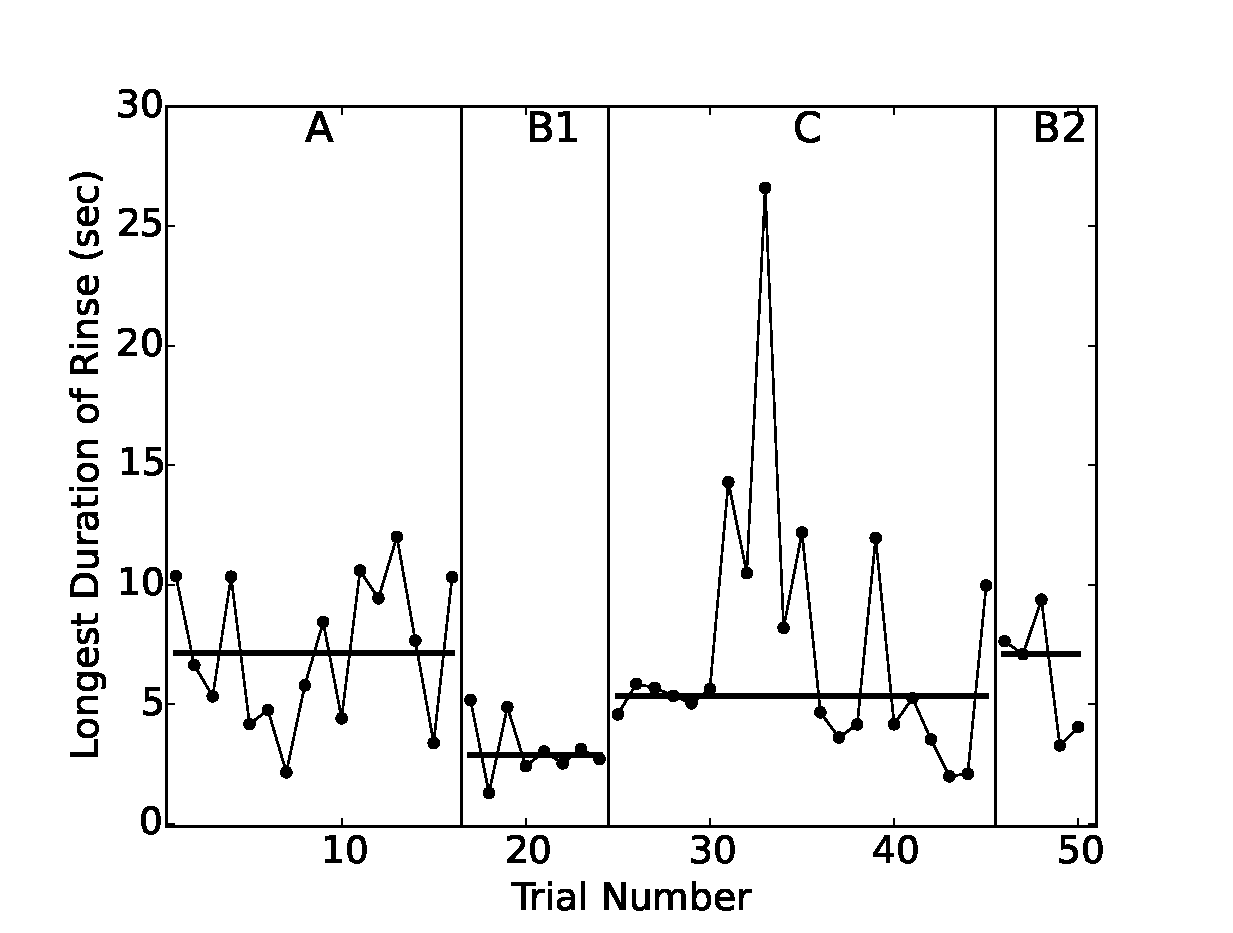
\includegraphics[width=0.6\textwidth]{./img/data_analysis/8LongestDurationofRinsesec.eps}
%DIFDELCMD < 	%%%
%DIFDELCMD < \caption{%
{%DIFAUXCMD
\DIFdelFL{Longest Duration of Rinse Step}}
	%DIFAUXCMD
%DIFDELCMD < \label{fig:8LongestDurationofRinsesec}
%DIFDELCMD < \end{figure}
%DIFDELCMD < 

%DIFDELCMD < %%%
\subsection{\DIFdel{Qualitative Analysis and Results - Further}}
%DIFAUXCMD
\addtocounter{subsection}{-1}%DIFAUXCMD
\DIFdel{After confirming our initial qualitative analysis results through quantitative measures on the child's improvements, we continue our qualitative analysis to answer what factors contributed to these improvements through parent researcher interview discussions and researcher self reflection.
}%DIFDELCMD < 

%DIFDELCMD < %%%
\DIFdelend \subsubsection{Causes of Child's Non-Compliances}
Between trials, the researcher (also taking the role of the robot operator) had frequent interview discussions with the mother (referred to as ``the parent'' in previous sections), and occasionally with the father, regarding reasons why the child had problems following the robot.

One major problem pointed out by both of the parents as well as the operator was the delay between each robot prompts.  This problem was particularly significant for our participant, who knew most of the steps of hand-washing, and only needed robot prompts to get started, to terminate the soap step, to rinse more, and to dry more.  Because of his familiarity with the hand-washing steps, he finished each step very quickly and was eager to move to the next step.  Thus a slight delay from the robot would result in the child not waiting for the robot prompts and proceeding on his own.  The mother first pointed this out in \DIFdelbegin \DIFdel{the first Phase B}\DIFdelend \DIFaddbegin \DIFadd{Phase B1}\DIFaddend , and the operator echoed her opinion, reflecting that it is hard to make the robot keep up with the child due to his pace and the robot delay.  The father also confirmed the opinion in \DIFdelbegin \DIFdel{the second Phase B }\DIFdelend \DIFaddbegin \DIFadd{Phase B2 }\DIFaddend that there should be less pause between prompts, especially for the rinse more prompts, as to prevent the child from moving onto the next step on his own.  Note that the father's opinion was based on the robot behavior after its improvements made to shorten its delays.

In addition, the parents proposed that unfamiliarity was a major cause of the child not following the robot prompts.  One possible cause for the child's noncompliance was his unfamiliarity with the robot and the washroom environment.  Both parents suggested that the child would be more relaxed and likely not rush each step if he was in a familiar environment, such as at home.  Furthermore, compliance would be greatly improved if the child and the robot built a relationship over time, the mother suggested, and if the robot was always there telling the child what to do, said the father.  To \DIFdelbegin \DIFdel{expend }\DIFdelend \DIFaddbegin \DIFadd{expand }\DIFaddend on his point, the father explained that the robot needed not to be an authoritative figure like his parents, but just needed to be a figure that the child is familiar in following instructions from, as exemplified by the child's tendency in following his younger brother's instructions.  The father further claimed that it was familiarity and routine, not trust.  The researcher noted that the environmental conditions between the parent trials and the robot trials were similar.  Thus, although being familiar with the environment would possibly improve compliance, the factor that contributed to the difference of child's compliance to the robot and to the parent can only be attributed to his unfamiliarity with the robot, not the environment.

Another possible cause for the child's noncompliance was fatigue due to repetitive consecutive hand-washing trials.  As pointed out by the father, during the robot trials, the child has been asked to wash his hands ten times in a roll with only five minutes of break between each time.  In addition, the robot prompted the rinse step for more than fifteen seconds each time, both of these may make the child unwilling to follow.  The father suggested to conduct each trial two to three hours apart, and prompt rinsing for only ten to fifteen seconds each time.  After further investigation, the researcher noted that the child's fatigue behavior was not specific to the robot, but also present during Phase A when the parent alone prompted the child.  The behavior manifested in the form of the child not willing to rinse more, but the exhibition of it was more subtle in the parent prompting case -- the child would comply to the parent's rinse more prompts, but he would only put his hands into the water for one second and quickly withdrew them and turned to look at the parent for approval to proceed to the next step, where as the child would openly refuse to rinse more in the robot's case.

Another possible cause for noncompliance was the child being confused of what was prompted or what was expected of him by the prompt.  However, there were evidences that the child understood most of the robot verbal prompts, if not all, because he was able to follow them at some point or another.  Thus, for the steps that the child did not follow, one can argue that it must have been due to a cause other than being generally confused of what was prompted.  The mother also confirmed that she thought the child was not confused by the robot prompts.  There were occasions when the child was confused, and they were when the parent pointed to the towel for the child to dry more after the child decided to leave the washroom.  The child would often mistook the parent's pointing gesture for rinse more, and started rinsing again instead of drying.  No such behavior occurred for robot prompts.


\subsubsection{Causes of Improvements of Child's Compliance}
There were three major factors identified by the researcher in potentially causing the improvements observed in the child's compliance to robot prompts: the first one was the improvements made to reduce robot prompt delays; the second was the child's gradual adjusting to the robot and to the routine of following its prompts; and the third was the effect of the trials in Phase C when the parent trained the child to follow the robot prompts.  Of course, there might be other important factors that happened during the time the child spent outside of the lab that were unaccounted for.

In regards to these three factors, the robot prompt delay improvement was seen as the least significant, since even after the improvement, we still could not achieve the responsiveness that the parent had during prompting.  The father also expressed he was not satisfied with the improved robot's responsiveness.   In addition, the effect on child's compliance by increasing the robot's responsiveness to the level of the parent was still unknown.

As to the other two factors, both involved the child learning to be guided by the robot, one from natural familiarization by himself and the other due to artificial training from the parent.  One may argue that, since the improvements mostly occurred after the second half of Phase C, it may suggest that the effect of artificial training from the parent was more dominant, since if it was the other way, then the child would have shown improvements earlier (e.g. after \DIFdelbegin \DIFdel{the first Phase B }\DIFdelend \DIFaddbegin \DIFadd{Phase B1 }\DIFaddend or during first half of Phase C).  However, this claim still lacks concrete evidence, and this question should be answered more rigorously by introducing a longer \DIFdelbegin \DIFdel{first Phase B }\DIFdelend \DIFaddbegin \DIFadd{Phase B1 }\DIFaddend that is comparable to Phase C (in our study, we had one week for \DIFdelbegin \DIFdel{first Phase B}\DIFdelend \DIFaddbegin \DIFadd{Phase B1}\DIFaddend , but two weeks for Phase C) so that the learning effects of the two phases can be compared.


\subsubsection{Post-Intervention Survey for Parent}
The post-intervention survey results are presented in Table \ref{tab:PostInterventionSurveyData}.  \DIFaddbegin \DIFadd{For each statement, the parent had a choice of strongly agree, Agree, Neither agree nor disagree, disagree, and strongly disagree.  }\DIFaddend We see that the parent was happy with all aspects of the robot as a prompting agent, but did not see it to be as good as herself yet in delivering effective prompting.

In addition, the suggestions the parent made regarding the robot and the experiment are reported:  The robot can improve its pointing better so that the child sees exactly which object he needs to interact with.  This can be done by having more fingers on the robot's hands, or by attaching a light source (e.g. laser pointer or mini-projector) that the robot can use to highlight physical objects at the sink.  The robot would be more visible if it is bigger or placed at eye level of the child.  It would be ideal if the robot is mobile, and can prompt other activities of daily living besides hand-washing.  Lastly, attaching permanent cameras in the washroom is not okay, since the child is not the only one using the washroom.  Thus, having a mobile robot that follows the child would be a better solution.





\DIFdelbegin %DIFDELCMD < \begin{table}[H]
%DIFDELCMD < 	\centering
%DIFDELCMD < 	\begin{tabular}{ | p{12cm} | l | }
%DIFDELCMD < 		\hline
%DIFDELCMD < 		%%%
\textbf{\DIFdelFL{Survey Question}}	%DIFAUXCMD
%DIFDELCMD < &	%%%
\textbf{\DIFdelFL{Parent's Answer}}	%DIFAUXCMD
%DIFDELCMD < \\	\hline	\hline		
%DIFDELCMD < 		%%%
\DIFdelFL{Hand-washing steps break down was appropriate	}%DIFDELCMD < &	%%%
\DIFdelFL{Strongly Agree	}%DIFDELCMD < \\	\hline
%DIFDELCMD < 		%%%
\DIFdelFL{My child understood the verbal prompts	}%DIFDELCMD < &	%%%
\DIFdelFL{Agree	}%DIFDELCMD < \\	\hline
%DIFDELCMD < 		%%%
\DIFdelFL{Robot's verbal prompts were appropriate	}%DIFDELCMD < &	%%%
\DIFdelFL{Strongly Agree	}%DIFDELCMD < \\	\hline
%DIFDELCMD < 		%%%
\DIFdelFL{The prompt wordings were similar to mine	}%DIFDELCMD < &	%%%
\DIFdelFL{Strongly Agree	}%DIFDELCMD < \\	\hline
%DIFDELCMD < 		%%%
\DIFdelFL{The prompt voice and tone were appropriate	}%DIFDELCMD < &	%%%
\DIFdelFL{Strongly Agree	}%DIFDELCMD < \\	\hline
%DIFDELCMD < 		%%%
\DIFdelFL{The prompt wordings were easy to understand	}%DIFDELCMD < &	%%%
\DIFdelFL{Strongly Agree }%DIFDELCMD < \\	\hline
%DIFDELCMD < 		%%%
\DIFdelFL{My child understood the gesture prompts	}%DIFDELCMD < &	%%%
\DIFdelFL{Strongly Agree	}%DIFDELCMD < \\	\hline
%DIFDELCMD < 		%%%
\DIFdelFL{The gesture prompts were appropriate	}%DIFDELCMD < &	%%%
\DIFdelFL{Strongly Agree	}%DIFDELCMD < \\	\hline
%DIFDELCMD < 		%%%
\DIFdelFL{The gesture prompts were easy to understand	}%DIFDELCMD < &	%%%
\DIFdelFL{Agree	}%DIFDELCMD < \\	\hline
%DIFDELCMD < 		%%%
\DIFdelFL{The physical appearance of robot is aesthetically pleasing	}%DIFDELCMD < &	%%%
\DIFdelFL{Agree	}%DIFDELCMD < \\	\hline
%DIFDELCMD < 		%%%
\DIFdelFL{The attention grabber gestures were appropriate	}%DIFDELCMD < &	%%%
\DIFdelFL{Strongly Agree	}%DIFDELCMD < \\	\hline
%DIFDELCMD < 		%%%
\DIFdelFL{The verbal rewards were appropriate	}%DIFDELCMD < &	%%%
\DIFdelFL{Strongly Agree	}%DIFDELCMD < \\	\hline
%DIFDELCMD < 		%%%
\DIFdelFL{The reward gestures were appropriate	}%DIFDELCMD < &	%%%
\DIFdelFL{Strongly Agree	}%DIFDELCMD < \\	\hline
%DIFDELCMD < 		%%%
\DIFdelFL{The robot was effective in assisting my child through hand-washing	}%DIFDELCMD < &	%%%
\DIFdelFL{Strongly Agree	}%DIFDELCMD < \\	\hline
%DIFDELCMD < 		%%%
\DIFdelFL{The robot motivated my child to wash hands	}%DIFDELCMD < &	%%%
\DIFdelFL{Strongly Agree	}%DIFDELCMD < \\	\hline
%DIFDELCMD < 		%%%
\DIFdelFL{The robot was fun for my child to use	}%DIFDELCMD < &	%%%
\DIFdelFL{Strongly Agree	}%DIFDELCMD < \\	\hline
%DIFDELCMD < 		%%%
\DIFdelFL{My child was confused by the robot	}%DIFDELCMD < &	%%%
\DIFdelFL{Disagree	}%DIFDELCMD < \\	\hline
%DIFDELCMD < 		%%%
\DIFdelFL{I like the idea of a robot prompting my child	}%DIFDELCMD < &	%%%
\DIFdelFL{Strongly Agree	}%DIFDELCMD < \\	\hline
%DIFDELCMD < 		%%%
\DIFdelFL{The robot is able to provide guidance as well as I can or better	}%DIFDELCMD < &	%%%
\DIFdelFL{Neither Agree or Disagree	}%DIFDELCMD < \\	\hline
%DIFDELCMD < 		%%%
\DIFdelFL{I would want to own a robot like this one	}%DIFDELCMD < &	%%%
\DIFdelFL{Strongly Agree	}%DIFDELCMD < \\	\hline
%DIFDELCMD < 	\end{tabular}
%DIFDELCMD < 	%%%
%DIFDELCMD < \caption{%
{%DIFAUXCMD
\DIFdelFL{The Post-Intervention Survey Data}}
	%DIFAUXCMD
%DIFDELCMD < \label{tab:PostInterventionSurveyData}
%DIFDELCMD < \end{table}
%DIFDELCMD < 

%DIFDELCMD < %%%
\DIFdelend \section{Discussion}
A Wizard of Oz study has been conducted following the A-B-C-B case study design on a single participant.  In Phase A, the parent alone prompted the child through hand-washing steps.  In \DIFdelbegin \DIFdel{first Phase B}\DIFdelend \DIFaddbegin \DIFadd{Phase B1}\DIFaddend , the robot alone prompted the child.  In Phase C, the parent and the robot jointly prompted.  In \DIFdelbegin \DIFdel{second Phase B}\DIFdelend \DIFaddbegin \DIFadd{Phase B2}\DIFaddend , the robot alone prompted the child again.  Parent researcher interview was conducted during breaks between trials.  Both qualitative and quantitative analyses were conducted on the study data, and we observed promising results.


\subsection{Summary of Results}
We saw that, although the child did not listen to the robot as much as \DIFdelbegin \DIFdel{it }\DIFdelend \DIFaddbegin \DIFadd{he }\DIFaddend did to the parent when the robot was first introduced, through a parent robot joint training phase, the child showed drastic improvement in robot prompt compliance, approaching the compliance level achieved by the parent prompts.  Although our participant did not appear to need help in how to execute each hand-washing steps, he did need prompting to get the hand-washing started and stay on task, and supervision on scrubbing, rinsing and drying longer and not getting too much soap.  Our analyses showed that through training, the robot was \DIFdelbegin \DIFdel{able to achieve }\DIFdelend \DIFaddbegin \DIFadd{successful in }\DIFaddend getting the child to meet most of these goals.  Specifically, the \DIFaddbegin \DIFadd{qualitative analyses showed that the }\DIFaddend child waited for the robot to prompt first before starting the hand-washing activity.  Also, the child followed the robot's rinse prompts and rinsed longer as a result.  However, the robot was only somewhat successful in getting the child to move on from the soap step, and was unsuccessful in getting the child to scrub hands or to dry hands longer.  The parent, on the other hand, had no problems in getting the child to scrub hands, but she did have some difficulties in getting the child to dry longer and had definite difficulties in getting the child to move on from the soap step.

\DIFdelbegin \DIFdel{The parent }\DIFdelend %DIF > \subsection{Quantitative Analysis and Results - Further}
%DIF > After qualitative analysis, we saw that the child improved in robot prompts compliance through the training Phase C and retained those improvements in Phase B2.  Specifically, the greatest improvements were that the child was waiting for the turn on water robot prompt before executing, the child complied more to robot rinse prompts, and not terminating by himself as much during rinsing.  
%DIF > 
\DIFaddbegin \DIFadd{To further validate these qualitative findings further and quantify the improvements, we here created and analyzed the following measures:
}\begin{itemize}
	\item \textbf{\DIFadd{Not Waiting For Turn On Water Prompt Rate}}\DIFadd{: the percentage of trials in a phase that the child does not wait for the turn on water prompt from the robot (i.e. starts executing that step by himself).
	}\item \textbf{\DIFadd{Rinse Step Complied Prompt Rate}}\DIFadd{: the percentage of prompts for the rinse steps in a trial that the child followed by showing an effort of attempt.
	}\item \textbf{\DIFadd{Longest Duration of Rinse Step}}\DIFadd{: the longest duration in seconds in a trial that the child rinses hands continuously without terminating.
}\end{itemize}
\subsubsection{\DIFadd{Not Waiting For Turn On Water Prompt Rate}}
\DIFadd{The Not Waiting For Turn On Water Prompt Rate for Phase A is 6 out of 16 trials = 37.5\%, for Phase B1 is 5 out of 8 trials = 62.5\%, for Phase C is 5 out of 21 trials = 23.8\%, for Phase B2 is 2 out of 5 trials = 40\%.  We see an improvement of the child in waiting for the robot's turn on water prompt in training Phase C, and a retained improvement (although with a slight slide back) in Phase B2.
}

\subsubsection{\DIFadd{Rinse Step Complied Prompt Rate}}
\DIFadd{The Rinse Step Complied Prompt Rate is plotted in Figure \ref{fig:5CompliedPromptRate-RinseStep}, and has a median for Phase A of 100\%, for Phase B1 of 33\%, for Phase C of 100\%, for Phase B2 of 75\%.  Despite variance in data, we see that the improvement in rinse step robot prompt compliance is retained in Phase B2.
}\begin{figure} [H]
	\centering
	\includegraphics[width=0.6\textwidth]{./img/data_analysis/5CompliedPromptRate-RinseStep.eps}
	\caption{\DIFaddFL{Rinse Step Complied Prompt Rate}}
	\label{fig:5CompliedPromptRate-RinseStep}
\end{figure}

\subsubsection{\DIFadd{Longest Duration of Rinse Step}}
\DIFadd{The Longest Duration of Rinse Step is plotted in Figure \ref{fig:8LongestDurationofRinsesec}, and has a median for Phase A of 7.15s, for Phase B1 of 2.87s, for Phase C of 5.36s, and for Phase B2 of 7.09s.  We see that the rinse step duration in Phase B1 was especially short, and was improved in Phase B2.
}\begin{figure} [H]
	\centering
	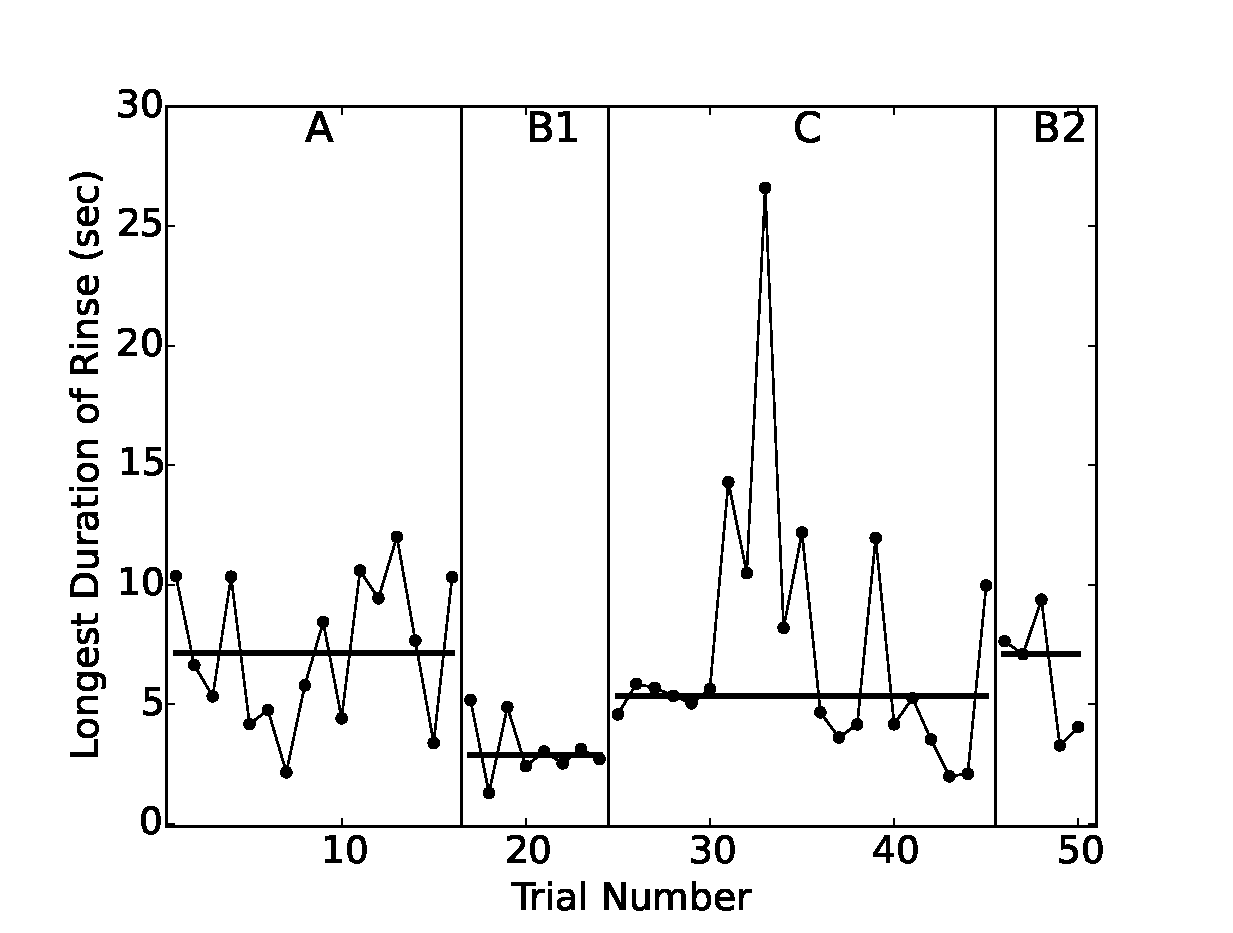
\includegraphics[width=0.6\textwidth]{./img/data_analysis/8LongestDurationofRinsesec.eps}
	\caption{\DIFaddFL{Longest Duration of Rinse Step}}
	\label{fig:8LongestDurationofRinsesec}
\end{figure}
\DIFadd{In whole, these confirm the finding that the child's improvements in responding to robot in training Phase C are retained in Phase B2.
}

\DIFadd{The way the robot prompted was verified to be very similar to how the parent prompted.  The parent }\DIFaddend was not instructed in the specifics of how to prompt -- she prompted in the most natural way she and the child were used to, and yet there were a lot of similarities between the parent and the robot's prompting patterns.  First, they shared similar breakdown of the hand-washing steps, although the parent referred to the scrub step as lather.  In addition, the both the parent and the robot prompted by giving verbal instructions along with some form of gesture prompts.  The differences were that the parent used more pointing and less motion demonstration, and that the motion demonstrations from the parent were much faster moving than the robot's (especially for the scrub step).  The child paid much more attention to the parent's faster moving motion demonstrations than the robot's, and is one area of future improvements.  Other design recommendations for the robot included faster response times to child's behaviors, issuing a fast attention grabber accompanied with increased severity in tone of voice when the child is non-compliant, and rewarding the child for major steps only (e.g. the end of rinsing and drying steps).  Other design recommendations raised by the parent and the researcher mainly involved engaging the child better, including more dynamic motions for gestures, playing cartoon noises for rewards or attention grabbers, having a bigger robot so it is more visually engaging, etc.

In terms of modes of interactions needed between the child and the robot for successfully helping the child to wash hands, the delivering of verbal and gestural prompts with at least two levels of severity (more severe sounding and looking prompts delivered when the child is non-compliant) were definitely needed.  However, the detection of the visual focus of attention of the child showed little value.  The child's visual attention was hardly an indicator of engagement at all.  On the other hand, we found that understanding verbal feedbacks from the child may be useful as the child verbally repeated instructions when he was processing them, and murmured back in protest when he did not wish to follow certain prompts.  Utilizing these speeches as indication of the child's engagement may be useful in adjusting robot prompts to better suit the child's needs.  Also, we observed that the child did not like prolonged rinsing, and what the parent did was to stop prompting the rinse step and to move on to the next step when the child showed non-compliant behavior through rinsing for only a second and quickly removing his hands from the water.  The robot did not move on and repeated the rinse prompts in hope the child would follow, and as a result, the child often moved on by himself without waiting for the robot.  In future studies, the robot should also implement a way to work with the child to rinse as much as possible but learn to move on when the child shows signs of non-compliance.


\subsection{Internal and External Validity}
In this section, our results are critically reviewed based on data collection, analysis methods, and result interpretations.  Possible sources of errors, competing interpretations, limitations of results, and their generalizability are discussed.

\subsubsection{Quantitative Analysis Method}
The choice of measures used in the quantitative analyses were based on our study objectives and chosen in light of the qualitative analysis results, in an attempt to answer the question ``Is the robot NAO able to guide our participant, a child with ASD, through hand-washing?".  ``Number of Steps Completed'' only reflected the variety of steps completed, but did not measure the quality of the completed steps.  Thus it could only partially confirm how well the robot guided the child.  ``Longest Duration of Rinse Step'' was our attempt to measure the quality of the rinse step completed.  The rinse step was chosen due to the drastic improvement the child exhibited on this particular step, and the duration of the longest rinse was the most obvious way to measure the quality of the rinse step completion.  One thing to note is, the parent, during the training phase, focused most of her prompts on getting the child to follow the rinse prompts from the robot, but very little prompts were focused on the dry hands prompts.  Consequently, we did not experience as much improvement on the duration of dry hands step.  To link the child's success in completing all steps and with good quality to the prompting agents, the ``Compliance Rate'' and the ``\DIFdelbegin \DIFdel{Not Affected By }\DIFdelend \DIFaddbegin \DIFadd{Ignored }\DIFaddend Prompt Rate'' were measured, for all steps (and Compliance Rate for the rinse step particularly as well).  We see that the robot had much more influence on the child in \DIFdelbegin \DIFdel{second Phase B}\DIFdelend \DIFaddbegin \DIFadd{Phase B2}\DIFaddend , but not in \DIFdelbegin \DIFdel{first Phase B}\DIFdelend \DIFaddbegin \DIFadd{Phase B1}\DIFaddend , and this resulted in an increased duration of rinse in \DIFdelbegin \DIFdel{second Phase B}\DIFdelend \DIFaddbegin \DIFadd{Phase B2}\DIFaddend .  Thus, we concluded that the robot was successful in improving the quality of hand-washing of our child with ASD.  But since the child already knew all the steps and was able to complete all steps in \DIFdelbegin \DIFdel{first Phase B }\DIFdelend \DIFaddbegin \DIFadd{Phase B1 }\DIFaddend with minimal influence from the robot, no conclusions can be made regarding whether the robot could successfully teach our child with ASD a new hand-washing step.

Medians were used as a fair and reliable way of comparing the measures across phases.  The choice of median, as opposed to mean, was out of the consideration for robustness against outliers.  This may be a good choice if the data had relatively low variance and few outliers.  However, our data contained high variance, and the definition of outliers became blurred.  Take ``Rinse Step Compliance Rate'' (seen in Figure \ref{fig:5ComplianceRate-RinseStep}) for example.  The rate in Phase C has a median of 100\%, but there are a third of data points in this phase falling below 80\%.  Thus, one obvious question is, why have we not used some form of description of variance alongside our description of data centers (i.e. median) in our across phase comparisons?  The reasoning was that the low sample size for some phases (e.g. \DIFdelbegin \DIFdel{second Phase B }\DIFdelend \DIFaddbegin \DIFadd{Phase B2 }\DIFaddend only has 5 data points) made any analysis based on variance not statistical significant.  This is a limitation of our study results, but given the pilot nature of our study, it is acceptable since it yielded promising results confirming the direction of future studies.

Another limitation exists in our lack of control on video data annotation errors.  For a more rigorous future study, more than one person should carry out the data annotations, and the degree of annotator subjectiveness can then be characterized by an inter-rater agreement measure such as the Cohen's Kappa \cite{volkmar2005handbook}.

\subsubsection{Qualitative Analysis Method}
The qualitative analyses of our study employed several strategies to ensure internal validity.  These strategies being reviewed include triangulation, member checks, adequate engagement in data collection, reseracher's position or reflexivity, peer review / examination, audit trial, rich thick description, an maximum variation \cite{merriam2014qualitative}.  Firstly, we employed triangulation by using multiple investigators and sources of data to confirm findings.  The observations of the child's behaviors and possible robot design recommendations were made by the researcher through making field notes of the trials video data, by the parents through the parent researcher interview discussions and the post intervention survey.  Secondly, during the parent researcher interviews, due to the interactive nature of the interview format, the member check technique was inherent.  The researcher was able to check his understanding of the emerging findings with the parent to ensure minimal misinterpretation was made.  \DIFdelbegin \DIFdel{Thirdly, we did not employ the adequate engagement in data collection technique satisfactorily.  Phase A and first Phase B were carried out long enough to see saturation of findings, but due to limitation of time, training Phase C and second Phase B were not carried long enough to such saturation.  Especially, the training Phase C could have been longer to see possibly even further improvement of the child, and the second phase C could have been longer (at least to match the length of the first Phase B) to eliminate any doubts that the improvements observed in training phase were successfully retained.  }\DIFdelend In regards to researcher's position or reflexivity, the researcher \DIFdelbegin \DIFdel{must confess that he has little training in research with }\DIFdelend \DIFaddbegin \DIFadd{was trained mainly in the engineering discipline and had limited experience and expertise in teaching }\DIFaddend children with ASD\DIFdelbegin \DIFdel{or in any general human behaviors research}\DIFdelend .  Such lack of experience may prove invalid any opinion the researcher had on the child's behaviors and on the reasons behind them.  However, the researcher relied heavily on the parents' interpretation of the child's behaviors, preferences, and possible reasons behind his behaviors instead.  \DIFdelbegin \DIFdel{And the }\DIFdelend \DIFaddbegin \DIFadd{The }\DIFaddend parents, being both experienced with the child's needs in particular and trained with knowledges of children with ASD in general, were very adequate observers used by our study.  In addition, audit trail and rich, thick descriptions were used to compensate the researcher's interpretation errors.  By providing a detailed account of the backgrounds, methods, procedures, and decisions made when conducting the study, the value of the study results can be critically assessed based on contexts by other researchers themselves when reading this thesis.  Lastly, during the training phase, the parent involvements were purposefully varied through the phase.  This maximum variation technique allowed greater diversity in sample selection, enabling a greater range of findings and possible applications of the findings.

\DIFaddbegin \DIFadd{In whole, the study was mostly carried out and analyzed rigorously.  However, the study was limited in that we did not collect data to saturation.  Phase A and Phase B1 were carried out long enough to see saturation of findings, but due to limitation of time, training Phase C and Phase B2 were not carried long enough to such saturation.  Especially, the training Phase C could have been longer to see possibly even further improvement of the child, and the second phase C could have been longer (at least to match the length of Phase B1) to eliminate any doubts that the improvements observed in training phase were successfully retained.
}

\DIFaddend \subsubsection{Confounding Variables}
Due to the study protocol and the research design, there were several uncontrolled variables that may have confounded our results, threatening the internal validity of our results.

One confounding variable was the change of robot control scheme in the middle of \DIFdelbegin \DIFdel{the first Phase B}\DIFdelend \DIFaddbegin \DIFadd{Phase B1}\DIFaddend .  The reason for change was because our participant required a much more reactive robot who can switch the current step being prompted on the fly.  As stated in the study protocol, if any essential improvements of the robot (or the study procedures) were made apparent through the ongoing analysis, we would implement the change.  After the control scheme switch, both the parent and the robot operator (the researcher) felt the robot was more responsive to the child.  However, the parent did report that the robot was still too slow for the child, and sometimes the pause between robot actions were still too long.  This confounding variable had a sudden change, and we expected to also see sudden changes in our dependent measures shortly following the effect.  However, this was not observed, and may be due to the effect size of this confounding variable was too low compared to the level of noises in our measures.  Another possibility is that some inherent nature of the child made him remaining to behave a certain way despite changes in stimulus.  Either way, this confounding variable does not threaten our results that the robot was eventually able to help the child through hand-washings.  However, it may threaten the hypothesis that it was the training phase instead of the robot control scheme change that caused the improvements in the child's behaviors towards the robot.

Another confounding variable was the fact that the current study (Wizard of Oz) involved a human operator (the researcher) remotely controlling the robot.  The researcher had no experience guiding the participant through hand-washing prior to the study, and thus it was a learning process for the researcher through out the study as well.  This meant that the researcher changed the order of steps the robot prompts were delivered to best fit the child's preference (e.g. the child preferred to put on soap before turning on water).  Also, the researcher chose prompts that were more effective (e.g. the attention grabber was not effective and so was not used in the end, and the child did not distinguish between scrub hands and rinse hands, so scrub hand prompts were not used in the end).  These changes were gradual, but may play a confounding effect on our measures, threatening the hypothesis that the training phase was the sole cause of the child's improvements.  In addition, in the future when we will be automating the robot behaviors, tuning the robot prompts and order of steps to each child's preference will be an inevitable part of the automation process.

The researcher was not the only one learning, the child in fact was learning and familiarizing with the robot prompts, the experiment environment, and the hand-washing activity in this environment.  Children with ASD are very \DIFdelbegin \DIFdel{peculiar }\DIFdelend \DIFaddbegin \DIFadd{particular }\DIFaddend about keeping routines in a familiar environment.  Thus, introducing the robot, which the child did not have any prior experience to playing with or following orders from, in a foreign washroom with unfamiliar washroom setups, created a barrier for the child to put on his best responses to the robot prompts.  Since the parent alone prompting phase (Phase A) also had the unfamiliarity of environment confounding effect, this confounding variable does not threaten the conclusion that the robot did not perform as well as the parent as a prompting agent.  But the reason for this inequality in performance can be explained by the robot being inferior to the parent as a prompting agent by nature, or can be explained by the fact that the child was much used to following orders from the parent than the robot.  In addition, the child's unfamiliarity and learning to get used to being prompted by and following the robot, was also the alternative explanation of his improvements, competing with the training phase explanation.  Lastly, the child was already skilled in most of the hand-washing steps, thus little learning or improvements over the completion of steps were observed.  Instead, the only rooms for improvements were on the quality of step completion for scrubbing, rinsing, and drying.  Thus, our result that the robot was able to improve the child's rinse duration may have been confounded by the fact that the child could have improved in this regard with or without the robot's presence.  However, our results that the child did not recede to shorter rinse durations in \DIFdelbegin \DIFdel{second Phase B }\DIFdelend \DIFaddbegin \DIFadd{Phase B2 }\DIFaddend (when being prompted alone by the robot) remained unchallenged by this confounding variable.

The last confounding variable is fatigue.  This variable was identified by the parents as well as the researcher when observing the child's behaviors.  Because of the number of repetitions of hand-washing conducted as well as the long durations of rinse in each hand-washing, the child quickly became fatigued and unwilling to comply to rinsing and sought to finish the remaining of the steps as quickly as possible.  This confounding variable introduced noises to our measures, burying important patterns that may have otherwise been observed.  In future studies, long duration of rinse (around 12 seconds) can still be required, but the repetitions must be avoided by having less than five hand-washings each day and spread them sparsely through the day.  Logistically, this would mean conducting the research in a school or home wash-room, where the child carries everyday activities, rather in a laboratory.

\subsubsection{Generalizability}
Our study only had one participant.  This means our results \DIFdelbegin \DIFdel{maybe only }\DIFdelend \DIFaddbegin \DIFadd{may only be }\DIFaddend applicable to this particular child, but not generalizable to the \DIFdelbegin \DIFdel{whole children with }\DIFdelend ASD population.  The next study in the future should increase the number of participants \DIFdelbegin \DIFdel{(maybe around ten subjects) }\DIFdelend while validating the major results of the current study.  The single subject research design should be used for this future study, since due to the diverseness of the children with ASD population, measures may have different levels across subjects.  Thus, we should generalize the effectiveness of an intervention by comparing the amount of change of measure levels for each child when having the intervention compared against that same child not having the intervention.  Also, the secondary aim of this future study is to find out the participant demographics of a subpopulation of children with ASD that our intervention works consistently well on.  Only after this future study validating our major results and after we choose a subpopulation to focus on, should we attempt a larger scale \DIFdelbegin \DIFdel{(maybe around thirty subjects) }\DIFdelend randomized control trial, in which we divide the participants into control and intervention groups, and generalization of intervention effectiveness is made by directly comparing the measure levels between groups.  The focus of this randomized control would be to show clinical effectiveness of our intervention on the focused subpopulation.

The robot showed promising results in supervising our child with ASD, who already knew the basics of the hand-washing steps, but only needed guidance on the initiation and termination of steps.  It is still unknown how our robot would perform in teaching children with ASD the motions of hand-washing steps.  The parents and the researcher were not satisfied with the robot's dexterity, and worried that this lack of complexity of the robot's hands would not be adequate in teaching the child complex hand-washing motions such as scrubbing or drying.  Future study should explore this aspect further with children with ASD who have not learned the specifics of hand-washing step motions yet.

One more limitation existed in our experiment protocol, specifically in regulating how the parent prompts in Phase C.  During Phase C, where the parent prompts the child alongside the robot, we gave the parent freedoms to decide how best to prompt.  Firstly, the parent could choose between verbal prompting in competition with the robot prompts, verbal prompting complementary to robot prompts, and physical prompting complementary to robot prompts [sec ref].  The parent decided to focus on the latter two, and alternated between the two as she saw fit.  Secondly, the parent could decide when to prompt relative to robot prompts.  In general, the parent prompted immediately after the robot.  However, there are cases where the parent prompts simultaneously with the robot, or even before the robot.  Our result that Phase C acted as a training phase that resulted in effectiveness improvement of robot prompts still holds.  What it does affect, though, is that we do not know which variable regarding how the parent prompts in Phase C was most beneficial in improving robot prompt effectiveness.  Thus, in future experiments, controlling how the parent prompts in the training phase is needed to better understand how to consistently improve robot prompt effectiveness.

In addition, the intensity of our training, although very repetitive in each visit, was very sparse in a weekly schedule.  There was only one visit each week, and the training only lasted two weeks.  It was our hypothesis that, if we implemented a more intensive training, maybe three times a day, seven days a week, and maybe for a month of duration, we would achieve complete independence of parent in using the robot to guide the child through hand-washing.  Longitudinally focused intensive training may be one possible direction of future study.

Our study was conducted in the washroom of the HomeLab, in the Toronto Rehab \DIFdelbegin \DIFdel{Hospital}\DIFdelend \DIFaddbegin \DIFadd{Institute}\DIFaddend .  This experimental setting is a controlled environment, where camera can be installed anywhere we desired to best capture and analyze the study.  The use of camera is essential for the robot (or the operator) in tracking and understanding the child's progress during the hand-washing.  Eventually, when the robot is automated, the operator will be replaced by AI and computer vision algorithms, which will still rely on the cameras as sensor input.  The parents raised the concern that installing cameras on the washroom wall, in the way we did in our study, was not possible at the home settings.  They voiced that they are willing to make the compromise of having their child with ASD being under the camera in the washroom if this will help him independently execute ADLs, but they are not willing to have any other member of the family under the camera.  The solution to this would be to have a mobile robot that follows the child with ASD, and the camera will be attached onto the robot instead of fixed in the washroom.  The feasibility of such setup was not tested in our study, and should be employed in future studies, in the home or in the laboratory settings.

In whole, we learned from our study that the robot was a promising prompting agent in supervising the child with ASD through hand-washing.  It is not hard to hypothesize that such success can be replicated in other ADLs such as tooth-brushing, putting on clothes, or cooking.  Future studies may investigate the robot's effectiveness in prompting these other ADLs.  However, one immediate question follows: is robot the best prompting agent available for helping children with ASD through ADLs?  The successes we had with the robot prompts were mainly due to its ability to deliver verbal and gesture prompts.  However, a multimedia system with a LCD monitor could deliver similar prompts, by having a virtual avatar displayed on screen carrying out the robot prompts the same way.  The key difference lies that such system lacks embodiment in the physical world.  It may be worthwhile to compare the impact of this embodiment in effectiveness of the prompting agent in future studies.  If similar effectiveness is observed, the virtual avatar prompting agent may be the cost effectiveness solution that may be commercially available to families with children with ASD immediately.

%\subsection{Research Significance}
%significance:	
%	- what gaps have we achieved to fill in our study results?  should we continue this line of research? why or why not?  in what direction should we best continue?
%	- also discuss how are the results related to literature and what research gap it fills, i.e. significance of results (might need generalization analysis), talk about scientific contribution of our study and results
%	- The value this thesis is not only the conclusions it might make, but also the methodology.  Basically, it's the first study of its kind, and employed new analysis framework instead of adopting existing methodology.  Took me a while to do the video annotation framework.  Need to emphasize this contribution's significance.



\chapter{Visual Focus of Attention Estimation}
From the WoZ pilot study, we \DIFdelbegin \DIFdel{have }\DIFdelend learned that our participant did not look at the robot as often as expected during prompting.  This meant either that the robot and its actions were not visually stimulating enough to motivate the participant to focus his attention upon or that he was not interested in observing the motions demonstrated possibly because he already knows them.  Although no relationships between the Visual Focus of Attention (VFOA\DIFaddbegin \DIFadd{) }\DIFaddend on robot and \DIFdelbegin \DIFdel{Compliance }\DIFdelend \DIFaddbegin \DIFadd{Complied Prompt }\DIFaddend Rate were observed for our participant, literatures suggest that keeping the child with ASD visually engaged during action modeling when teaching a new skill is essential [\ref{Sec:AT4ASDDiscussion}].  Thus, for future studies with participants that are not familiar with the hand-washing motions, it is still helpful to be able to track the VFOA of the child with ASD during the hand-washing activity, so that the robot actions may adjust automatically to better engage the child's visual attention.

To track the VFOA of the child, we used the Microsoft Kinect to collect RGB and depth images of the child's head.  Gaze directions can be tracked more accurately when head is viewed near frontal, and since we cared more about the child's attention to prompting agents than to sink objects, we setup the Kinect near the robot, and have sink objects further from the Kinect (i.e. soap and towel) be spread apart from each other to be easily distinguished.

The problem of estimating the object under child's attentional focus is broken into three parts: head pose estimation, eye pose estimation, and object identification.


%Overall objective
%	- to implement a real time gaze tracker
%a short reason why, so we know what's good enough and what's important to focus on
%
%2D webcam Approach:
%	- BLAH face tracker, eye corner extraction, stretch based inverse pose transformation, evaluation
%	
%	
%3D Kinect camera approach:
%	- KinFu mesh building, ICP head pose tracking, point cloud based inverse transformation, evaluation
%	- challenges of children with ASD footage, future algorithm requirement



\section{Head Pose Estimation}

%\subsection{2D Video Camera Approach}


%http://face.ci2cv.net/
%https://github.com/ci2cv/face-analysis-sdk
%http://face.ci2cv.net/doc/





\subsection{3D Kinect Camera Approach}

\subsubsection{Approach Overview}
\label{sec:approachOverview}
An accurate way for gaze tracking is to use the Kinect depth sensing camera so that we track the head pose using 3D data.  The idea is to first build a 3D model of the specific user's head using several frames of the depth images.  Then we can fit the model through rigid transformation onto new frames of depth video stream to estimate the head pose in real-time.  After the head pose is obtained for a depth frame, we transform the corresponding frame of color image to the frontal head pose, and crop out the eye regions for gaze prediction.  This method is more accurate than any 2D non-transforming method for the following reasons.  First, the color image is transformed into a frontal pose, and this transformation introduces minimal distortion to the image given the tracking is good, and makes the eye pose detection much easier and more accurate.  Second, when cropping the eye regions from the color image, we can specify the eye cropping regions ahead of time.  Since all color images are now in frontal pose, the cropping regions remain the same even when the user is rotating his/her head.  This gives a more accurate and more stable cropping.  Of course, the two advantages for this method are both dependent on that the head pose tracking is accurate.

\subsubsection{KinFu Head Modeling}
%what are we trying to achieve
%why do it this way
%open source kinfu, how it works
%what I did to fit it to our purpose
%results achieved
We would like to choose a method for building a user specific 3D model of the head that requires minimal user interactions.  This is because we are focusing on the children with ASD population.  Asking a child with ASD to sit still and keep head straight for a period of time for a 3D laser scanner to scan his/her head is less feasible.  Instead, we aimed to obtain the head model through a short video stream of the Kinect's depth frames captured as the child came into the washroom and stood in front of the sink, without trying to restrict the child's movements.

To achieve this, two pieces of softwares are essential.  One is Point Cloud Library (PCL)'s KinFu, which enables us to integrate the frames from Kinect's depth video stream into a single 3D model of the scene.  The second software is Microsoft Kinect for Windows (K4W) SDK's Skeleton Tracking, which enables us to track where the user's head is, and so that only the head is reconstructed by KinFu.

\paragraph{How KinFu Works}
PCL is an open source stand alone library that processes 3D data in the form of point clouds (collections of 3D points).  It provides functionalities such as filtering, normal estimation, feature extraction, transformations, segmentations, surface reconstructions, etc \cite{rusu20113d}.  KinFu is PCL's open source implementation of Kinect Fusion \cite{pirovano2011kinfu}, an algorithm first proposed by Microsoft and demonstrated in its KinectFusion API in K4W SDK \cite{newcombe2011kinectfusion}.  The idea of Kinect Fusion is related to the traditional Simultaneous Localization And Mapping (SLAM) algorithm \cite{pirovano2011kinfu}, where feature points in the scene are matched across frames of a 2D video stream, so that the camera's orientation within the scene is tracked across frames.  At the same time, the frames are patched together to build a sparse 3D map of the scene.  Kinect Fusion extends SLAM into a dense version where every point in the point cloud now becomes a feature point and the full 3D scene is reconstructed \cite{newcombe2011kinectfusion}. It also makes usage of the General Purposed GPU (GPGPU)'s parallel computation to speed up the algorithm to real-time.  The PCL's KinFu and Microsoft's KinectFusion implementations have similar processing pipeline -- they only differ in some specific low level algorithms used.  Below is KinFu's processing pipeline \cite{newcombe2011kinectfusion}:

\subparagraph{Preprocessing}
First, the depth frame from the Kinect camera is filtered through bilateral filtering to remove noise -- it selectively smooths the surfaces while preserving edges \cite{tomasi1998bilateral}.  The bilateral algorithm's effect is illustrated by Figure \ref{fig:bilateralFiltering}.
\begin{figure} [h]
	\centering
	\includegraphics[width=0.6\textwidth]{./img/bilateral_filtering.jpg}
	\caption{A bilateral filter applied to a 2D color image.  The left is the original, while the right is filtered, resulting in removal of noise, figure adapted from \cite{pirovano2011kinfu}}.
	\label{fig:bilateralFiltering}
\end{figure}

If at time \(k\), the raw depth map \( R_k \) gives a depth measurement \( R_k(\textbf{u}) \) at image pixel \( \textbf{u} = (u,v)^T \) in the image domain \( \textbf{u} \in U \), then the bilateral filtered depth map \( D_k \) is given by:
\[  D_k(\textbf{u}) = \frac{1}{W_p} \sum_{\textbf{q} \in U}^{} \mathcal{N}_{\sigma_s}(\| \textbf{u} - \textbf{q} \|_2)  \mathcal{N}_{\sigma_r}(\| R_k(\textbf{u}) - R_k(\textbf{q}) \|_2) R_k(\textbf{q})  \]
, where 
\[ \mathcal{N}_{\sigma}(t) = exp(-t^2 \sigma^{-2}) \]
, and a normalizing constant 
\[  W_p = \sum_{\textbf{q} \in U}^{} \mathcal{N}_{\sigma_s}(\| \textbf{u} - \textbf{q} \|_2)  \mathcal{N}_{\sigma_r}(\| R_k(\textbf{u}) - R_k(\textbf{q}) \|_2)  \] 

After filtering, multiple resolutions of the depth frame is generated through sub-sampling, we call them the multi-resolution pyramid, illustrated by Figure \ref{fig:resolutionPyramid}.  Lastly, each layer of the pyramid generates a 3D point cloud through back projection using the camera's calibration matrix, \(\textbf{K}\), obtaining the point cloud (or vertex map) \(\textbf{V}_k\) in world coordinate,
\[  \textbf{V}_k(\textbf{u}) = D_k(\textbf{u}) \textbf{K}^{-1} \dot{\textbf{u}} \]
, where \( \dot{\textbf{u}} := (\textbf{u}^T|1)^T \)
\begin{figure} [h]
	\centering
	\includegraphics[width=0.6\textwidth]{./img/resolution_pyramid.jpg}
	\caption{A 3-level multi-resolution pyramid, figure adapted from \cite{pirovano2011kinfu}}.
	\label{fig:resolutionPyramid}
\end{figure}

In each point cloud, the normal for each point is estimated by an eigenvector of Principal Component Analysis (PCA) of its neighborhood points \cite{pirovano2011kinfu}.


\subparagraph{Alignment}
The preprocessed point clouds now need to be aligned to the current scene model.  If this is the very first depth frame, then its point cloud is used as the current model -- alignment starts at the second frame.  Alignment is done through the Iterative Closest Point (ICP) algorithm (with some modification of its procedures), starting from the point cloud of the coarsest layer in the pyramid.  ICP is performed in loops until one of the exit criteria is met, after which the same is done for the point cloud of the next level in the pyramid, and the next, until all levels are traversed.

The ICP loop (the modified version) has the following procedures:  Both points from the new frame's point cloud and the model's point cloud are projected to the model point cloud's camera image frame, and any pair of points from the two clouds falling onto the same pixel is noted as a match.  Then the rigid transform that globally minimizes the sum of squared errors between matched points is calculated, the error being the distance between the point of new cloud to the tangent plane of point of the model cloud, seen in Figure \ref{fig:pointToPlaneError} \cite{low2004linear}.
\begin{figure} [h]
	\centering
	\includegraphics[width=0.6\textwidth]{./img/point_to_plane_error.jpg}
	\caption{Point-to-plane error between two surfaces, figure adapted from \cite{low2004linear}}.
	\label{fig:pointToPlaneError}
\end{figure}


If for a pair of points, \( \textbf{s}_i = (s_{ix}, s_{iy}, s_{iz}, 1)^T \) is the source point, \( \textbf{d}_i = (d_{ix}, d_{iy}, d_{iz}, 1)^T \) is the matched destination point, and \( \textbf{n}_i = (n_{ix}, n_{iy}, n_{iz}, 0)^T \) is the unit normal vector at \( \textbf{d}_i \), then in each ICP loop, the rigid-body transformation matrix \( \textbf{M} \) is found by
\[  \textbf{M}_{opt} = arg min_\textbf{M} \sum_{i}^{} ((\textbf{M} \cdot \textbf{s}_i - \textbf{d}_i) \cdot \textbf{n}_i)^2  \]

The exit criteria for the ICP loop are either 1) the maximum number of iterations are reached, 2) the changes of the transformation matrix falls below threshold, or 3) the sum of squared errors fall below threshold.

\subparagraph{Surface Reconstruction}
Finally, the aligned new frame needs to be integrated into the model and to form a new model point cloud so the pipeline can loop from the top as frames arrive.  A new model point cloud is formed by first converting the two clouds into Truncated Signed Distance Functions (TSDF).  A TSDF is basically a representation of surfaces of objects in a scene, with negative values assigned to voxels inside the surface or voxels that are not measured yet, positive values assigned to voxels outside the surface, increasing in value as we move further away from the surface, and voxels on the surface of objects are assigned the value of zero, illustrated in Figure \ref{fig:TSDF} \cite{newcombe2011kinectfusion}.  Here the raw value of the new frame with no filtering is used for calculating its TSDF to avoid losing details.
\begin{figure} [h]
	\centering
	\includegraphics[width=0.6\textwidth]{./img/TSDF.jpg}
	\caption{A illustration of creating an 1D TSDF, figure adapted from \cite{pirovano2011kinfu}}.
	\label{fig:TSDF}
\end{figure}

Specifically, at a point \(\textbf{p}\) in the world coordinate, its projected nearest pixel \(\textbf{x}\) in the depth frame is given by,
\[  \textbf{x} = \lfloor \pi (\textbf{K} \textbf{M}^{-1}_{k} \textbf{p}) \rfloor  \]
, where \( \lfloor.\rfloor \) is the nearest neighbor lookup, and \( \textbf{q} = \pi(\textbf{p}) \) performs perspective projection of \(\textbf{p} = (x,y,z)^T\) with dehomogenization to obtain \(\textbf{q} = (x/z, y/z)^T\).

The TSDF \(F_{R_k}\) of a depth frame \(R_k\) at point \(\textbf{p}\) is computed as,
\[  F_{R_k}(\textbf{p}) = \Psi(\lambda^{-1}\|\textbf{t}_k - \textbf{p}\|_2 - R_k(\textbf{x}))  \]
, \[  \lambda = \|\textbf{K}^{-1} \dot{\textbf{x}} \|_2   \]
, 
\[
\Psi(\zeta) = 
\begin{cases}
min(1, \frac{\zeta}{\mu}) sgn(\zeta)  & \text{iff}\ \zeta \geq -\mu \\
\text{null} & \text{otherwise}
\end{cases}
\]
, where \(\textbf{t}\) is the translation part of the rigid body transformation matrix,
\[  \textbf{M} = 
\begin{bmatrix}
\textbf{R}		&	\textbf{t} \\
\textbf{0}^T	&	1
\end{bmatrix}  \]
, and \(\lambda^{-1}\) converts ray distance from frame origin to \(\textbf{p}\) to a depth value, and \(\Psi(.)\) truncates the SDF to a tolerance \(\mu\) within which distance to the uncertain depth measurement we expect the true value to lie.

After obtaining the TSDFs of the two clouds, volume integration of the two clouds are achieved by a weighted running average of the model cloud's TSDF with the new frame cloud's TSDF.
If the model before integration has TSDF \(F_{k-1}\), then integrating the new frame's TSDF \(F_{R_k}\) gives
\[  F_k(\textbf{p}) = \frac{W_{k-1}(\textbf{p}) F_{k-1}(\textbf{p}) + W_{R_k}(\textbf{p}) F_{R_k}(\textbf{p})} {W_k(\textbf{p})}   \]
\[  W_k(\textbf{p}) = W_{k-1}(\textbf{p}) + W_{R_k}(\textbf{p})  \]
, where \( W_{R_k}(\textbf{p}) \)is the weight used for correcting noisy measurements due to distance from sensor center, and is proportional to \( cos(\theta)/R_k(\textbf{x}) \), \(\theta\) the angle between the direction of the associated pixel ray and the surface normal.

Lastly, surface reconstruction is done through the marching cube algorithm, which converts the new model's TSDF into a point cloud.


%http://research.microsoft.com/pubs/155378/ismar2011.pdf
%http://homes.di.unimi.it/~pirovano/pdf/3d-scanning-pcl.pdf
%http://pointclouds.org/documentation/tutorials/normal_estimation.php

%- KinFu
%	- noise removal via bilateral filtering
%	- creation of multi-resolution pyramid (through sub-sampling)
%	- forming 3D point cloud (through back projection using cameras' calibration matrix) and normal estimation (through eigenvalue estimation) for each layer
%	- alignment (through ICP)
%		- for each point, search, within predefined radius, for its closest point
%		- calculate the rigid transform that minimizes sum of squared distances of all point pairs
%		- repeat this process until
%			- maximum number of iterations reached
%			- difference in transformations fall below threshold
%			- sum of squared distances fall below threshold
%		- KinFu makes modification:
%			- assumes small difference between frames!
%			- in order to parallelize computation, instead of searching for closest point in 3D space, it projects the two clouds onto the first cloud's camera image frame (2D), and pair all points that fall onto the same pixels.
%			- loops through ICP algorithm starting with coarser point clouds first, and works its way down the pyramid
%			- uses point to plane distance metrics instead of point to point, converging faster		
%	- surface reconstruction (through TSDF (Truncated Signed Distance Function) volume integration and marching cube surface reconstruction)
%		- raw depth data is used for merging into model instead of the filtered ones to avoid losing details
%		- calculate TSDF of current model and the new cloud to be merged
%		- merge the two TSDFs using weighted running average
%		- marching cube for reconstructing surface of the updated model's TSDF, creating a smoother point cloud with normals for registering next frame using ICP

\paragraph{Using KinFu with Kinect2 Camera}
To use KinFu with Kinect2 Camera, the open source PCL Kinect2 SDK and PCL Kinect2 KinFu by Steven Hickson (available on GitHub.com) are used.  They act as a driver for Kinect2 camera using the PCL point cloud framework.  This SDK currently only supports generating 3D non-color point cloud from the depth frames of Kinect2.  We had to implement the generation of color point cloud using the color frames ourselves.  However, the advantage of using this over using Microsoft Kinect2 for Windows SDK is that: first, Kinect Fusion was only in an unstable beta version in the Windows SDK during the time this thesis was conducted; second, the open source nature of PCL's KinFu enables us to have much more control in using the algorithm for our application.  The modifications to the KinFu algorithm are outlined in the sections following.


\paragraph{Using KinFu for Head Modeling}
Using KinFu for head modeling is very similar to the original purpose of KinFu -- scene modeling.  The difference lies that, for object (e.g. a head) modeling, we need to filter everything except the object of interest in the depth frame, so that KinFu only builds the 3D model over data on the object, and ignores everything.  One thing that's neat about object modeling is, instead of rotating the Kinect camera around the object, we can rotate the object while fixing the camera.  Also, specifically for head modeling, we can utilize Kinect's Skeleton Tracking algorithm to filter out everything except the head.

Not all objects can be tracked using the ICP algorithm in KinFu.  In KinFu's paper, the author reports that whenever the object is moving too quickly or when not enough 3D features (e.g. edges and corners) are present on the object surface, ICP often fails \cite{pirovano2011kinfu}.  This is mainly due to the assumption in ICP that between frame movements are small (note that this problem may be potentially solved by higher frame rate camera with higher computational power so no frames are skipped).  However, for head tracking, KinFu turns out to work just fine as long as the person isn't moving his/her head too fast.  Shown in Figure \ref{fig:headTrackingResults} (b) is an example 3D mesh model created using the above method.
\begin{figure} [h]
	\centering
	\includegraphics[width=\textwidth]{./img/headTrackingResults1.jpg}
	\caption{The 3D Kinect Camera Approach Results: we start by grabbing a frame from the Kinect depth camera (a), then we fit the 3D head model to the depth frame (b), after which we project the head model mesh onto the color camera image plane (c), so as to associate the color pixels with the head model mesh (d), and lastly forming the 3D color point cloud (e).}
	\label{fig:headTrackingResults}
\end{figure}

Also, facial expressions deform the face, making it deviate from the learned head model, and tracking accuracy may suffer due to the ICP's rigid nature.  Thus we see that the robustness of ICP head tracking depends on two factors:
\begin{itemize}
	\item the head's movement speed (both translational and rotational) relative to the ICP loop process speed or the Kinect camera's frame rate (which ever is the bottleneck)
	\item the dynamics of facial expressions on the head
\end{itemize}

%An evaluation of KinFu's capability for head modeling can be done by finding the maximum movement speed of the head (both translational and rotational) under expressionless vs. moving jaw faces conditions before KinFu's alignment step fails.  However, due to limitation of time, the algorithm's capability was not evaluated.


\subsubsection{KinFu Head Pose Tracking}
The KinFu algorithm was not been designed to be used for head pose tracking.  After obtaining the user's 3D head model, a few modifications to the algorithm was needed by the researcher so that the 3D position and pose (pitch, yaw, and roll) of the head can be tracked in the depth video stream using KinFu.  First, Skeleton Tracking is again used to filter out everything except the head in the depth video stream.  In addition, it is used to give initial position of head for the ICP loop, so that new frames to be aligned are within the capability of ICP.  Also, the KinFu algorithm needs to be modified to skip the surface reconstruction step, since we already have a model of the head.

%A similar evaluation of algorithm capability as mentioned above for KinFu head modeling can be done to see KinFu's robustness in head tracking.  However, this was not conducted due to time limitations.


\subsubsection{Point Cloud Based Inverse Pose Transformation}
Having accurate head model and head pose tracking enable us to restore the color image frames of the user's head into frontal pose.  The researcher implemented the processing scripts in C++ using the algorithms provided by the Point Cloud Library.  This inverse pose transformation is done by first forming a colored point cloud from the color frame, then 3D rigid transforming the point cloud inversely to the head pose so that the head represented by the point cloud is in frontal pose, finally projecting the transformed point cloud onto the camera image plane to obtain the 2D color image of the frontal posed head.

\paragraph{Colored Point Cloud}
To form a colored point cloud, we need to calculate the 3D coordinates of every pixel in the color frame.

The function "MapColorFrameToCameraSpace" provided by K4W SDK was originally for this purpose, and was used by the PCL Kinect2 KinFu SDK by Steven Hickson (the SDK's author).  However, MapColorFrameToCameraSpace provides the 3D coordinates of color pixels by associating each pixel in the color frame with a pixel in the depth frame, and then calculating the 3D coordinates of every pixel in the depth frame.  This approach is convenient to code and fast in execution, but is limited by the depth frame resolution.  For the typical resolution of the Kinect2 camera, the color frame resolution is 1920 X 1080 (2073600 pixels), the depth frame resolution is 512 X 424 (217088 pixels).  Using the above method, 2073600 pixels are available in color frame, but can only form 217088 unique points in the point cloud.  This is an order of magnitude reduction, wasting the HD color frame provided by the Kinect2 camera.  For Kinect1 camera, with color frame and depth resolutions being 640 X 480 (307200 pixels), this is also a huge reduction in resolution.  This problem of using the depth frame resolution for point cloud greatly reduces the resolution of the resulting frontal pose color image, making the next step, gaze prediction, less accurate if not much harder.

To avoid resolution reduction, the researcher implemented a new method of generating the color point cloud by using the 3D head model instead of the depth frame for calculating the 3D coordinates of each color pixel:

\subparagraph{Head Model Mesh Projection}
To do this, we first generate a triangular mesh version of the 3D head model.  Then we transform the head model mesh to match the pose in the current depth frame (done in previous step).  Next, we project the mesh onto the color camera image plane, keeping track of which pixel each vertex of the mesh lands on.  This enables us to mark which mesh surface each pixel in the projected image belongs to.  More specifically, for each mesh surface in the model, we do a depth first search traverse on the projected image starting with the pixel that one of the surface vertices projects to.  During traverse, we go to the pixel's neighbors one by one (there are eight adjacent neighbors to each pixel) if the pixel itself lies within the projected surface (i.e. inside the triangle formed by the surface's three projected vertices), and stop traversing if the pixel is outside of the projected surface, outside of the image boundary , or is already visited by the traverse.  There are times where two surfaces overlap in their projections -- this happens when one surface obstructs the view of the other (from the camera's point of view).  We handle this by assigning pixels to belong to the mesh surface nearest to the camera's focal point.  The result of this head model mesh projection is shown in Figure \ref{fig:headTrackingResults} (c).

\subparagraph{3D Coordinate Calculation}
After assigning surfaces to every pixel, the pixels' 3D coordinates can be calculated by linearly interpolating from the surface vertices.  To do this, we take advantage of the fact that Barycentric coordinates are preserved during projection of a planar object in 3D onto another plane.  Thus, a point on the 3D mesh surface preserves its Barycentric coordinate after projecting onto the color image plane.  Note that expressing a point in Barycentric coordinates w.r.t. a triangle it is on is basically expressing the point as a linear combination of two of the triangle's edges.  Mathematically, this means the following: Given triangular mesh surface vertices with coordinates P1, P2 and P3 in 3D, projected vertices with coordinates p1, p2 and p3 in 2D, and a point on the mesh surface with coordinate P in 3D, and projected coordinate p in 2D.  The Barycentric coorindate for P w.r.t. {P1, P2, P3} is \( (\lambda1, \lambda2, \lambda3)  \), with \( P = \lambda1 \times P1 + \lambda2 \times P2 + \lambda3 \times P3 \), \( \lambda1 + \lambda2 + \lambda3 = 1 \), and \( \lambda1, \lambda2, \lambda3 > 0 \).  Then, the Barycentric coorindate for the projected point, p, w.r.t. {p1, p2, p3} is also \( (\lambda1, \lambda2, \lambda3)  \), with \( p = \lambda1 \times p1 + \lambda2 \times p2 + \lambda3 \times p3 \).  Using this fact, we can calculate the Barycentric coordinate for each pixel w.r.t. the mesh surface it belongs to, and then calculate the pixel's back projected 3D coordinate using the surface's vertices' 3D coordinates.  An example of a colored point cloud formed using this method is shown in Figure \ref{fig:headTrackingResults} (e).

\paragraph{Inverse Pose Transformation}
With the color point cloud created, we are ready to form a frontal pose color image.  First, we rigid transform the cloud so that the center of the head is at coordinate (0, 0, 2 \( \times\) focal length) and its pose facing the origin.  The reason for 2 \( \times\) focal length is that the image plane is at 1 \( \times\) focal length, and we want the cloud to be a little distance away from the image plane so that the projection looks good inside the image boundaries.  Note that focal length is a programmer defined value used in the next step for perspective projection, and is the distance from image plane to the camera's focal point.

\subsubsection{Projection onto Camera Image Plane}
The last step before obtaining the frontal pose color image is the perspective projection.  For this, we go through every point in the color point cloud and calculate each point's 2D image coordinate.  If two points land in the same pixel, the one closer to the camera's focal point is used.  Several images of inverse pose transformed color point clouds projected onto the camera image plane are shown in Figure \ref{fig:inversePoseResults}.  We see that for moderate range of head poses, the algorithm works great.  However, at extreme range of head poses, distortions of the image and occlusions occur.  The distortion is mainly caused by the inaccuracy in head pose tracking as well as the crudeness of the 3D mesh head model (triangular mesh needs to be quite dense to approximate certain fine curves on the face, e.g. near the eyes).  The occlusion is a natural artifact due to lack of data from the RGB image.
\begin{figure}[h]
	\centering
	\begin{subfigure}[b]{0.32\textwidth}
		\includegraphics[width=1.1\linewidth]{./img/eyeimages/s1.jpg}
	\end{subfigure}
	\begin{subfigure}[b]{0.32\textwidth}
		\includegraphics[width=1.1\linewidth]{./img/eyeimages/s2.jpg}
	\end{subfigure}
	\begin{subfigure}[b]{0.32\textwidth}
		\includegraphics[width=1.1\linewidth]{./img/eyeimages/s3.jpg}
	\end{subfigure}
	\\
	\begin{subfigure}[b]{0.24\textwidth}
		\includegraphics[width=1.1\linewidth]{./img/eyeimages/f1.jpg}
	\end{subfigure}
	\begin{subfigure}[b]{0.24\textwidth}
		\includegraphics[width=1.1\linewidth]{./img/eyeimages/f2.jpg}
	\end{subfigure}
	\begin{subfigure}[b]{0.24\textwidth}
		\includegraphics[width=1.1\linewidth]{./img/eyeimages/f3.jpg}
	\end{subfigure}
	\begin{subfigure}[b]{0.24\textwidth}
		\includegraphics[width=1.1\linewidth]{./img/eyeimages/trackingError.jpg}
	\end{subfigure}
	\caption{Inverse Pose Transformed Color Images of an Example Head: The top row displays images of the head for moderate range of poses, showing little distortion and blank spots; the bottom row displays failure cases, the first three shows extreme head poses resulting in some distortions and huge blank spots due to occlusion, the last image shows a failure case due to head tracking error, resulting in large distortions.}
	\label{fig:inversePoseResults}
\end{figure}


There are pixels in the image that are blank because no points in the color point cloud landed on them.  When the cause of the blank spots is the point cloud being sparse, then the resulting projected image has scattered and small blank spots.  To this end, OpenCV's In-Painting algorithm is used to fill them \cite{bertalmio2000image}.  However, if the blank spots are caused by occlusion due to head pose, the spots are larger and more concentrated, and the In-Painting algorithm may be doing a poor job.  This only happens at the eye regions at extreme head poses, where other sources of distortion errors (e.g. head pose tracking inaccuracy) dominate.  Thus In-Painting being inaccurate in this case is tolerable, and treated as a limitation.

\subsubsection{Using the EYEDIAP Dataset}
Our ultimate goal is to predict the user's gaze given the depth and color video streams from Kinect.  So far, we are able to extract a frontal pose corrected color images of the eye regions.  The next step is to train a gaze predictor so the gaze direction can be predicted given a pair of eye region images.  To this end, we obtained the EYEDIAP Dataset online \cite{mora2014eyediap}.

The EYEDIAP Dataset was created by the IDIAP Research Institute for the purpose of training and evaluating gaze prediction algorithms using depth and color video streams.  It consists of 16 participants, 12 males and 4 females.  Participants are asked to gaze follow visual targets while being recorded by a Kinect1 camera and a HD video camera.  For each participant, three visual target conditions are recorded: target on a computer screen changing positions discretely, target on a computer screen changing positions continuously, and a small moving ball floated by a long pole moving continuously.  For each condition, two sessions are recorded, with one requiring the participant's head to remain still while the other allowing free movement.  The videos are annotated automatically for head pose and gaze direction.  This is done by using the 3D Morphable Model (3DMM) algorithm for head tracking, knowing the location of the visual targets on screen, and extracting the location of the floating ball target from the depth data.  Using the annotations, gaze predictors can be trained and evaluated.

To use the EYEDIAP Dataset in our framework, further modifications to the KinFu algorithm were made by the researcher.  First, instead of subscribing to the video sources of a Kinect camera, the depth and color videos of the dataset are read frame by frame using OpenCV.  Note that we are not using the Kinect1 camera's color videos; instead, the higher resolution HD camera videos are used along with the Kinect1's depth videos.  Depth frames are undistorted using the distortion calibration values provided, following the method used in the open source calibration toolbox by \cite{herrera2012joint}.  Also, image buffers' sizes are changed to match the HD video camera's resolution (1920 X 1080) and the Kinect1 depth camera's resolution (640 X 480).  Next, to form color point clouds, we need to map from depth frame's image coordinate to the world coordinate for forming the face model, and map from the world coordinate to the color frame's image coordinate for assigning mesh surfaces to color pixels.  These mappings are done by transforming the coordinates using the cameras' extrinsics and intrinsics provided.  During processing, the ICP alignment loop along with the color point cloud formation and projection reside in one thread, while the video frames grabbing reside in a separate thread.  Thus, synchronization is needed between threads to ensure no frame skipping when the processing thread is slow.  Lastly, Skeleton Tracking is only available if a dataset is recorded using Kinect Studio, thus it is not available in the EYEDIAP dataset.  Instead, we used in its place the 3DMM head pose tracking annotations by frame provided in the dataset.  We only used the translation part of the head tracking, and only needed it for initialization of ICP -- we still rely on ICP for orientation alignment in the first frame as well as full head pose tracking in new frames after that.

The results shown before (Figure \ref{fig:inversePoseResults}) were created using one of the video data in the EYEDIAP Dataset.

%How well does it perform?
%	- head modeling => not good for floating target and stationary head. => need moving head, DS or CS targets
%	- head tracking => fine for all three conditions?  how about moving vs stationary head?
%	- show results of eye regions cropped?



%\subsubsection{Evaluation On Child With ASD Videos}





\subsection{Eye Pose Estimation}
After successfully implementing the head pose tracker as well as frontal pose transforming the color video stream, we are ready to implement the eye pose tracker.  However, due to limitation of time, we were not able to start its implementation.  In the following section, we will only present method proposed.


\subsubsection{Eye Image Cropping and Stabilization}
The appearance-based method we use follows after Mora et al. \cite{funes2013person}, and requires cropped eye images from frontal head pose.  As explained in previous section (Section \ref{sec:approachOverview}), the cropped color eye images are easily obtained as long as we have stable tracking of the head -- the relative position of the eyes on the head is unchanged although the head is moving.  Given the tracked head pose, we can reverse the viewing angle and project back the RGB image to obtain frontal head pose eye images.


\subsubsection{Eye Image Descriptor}
We first convert the eye image to gray-scale, normalize intensity values by setting mean to 125 and standard deviation to 30 (given that original intensity range is [0, 255]).  Then, we bin the image pixels into a grid of 3X5.  We form the descriptor e as the concatenated vector of bin values, normalized such that elements of e sum to 1.


\subsubsection{Adaptive Linear Regression (ALR)}
For a single eye, the gaze estimation problem can be formulated as the following: given training examples \( {(e_i,g_i )} \), input \(e'\), we want to estimate the gaze \(g'\).
Let \(E\) be the matrix whose \(i^{th}\) column i is \( e_i \), \(G\) be the matrix whose \(i^{th}\) column is \(g_i\), \(\epsilon\) be a tolerance parameter, we formulate our problem as a sparse reconstruction problem, finding the optimal \(w\) by minimizing the \(L_1\) norm of w:
\[ w' = argmin_w \|w\|_1  \quad  s.t.   \quad   \|Ew - e'\|_2 < \epsilon   \]
, then the estimated gaze \[ g' = Gw \]


\subsubsection{Coupled Eyes Constraints}
Now considering both eyes together, the ALR equation holds if we redefine the following:

\[  e = \begin{bmatrix}
e_l \\ e_r
\end{bmatrix}   \]

\[  w = \begin{bmatrix}
w_l \\ w_r
\end{bmatrix}   \]

\[  E = \begin{bmatrix}
E_l	&	0 \\
0	&	E_r
\end{bmatrix}  \]

and \[g = \begin{bmatrix}
g_{\phi l} \\ g_{\theta l} \\ g_{\phi r} \\ g_{\theta r}
\end{bmatrix}  \]
the vector of (pan, tilt) angles of the (left, right) eye

Then, the coupled eyes constraints can be formulated as: 
\begin{enumerate}
	\item Left and right eyes tilt angles should be the same:
	\[ g_{\phi l}^T w_l -  g_{\phi r}^T w_r = 0 \]

	\item Left and right eyes pan angles should not differ by more than a threshold, \(\tau_\phi\), with left eye the bigger angle
	\[  \tau_\phi < g_{\phi r}^T w_r - g_{\phi l}^T w_l < 0 \]
\end{enumerate}


\subsubsection{Solving ALR with Coupled Eyes Constraints}
The ALR with coupled eyes constraints can be solved as a Second Order Cone Programming problem \cite{funes2013person, kim2001second}.


\subsubsection{Training Examples Collection and Model Selection}
Since we are dealing with children with ASD, collecting person specific training examples would be infeasible.  Instead, generic training examples across multiple normal individuals are used.  Such training examples are extracted by cropping the eye regions from videos in the EYEDIAP dataset, with the ground truth gaze directions provided by the dataset.

After training examples are collected, eye pose estimation for a new person is done through ALR searching through the training examples.  We keep track of which person's training examples are used more often, and only keep the top few.  This is done by accumulating a running sum of \(w_i\) for each person.  This way, people that have eye appearances greatly differing from the new person are ignored, making the search more efficient and the estimation more accurate.

\section{Object Identification}
Given the gaze directions, in order to know which object is being looked at, we need to know the objects' locations.  We assumed that, in the future studies we are using this algorithm, object locations are fixed and their positions can be calibrate prior to the start of the study.  Here we present a object location calibration method implemented by the researcher.

The calibration should be performed by a person whose 3D head model has been learned and whose eyes are part of the ALR training examples for best gaze estimation accuracy.  The person is asked to look at each object when prompted while walking around, and gaze directions are estimated then recorded.  The intersection of two gaze directions pinpoints an object's location.  However, because the objects are larger than pinpoints, and gaze direction predictions have errors, thus we describe each object location as a Gaussian ellipsoid, with mean and variance calculated from all recorded gaze directions.  The resulting Gaussian ellipsoid is shown in Figure \ref{fig:locCalibResults}.  The center of the Gaussian, shown in red, is calculated by finding the point in space closest to all gaze lines, shown in blue.  For the \(i^{th}\) gaze line given by \(P_{oi} + s_i U_i\) (\(s_i\) a scalar, \(P_{oi}\) a 3D vector, and \(U_i\) a 3D unit vector), and for P the 3D point denoting the center to be calculated, then setting \(s_i = (P - P_{oi})\cdot{U_i} \) gives the closest point on the line to P (shown as green dots).  Our problem can be formulated as finding a P that minimizes the sum of squared distances between it and all lines:
\[ argmin_P \sum_{i}^{} || P_{oi} + [(P - P_{oi})\cdot{U_i}]U_i - P ||^2 \]
The solution to this is simply:
\[ P = [ \sum_{i}^{} I - U_i U_i^T ]^{-1}  [ \sum_{i}^{}(I - U_i U_i^T)P_{oi} ]   \]
The covariance of the Gaussian ellipsoid is given by calculating the covariance of the points \(P_{oi} + [(P - P_{oi})\cdot{U_i}]U_i\).
\begin{figure}[h]
	\centering
	\begin{subfigure}[b]{0.49\textwidth}
		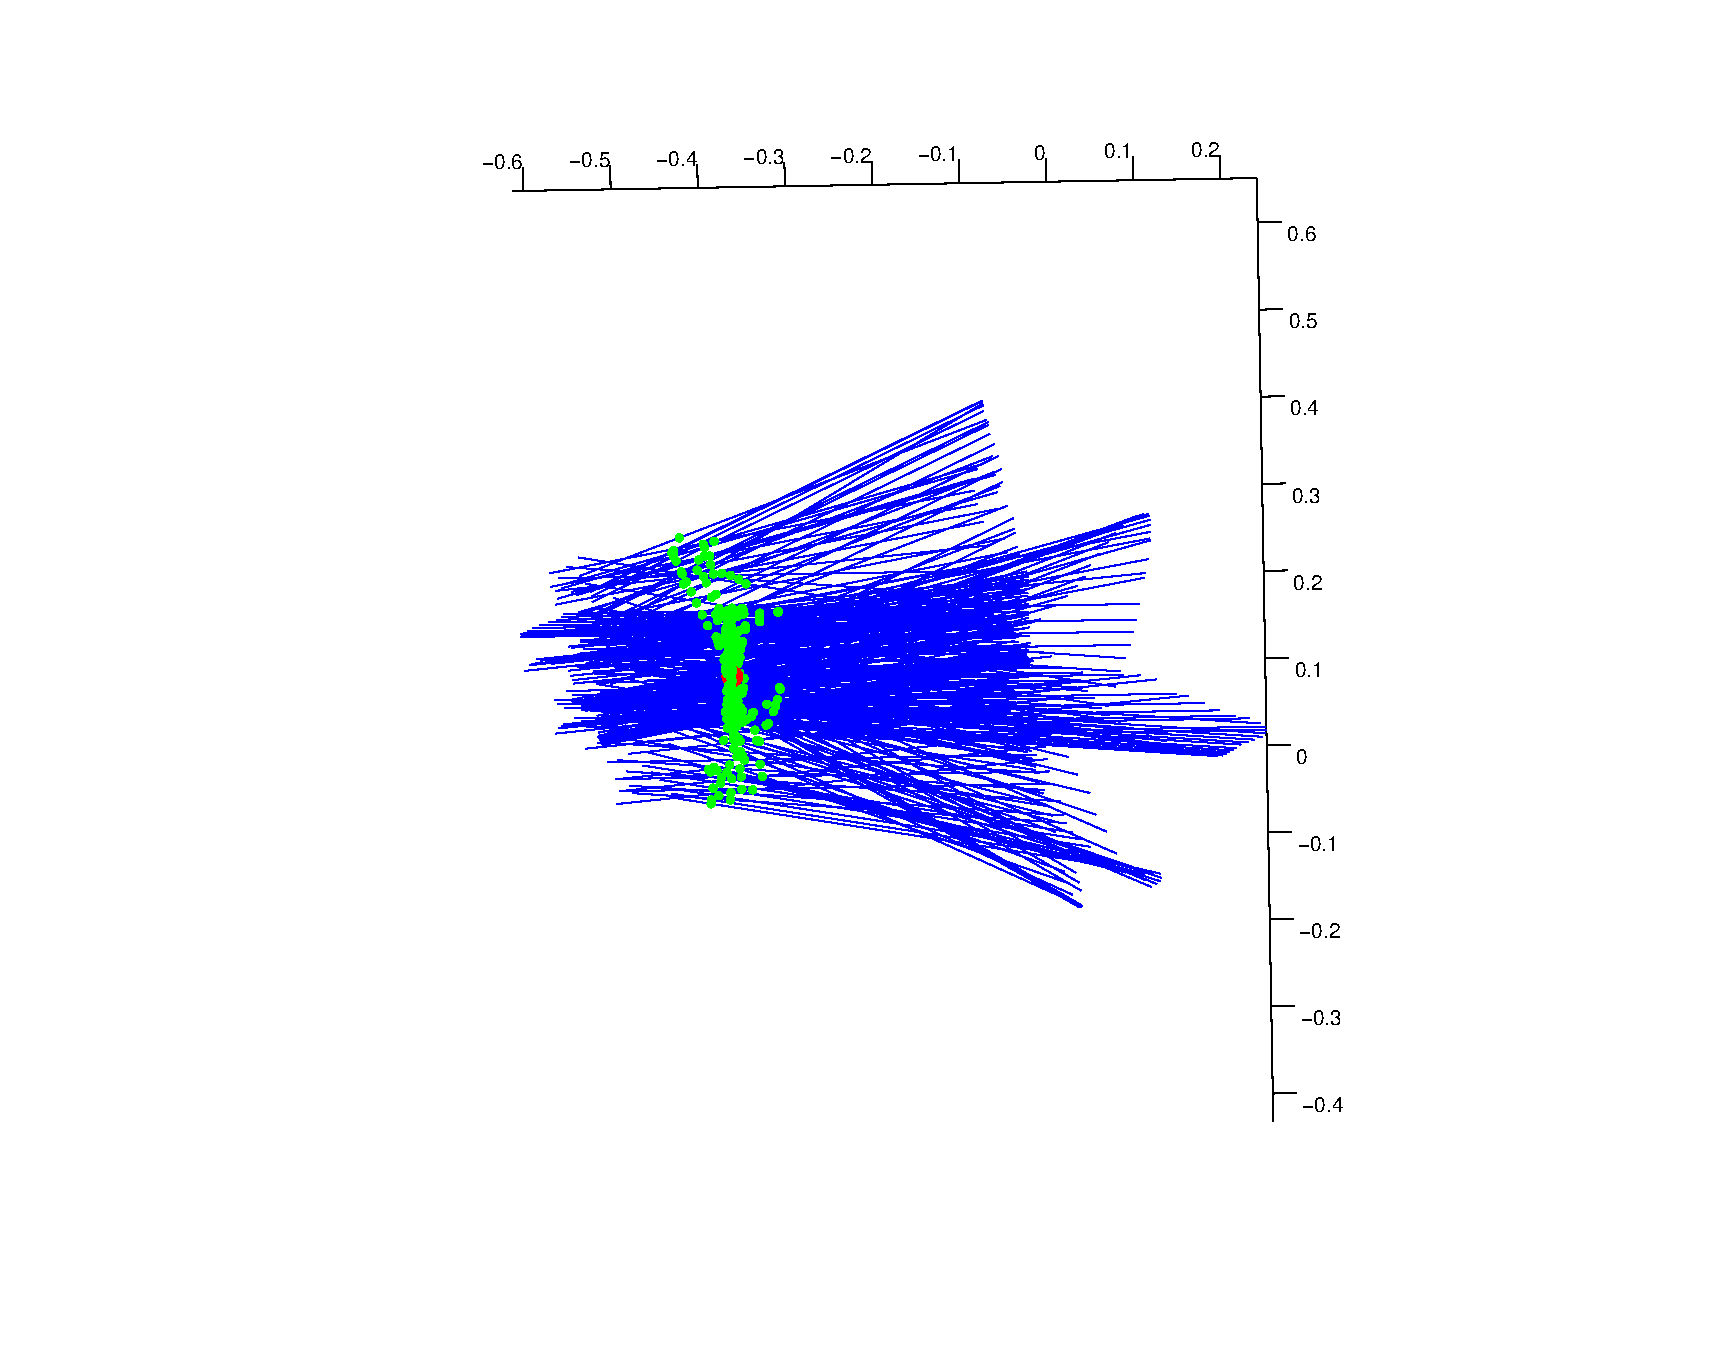
\includegraphics[width=1.1\linewidth]{./img/loc_calib_gauss.eps}
	\end{subfigure}
	\hfill
	\begin{subfigure}[b]{0.49\textwidth}
		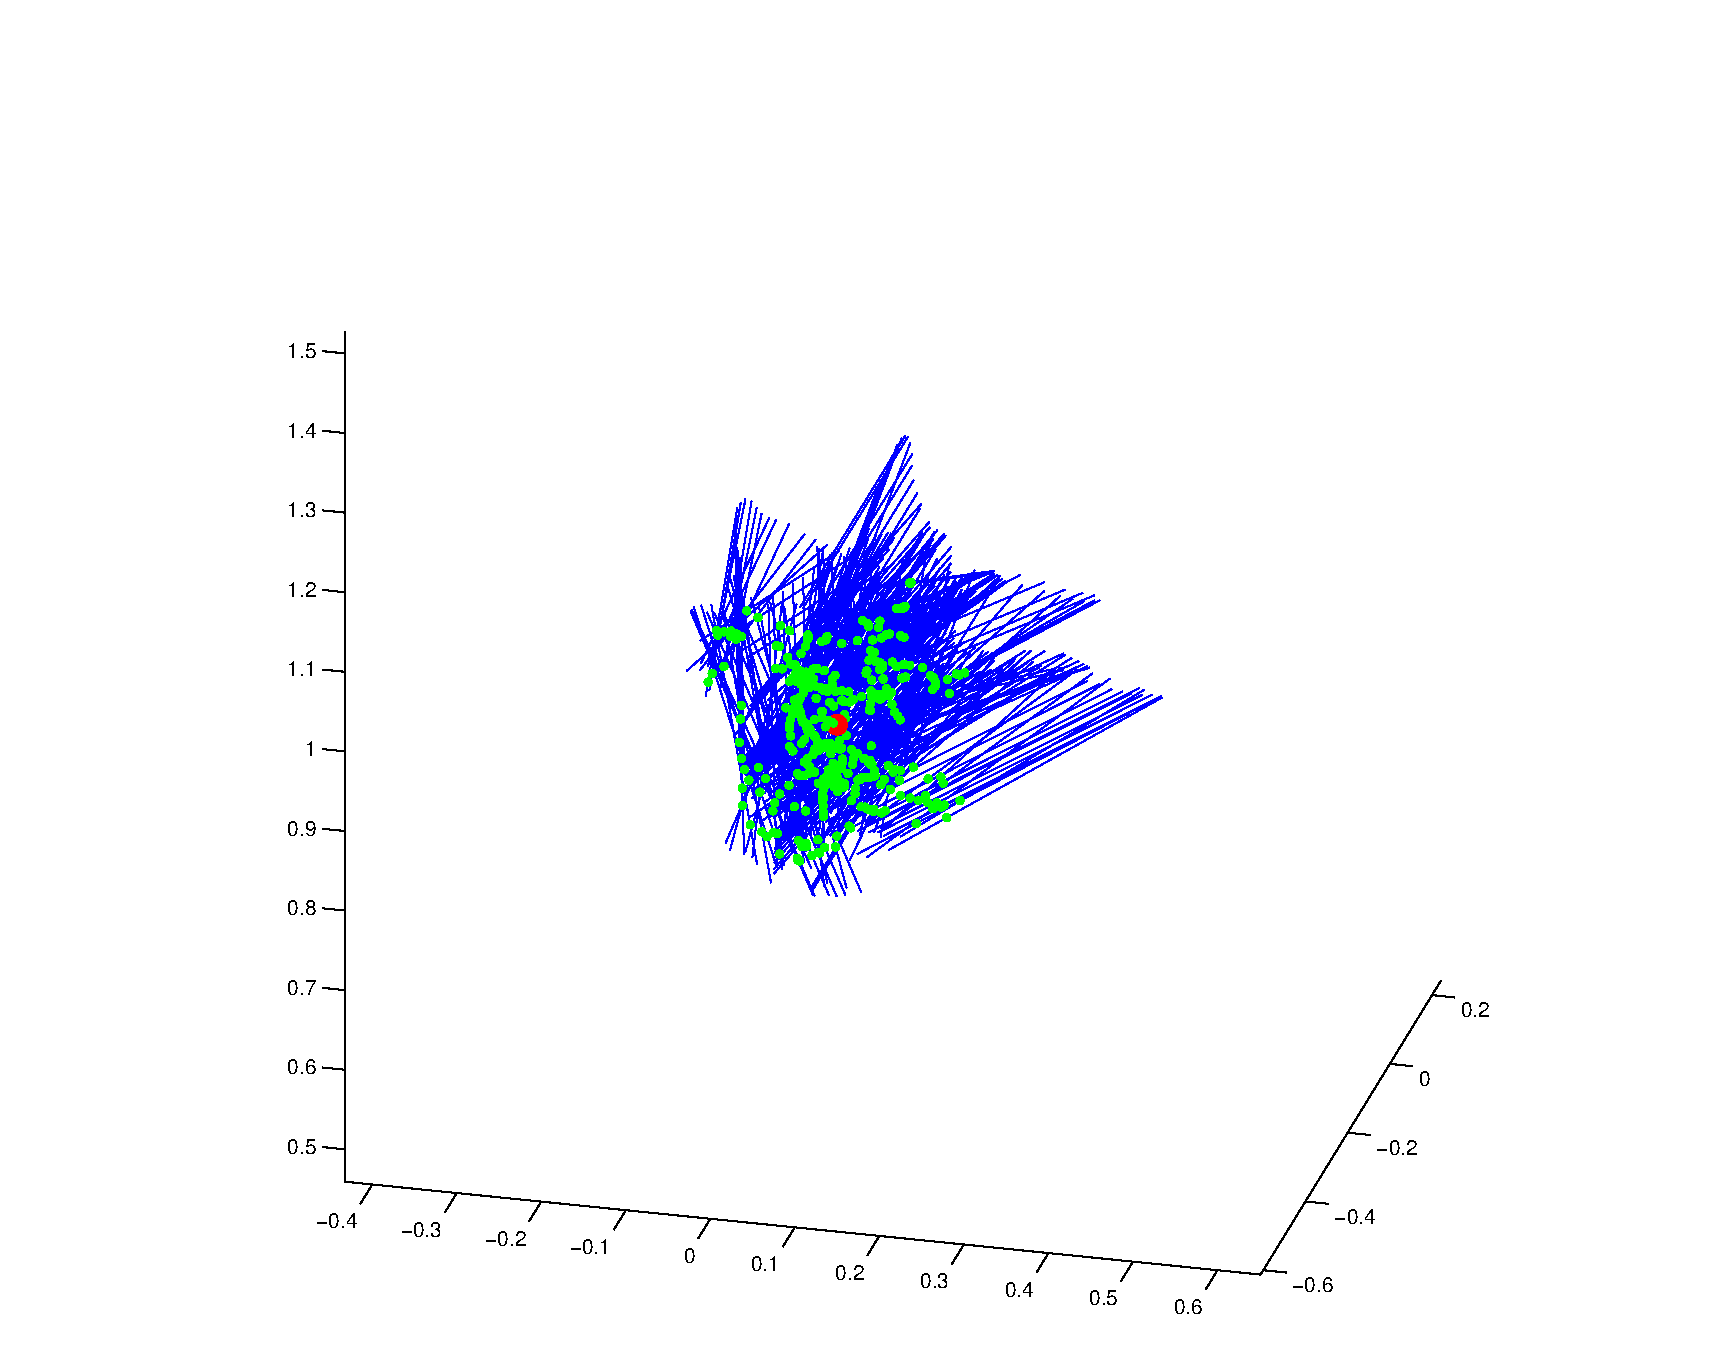
\includegraphics[width=1.1\linewidth]{./img/loc_calib_gauss_cross.eps}
	\end{subfigure}
	\caption{The Gaussian ellipsoid formed by finding the point of minimal sum of squared distances from all gaze lines.  Shown in red is the calculated point, shown in green are the closest point on each gaze line, shown in blue are the gaze lines.  In the left figure, the person doing the object location calibration is standing on the right, looking to the left.  The figure on the right shows the same plot rotated so the spread of the ellipsoid is seen more clearly.}
	\label{fig:locCalibResults}
\end{figure}

After this calibration for the objects of interest, we use a simple heuristic when identifying the object under gaze.  If gaze direction lies within x variance away from an object location mean, then this object is considered to be gazed at (x is a sensitivity parameter chosen manually).  If the gaze lies in two or more objects' vicinities, the object whose distance from gaze normalized by variance is less is chosen as the object under gaze.  If no objects are close to the gaze direction, the person is considered not looking at any object, i.e. idling.

\section{Discussion}
We have shown working modification of the KinFu algorithm that produces frontal head pose transformed color eye images.  However, due to limitation of time, the head tracking algorithm was not evaluated.  We did some preliminary testing with the Kinect video footages we have obtained of the child with ASD during his hand-washing trials.  However, because the Kinect camera was placed too close to the participant's face (due to limitation of space near the sink), and because the participant rocks back and forth quite rapidly, our algorithm could not track the participant's head motions well.  Thus, we were not able to build a head model from the footages, and thus further evaluation (building frontal head pose transformed color eye images) was impeded.

For future studies, we need to first ensure the head tracker we developed works with children with ASD.  To do this, we should characterize children with ASD's head movement during hand-washing with the robot, since some children with ASD exhibit rocking motions.  We should note the speed and range of motions.  We may need to reposition the Kinect camera further away from the child to make sure the child's head motions does not go out of camera's range.  Then we need to characterize our head tracker's capability and make sure it can handle children with ASD's head movements.  If the head movements of children with ASD are faster than the tracker can handle, we may consider decreasing the number of vertices in the head model mesh to increase frame rate.

After obtaining a head tracker that works with children with ASD, we can move on to implementing the eye tracker.  Eye tracking training images can be obtained by using the head tracker, doing the frontal pose transformation, and cropping the eye region using the EYEDIAP dataset.  Then the eye tracker can be implemented following the ALR method outlined previously.

For the future studies, we should evaluate the gaze (head plus eye) tracking accuracy for children with ASD.  One way to evaluate it is by letting children with ASD wear a commercially available gaze tracking headset that gives the ground truth of their gaze, and compare it with the gaze direction estimated by our head plus eye tracker.  However, if asking children with ASD to wear the obtrusive headset proves infeasible, then maybe a fun activity can be designed instead that asks children with ASD to look at a moving object (e.g. a ball) whose 3D position can be automatically estimated using Kinect, serving as ground truth.

Lastly, future studies should integrate the head and eye tracker with object under gaze estimator to fully realize the VFOA tracker -- tracking the object under gaze in real-time.  Robot behaviors responding to child's gaze should then be implemented.  A study evaluating the effectiveness of this child's gaze behavior dependent robot prompting on children with ASD's engagement, prompt compliance, and step completion during hand-washing should be conducted.
\chapter{Conclusion}
In this thesis, we aimed to investigate a new prompting agent, humanoid robot NAO, for COACH during the prompting of hand-washing steps to a child with ASD.  A Wizard of Oz (WoZ) study was conducted, and yielded promising results.  In addition, we further improved COACH by attempting to implement a Visual Focus of Attention (VFOA) tracker.  The thesis answers the hypotheses raised in the following way (the hypotheses are shown in bold):

\paragraph{The humanoid robot, NAO, is able to independently assist child with ASD through hand-washing, and child exhibits greater engagement level, higher prompt compliance\DIFdelbegin \DIFdel{rate}\DIFdelend , and better task completion when prompted by NAO than by parent.}
Through the WoZ study, we have seen that NAO was effective in facilitating task completion in both variety and quality of steps, approaching the level of effectiveness achieved by the parent, but not better.  Also, NAO had a low \DIFdelbegin \DIFdel{prompt compliance rate }\DIFdelend \DIFaddbegin \DIFadd{Complied Prompt Rate }\DIFaddend compared to the parent during the first phase when it was introduced, but through a training phase of joint prompting with the parent, NAO resulted in a higher \DIFdelbegin \DIFdel{prompt compliance rate }\DIFdelend \DIFaddbegin \DIFadd{Complied Prompt Rate }\DIFaddend than before, comparable to that of the parent's.  We attribute the improvements of the robot effectiveness to the training phase, though several confounding variables such as learning effects, fatigue, and robot control were discussed.  In whole, although we have not achieved totally independent assistance using NAO, we have shown that NAO has very good potential of achieving independent assistance, given a longer and more intense training phase.

\paragraph{Gestural, gaze, and verbal are the essential modes of interactions present in the hand-washing prompting scenario between child with ASD and the prompting agent NAO.}
The WoZ study revealed that verbal instructions and pointing gestures are essential for a prompting agent to assist our participant, who knows the execution of each hand-washing step, but needs reminders of which step to execute.  In cases the child did need demonstrations for a step, NAO's limited dexterity as well as the slower motion speed of the motion demonstrations made it less effective compared to that of the parent's.  In addition, when the child is not complying, the parent increased the severity of the prompts, which the robot should implement in the future.  In terms of gaze behaviors during interactions, our participant generally avoided looking at the prompting agent when he knew what to do, and tends to look at the parent more than NAO when seeking help.  The child's gaze behavior was a poor indication of engagement.  Lastly, detection and understanding of verbal feedbacks from the child may be useful in predicting the engagement of our participant.

\paragraph{Using 3DMM and ALR for estimating head pose and eye pose, and using the Kinect camera, a classification rate of more than 80\% is achieved for estimating child's VFOA on NAO, monitor screen, soap, towel, tap region, hands, and idling.}
We have successfully completed a head pose tracker using the Kinect camera by modifying the KinFu algorithm.  However, due to rapid head movements of the participant during hand-washing sessions, our head pose tracker was not successful in tracking his head.  Future improvements were suggested.  We have also implemented frontal pose transformation of the head image for eye region cropping.  But due to limitation of time, we did not implement the eye pose tracker using EYEDIAP dataset employing the ALR method.  Lastly, we implemented the object under gaze estimator.  In whole, we showed the feasibility of implementing the VFOA's three components (i.e. head pose tracker, eye pose tracker, object under gaze estimator), and described the steps for completing its implementation and evaluating its performance.

\section{Significance}
In conclusion, the thesis results suggest promising prospects of utilizing the humanoid robot, NAO, as a novel prompting agent to enhance COACH, and to fill the gap of in-vivo ATCs for teaching daily skills to children with ASD \DIFaddbegin \DIFadd{following the ABA framework}\DIFaddend .  Future investigations in regards to improving the child's engagement further through more creative design of the robot's appearance and behavior dynamics were suggested and explored.  One such improvement could come from implementing robot behaviors contingent to the VFOA of the child.

\section{\DIFdelbegin \DIFdel{Looking Back}\DIFdelend \DIFaddbegin \DIFadd{Thesis Process Reflections}\DIFaddend }
Looking back, there \DIFdelbegin \DIFdel{are several things we }\DIFdelend \DIFaddbegin \DIFadd{were several things the researcher }\DIFaddend could have done differently to have a more successful thesis.

\DIFdelbegin \DIFdel{Before the start of }\DIFdelend \DIFaddbegin \DIFadd{The biggest difficulty the researcher experienced was the lacking of intuitions in regards to children with ASD behaviors and how to design robot behaviors accordingly.  This difficulty stems from the researcher's lack of experience with children with ASD, and not having backgrounds in psychology, cognitive science, or behavior science.  This kind of problem is common in engineering design when the engineering team lacks expertise in the field application of the system.  To compensate, common strategies include iterative design process that includes experts and end users early and test the system prototypes frequently and rapidly so we can learn and succeed efficiently.  In the case of this thesis, }\DIFaddend the \DIFdelbegin \DIFdel{WoZ study, if the researcherhad a deeper and clearer understanding of qualitative analysis in case studies, the iterative qualitative data collection and analysis could have been carried more rigorously and efficiently, and possibly more yielded more results.  Starting the WoZ study earlier so we were less time limited would have been really nice, too.  That would mean longer training phase, and possibly yielding better results, even demonstrating the robot being as effective as the parent in prompting.  Also, having a few child alone hand-washing trials would be ideal, since we could use that opportunity to assess the child's habits and skills before starting the robot prompting trials, and less trials would be wasted in the researcher adjusting the robot prompting to the child's preference}\DIFdelend \DIFaddbegin \DIFadd{researcher had the resource of the committee, composed of expert researchers in the field of ATC for autism.  The researcher should have utilized this resource more, by seeking their knowledge and intuitions early in the design process.  Similarly, a more formal approach to this is setting up focus groups with parents, caregivers, therapists, and clinicians to review design prototypes early in the design process, which the researcher did not do, either.  Lastly, the researcher could have involved pilot testing the system with typically developing children first}\DIFaddend .  The researcher \DIFdelbegin \DIFdel{practiced controlling the robot to prompt adult volunteersthrough hand-washing during the study preparation phase, but the adults were very nice and all wanted to follow the robot.
Certain improvements were made to }\DIFdelend \DIFaddbegin \DIFadd{only tested with adult volunteers, which posed a bias in the test because the adult volunteers were all enthusiastic, lacking the opportunity to test scenarios of noncompliance from the user, especially due to lack of motivation and engagement.
}

\DIFadd{The researcher was not trained in qualitative research, and originally hoped to bypass the explorative case study (qualitative) stage, and directly conduct quantitative studies evaluating system efficacy.  Reflecting back, attempting to jump steps was progress hindering and led to inefficiency in learning what works in our design.  The explorative case study stage was a necessity because of the need to validate our assumptions and the need to gain intuitions on what measures and hypotheses are appropriate and meaningful for evaluative quantitative studies.  Furthermore, the research field of HRI for children with ASD is in its infancy.  It lacks theoretical frameworks that guide design decisions based on user behavior results.  In addition, }\DIFaddend the \DIFdelbegin \DIFdel{robot through this, but what we really needed was to test the robot for dealing with noncompliance behaviors, and testing the robot with normal children would have been much effective in this regard.
}\DIFdelend \DIFaddbegin \DIFadd{literatures in this field up to date offered very few descriptions on specific robot behaviors that are appropriate for facilitating both engagement and compliance from children with ASD.  All in all, hoping to produce successful results by skipping directly to a evaluative quantitative study with little grounding on our design decisions was a long shot, especially our use of humanoid robot to prompt children with ASD for daily living activity was the first research of its kind.  The researcher should have realized this from the start, and time could have been better allocated, investing less in learning quantitative research methods, not analyzing data for quantitative measures that yielded little significance, and better preparation for the case study and the qualitative research method.
}\DIFaddend 

\DIFdelbegin \DIFdel{During the study results analysis, we carried out quantitative analysis first, only relying on intuitions for what measures made sense to analyze.  After that , we carried out qualitative analysis and found better measures for quantitative analysis, and thus the quantitative analysis was revised in light of this.
Instead, if we did qualitative analysis first, our intuitions of what measures to be analyzed quantitatively }\DIFdelend \DIFaddbegin \DIFadd{Lastly for the clinical contribution, a larger portion of time should have been allocated for conducting the case study.  Our study results suggest the possibility that our participant would have demonstrated further improvement in robot compliance if the training phase (Phase C) was longer, and we would have greater confidence on the maintenance of such improvement if the robot testing phases (Phase B1 and B2) were longer, too.  In addition, the researcher wished the recruitment of subjects happened earlier, so that more than one subjects }\DIFaddend could have been \DIFdelbegin \DIFdel{founded in the qualitative results to begin with, saving time from much revisions.  }\DIFdelend \DIFaddbegin \DIFadd{recruited.  Our participant knew most of the hand-washing steps, thus although we showed improvement of compliance on our participant using the current design, the same design recommendations might not generalize to the population.  For a participant not knowing any hand-washing steps, the focus of robot prompts need to be shifted from step initiation to step motion teaching.  Finally, having a pre-test session where the child was observed to wash hands by himself with neither helps from the parent nor the robot would have added valuable grounding to our results.
}\DIFaddend 

For the technical contribution section of the thesis, instead of implementing \DIFaddbegin \DIFadd{three modules of the VFOA tracker (}\DIFaddend a head pose tracker, an eye pose tracker, and an object identification algorithm\DIFdelbegin \DIFdel{, we should decrease }\DIFdelend \DIFaddbegin \DIFadd{), the researcher should hvae decreased }\DIFaddend the scope to head tracking \DIFaddbegin \DIFadd{module }\DIFaddend only.  This way, \DIFdelbegin \DIFdel{we could have more time to properly evaluate the }\DIFdelend \DIFaddbegin \DIFadd{instead of running out of time investigating possible ways to implement the other two modules, the head tracking module could have been thoroughly investigated, including improving the eye cropping submodule to real-time and conducting proper evaluation of our module implementation's }\DIFaddend accuracy and robustness\DIFdelbegin \DIFdel{of the algorithm implemented.
}\DIFdelend \DIFaddbegin \DIFadd{.
}\DIFaddend 

\DIFaddbegin \DIFadd{In all, the researcher learned a lot of valuable lessons, both in regards to designing robot behaviors for children with ASD, and in regards to conducting qualitative and quantitative research.  Although many mistakes were made, the researcher is reminded of the Chinese phrase: ``Failure is the mother of success'', and hopes this thesis has been a good mother.
}\begin{appendices}
\chapter{\DIFadd{SRS Survey Result}}
\DIFadd{Choices for answers: 1 = Not True, 2 = Sometimes True, 3 = Often True, 4 = Almost Always True.
}\begin{longtable}{ | p{13cm} | l | }
	\hline
	\textbf{\DIFadd{Survey Question}}	&	\textbf{\DIFadd{Parent's Answer}}	\\	\hline	\hline		
	\DIFadd{1. Seems much more fidgety in social situations than when alone.	}&	\DIFadd{2	}\\	\hline
	\DIFadd{2. Expressions on his or her face don't match what he or she is saying.	}&	\DIFadd{2	}\\	\hline
	\DIFadd{3. Seems self-confident when interacting with others.	}&	\DIFadd{1	}\\	\hline
	\DIFadd{4. When under stress, he or she shows rigid or inflexible patterns of behavior that seem odd.	}&	\DIFadd{2	}\\	\hline
	\DIFadd{5. Doesn't recognize when other s are trying to take avantage of him or her.	}&	\DIFadd{4	}\\	\hline
	\DIFadd{6. Would rather be alone than with others.	}&	\DIFadd{4	}\\	\hline
	\DIFadd{7. Is aware of what others are thinking or feeling.	}&	\DIFadd{2	}\\	\hline
	\DIFadd{8. Behaves in ways that seem strage or bizarre.	}&	\DIFadd{3	}\\	\hline
	\DIFadd{9. Clings to adults, seems too dependent on them.	}&	\DIFadd{4	}\\	\hline
	\DIFadd{10. Takes things too literally and doesn't get the real meaning of a conversation.	}&	\DIFadd{3	}\\	\hline
	\DIFadd{11. Has good self-confidence.	}&	\DIFadd{2	}\\	\hline
	\DIFadd{12. Is able to communicate his or her feelings to others.	}&	\DIFadd{1	}\\	\hline
	\DIFadd{13. Is awkward in turn-taking interactions with peers (e.g., doesn't seem to understand the give-and-take of conversations).	}&	\DIFadd{1	}\\	\hline
	\DIFadd{14. Is not well coordinated.	}&	\DIFadd{2	}\\	\hline
	\DIFadd{15. Is able to understand the meaning of other people's tone of voice and facial expressions.	}&	\DIFadd{3	}\\	\hline
	\DIFadd{16. Avoids eye contact or has unusual eye contact	}&	\DIFadd{2	}\\	\hline
	\DIFadd{17. Recognizes wen something is unfair.	}&	\DIFadd{1	}\\	\hline
	\DIFadd{18. Has difficulty making friends, evn when trying his or her best.	}&	\DIFadd{4	}\\	\hline
	\DIFadd{19. Gets frustrated trying to get ideas across in conversations.	}&	\DIFadd{3	}\\	\hline
	\DIFadd{20. Shows unusual sensory interests (e.g., mouthing or spinning objects) or strange ways of playing with toys.	}&	\DIFadd{2	}\\	\hline
	\DIFadd{21. Is able to imitate others' actions.	}&	\DIFadd{3	}\\	\hline
	\DIFadd{22. Plays appropriately with children his or her age.	}&	\DIFadd{1	}\\	\hline
	\DIFadd{23. Does not join group actviities unless told to do so.	}&	\DIFadd{3	}\\	\hline
	\DIFadd{24. Has more difficulty than other children with changes in his or her routine.	}&	\DIFadd{2	}\\	\hline
	\DIFadd{25. Doesn't seem to mind being out of step with or ``not on the same wavelength'' as others.	}&	\DIFadd{3	}\\	\hline
	\DIFadd{26. Offers comfort to others when they are sad.	}&	\DIFadd{3	}\\	\hline
	\DIFadd{27. Avoids starting social interactions with peers or adults.	}&	\DIFadd{2	}\\	\hline
	\DIFadd{28. Thinks or talks about the same thing over and over.	}&	\DIFadd{3	}\\	\hline
	\DIFadd{29. Is regarded by other children as odd or weird.	}&	\DIFadd{3	}\\	\hline
	\DIFadd{30. Becomes upset in a situation with lots of things going on.	}&	\DIFadd{2	}\\	\hline
	\DIFadd{31. Can't get his or her mind off something once her or she starts thinking about it.	}&	\DIFadd{2	}\\	\hline
	\DIFadd{32. Has good personal hygiene.	}&	\DIFadd{3	}\\	\hline
	\DIFadd{33. Is socially awkward, even when he or she is trying to be polite.	}&	\DIFadd{3	}\\	\hline
	\DIFadd{34. Avoids people who want to be emotionally close to him or her.	}&	\DIFadd{3	}\\	\hline
	\DIFadd{35. Has troube keeping up with the flow of a normal conversation.	}&	\DIFadd{3	}\\	\hline
	\DIFadd{36. Has difficulty relating to adults.	}&	\DIFadd{2	}\\	\hline
	\DIFadd{37. Has difficulty relating to peers.	}&	\DIFadd{3	}\\	\hline
	\DIFadd{38. Responds appropriately to mood changes in others (e.g., when a friend's or playmate's mood changes from happy to sad).	}&	\DIFadd{2	}\\	\hline
	\DIFadd{39. Has an unusually narrow range of interests.	}&	\DIFadd{2	}\\	\hline
	\DIFadd{40. Is imaginative, good at pretending (without losing touch with reality).	}&	\DIFadd{1	}\\	\hline
	\DIFadd{41. Wanders aimlessly from one activity to another.	}&	\DIFadd{3	}\\	\hline
	\DIFadd{42. Seems overly sensitive to sounds, textures, or smells.	}&	\DIFadd{3	}\\	\hline
	\DIFadd{43. Separates easily from caregivers.	}&	\DIFadd{2	}\\	\hline
	\DIFadd{44. Doesn't understand how events relate to one another (cause and effect) the way other children his or her age do.	}&	\DIFadd{3	}\\	\hline
	\DIFadd{45. Focuses his or her attention to where others are looking or listening.	}&	\DIFadd{2	}\\	\hline
	\DIFadd{46. Has overly serious facial expressions.	}&	\DIFadd{2	}\\	\hline
	\DIFadd{47. Is too silly or laughs inappropriately.	}&	\DIFadd{2	}\\	\hline
	\DIFadd{48. Has a sense of humor, understands jokes.	}&	\DIFadd{2	}\\	\hline
	\DIFadd{49. Does extremely well at a few tasks, but does not do as well at most other tasks.	}&	\DIFadd{3	}\\	\hline
	\DIFadd{50. Has repetitive, odd behaviors such as hand flapping or rocking.	}&	\DIFadd{4	}\\	\hline
	\DIFadd{51. Has difficulty answering questions directly and ends up talking around the subject.	}&	\DIFadd{4	}\\	\hline
	\DIFadd{52. Knows when he or she is talking too loud or making too much noise.	}&	\DIFadd{1	}\\	\hline
	\DIFadd{53. Talks to people with an unusual tone of voice (e.g., talks like a robot ro like he or she is giving a lecture).	}&	\DIFadd{1	}\\	\hline
	\DIFadd{54. Seems to react to people as if they are objects.	}&	\DIFadd{2	}\\	\hline
	\DIFadd{55. Knows when he or she is too close to someone or is invading someone's space.	}&	\DIFadd{1	}\\	\hline
	\DIFadd{56. Walks in between two people who are talking.	}&	\DIFadd{3	}\\	\hline
	\DIFadd{57. Gets teased a lot.	}&	\DIFadd{2	}\\	\hline
	\DIFadd{58. Concentrates too much on parts of things rather than seeing the whole picture.  For example, if asked to describe what happened in a story, he or she may talk only about the kind of clothes the characters were wearing.	}&	\DIFadd{1	}\\	\hline
	\DIFadd{59. Is overly suspicious.	}&	\DIFadd{1	}\\	\hline
	\DIFadd{60. Is emotionally distant, doesn't show his or her feelings.	}&	\DIFadd{2	}\\	\hline
	\DIFadd{61. Is inflexible, has a hard time changing his or her mind.	}&	\DIFadd{2	}\\	\hline
	\DIFadd{62. Gives unusual or illogical reasons for doing things.	}&	\DIFadd{2	}\\	\hline
	\DIFadd{63. Touches others in an unusual way (e.g., he or she may touch someone just to make contact and then walk away without saying anything).	}&	\DIFadd{4	}\\	\hline
	\DIFadd{64. Is too tense in social settings.	}&	\DIFadd{3	}\\	\hline
	\DIFadd{65. Stares or gazes off into space.	}&	\DIFadd{4	}\\	\hline
\caption{\DIFadd{The SRS Survey Data}}
\label{tab:SRSSurveyData}
\end{longtable}

\chapter{\DIFadd{Post-Intervention Survey Result}}
\DIFadd{Choices for answers: Strongly Agree, Agree, Neither Agree nor Disagree, Disagree, Strongly Disagree.
}\begin{table}[H]
	\centering
	\begin{tabular}{ | p{12cm} | l | }
		\hline
		\textbf{\DIFaddFL{Survey Question}}	&	\textbf{\DIFaddFL{Parent's Answer}}	\\	\hline	\hline		
		\DIFaddFL{Hand-washing steps break down was appropriate	}&	\DIFaddFL{Strongly Agree	}\\	\hline
		\DIFaddFL{My child understood the verbal prompts	}&	\DIFaddFL{Agree	}\\	\hline
		\DIFaddFL{Robot's verbal prompts were appropriate	}&	\DIFaddFL{Strongly Agree	}\\	\hline
		\DIFaddFL{The prompt wordings were similar to mine	}&	\DIFaddFL{Strongly Agree	}\\	\hline
		\DIFaddFL{The prompt voice and tone were appropriate	}&	\DIFaddFL{Strongly Agree	}\\	\hline
		\DIFaddFL{The prompt wordings were easy to understand	}&	\DIFaddFL{Strongly Agree }\\	\hline
		\DIFaddFL{My child understood the gesture prompts	}&	\DIFaddFL{Strongly Agree	}\\	\hline
		\DIFaddFL{The gesture prompts were appropriate	}&	\DIFaddFL{Strongly Agree	}\\	\hline
		\DIFaddFL{The gesture prompts were easy to understand	}&	\DIFaddFL{Agree	}\\	\hline
		\DIFaddFL{The physical appearance of robot is aesthetically pleasing	}&	\DIFaddFL{Agree	}\\	\hline
		\DIFaddFL{The attention grabber gestures were appropriate	}&	\DIFaddFL{Strongly Agree	}\\	\hline
		\DIFaddFL{The verbal rewards were appropriate	}&	\DIFaddFL{Strongly Agree	}\\	\hline
		\DIFaddFL{The reward gestures were appropriate	}&	\DIFaddFL{Strongly Agree	}\\	\hline
		\DIFaddFL{The robot was effective in assisting my child through hand-washing	}&	\DIFaddFL{Strongly Agree	}\\	\hline
		\DIFaddFL{The robot motivated my child to wash hands	}&	\DIFaddFL{Strongly Agree	}\\	\hline
		\DIFaddFL{The robot was fun for my child to use	}&	\DIFaddFL{Strongly Agree	}\\	\hline
		\DIFaddFL{My child was confused by the robot	}&	\DIFaddFL{Disagree	}\\	\hline
		\DIFaddFL{I like the idea of a robot prompting my child	}&	\DIFaddFL{Strongly Agree	}\\	\hline
		\DIFaddFL{The robot is able to provide guidance as well as I can or better	}&	\DIFaddFL{Neither Agree or Disagree	}\\	\hline
		\DIFaddFL{I would want to own a robot like this one	}&	\DIFaddFL{Strongly Agree	}\\	\hline
	\end{tabular}
	\caption{\DIFaddFL{The Post-Intervention Survey Data}}
	\label{tab:PostInterventionSurveyData}
\end{table}

\end{appendices}

\DIFaddend %% This adds a line for the Bibliography in the Table of Contents.
\addcontentsline{toc}{chapter}{Bibliography}
%% *** Set the bibliography style. ***
%% (change according to your preference/requirements)
\bibliographystyle{plain}
%% *** Set the bibliography file. ***
%% ("thesis.bib" by default; change as needed)
\begin{thebibliography}{100}

\bibitem{abledata2010alpha}
{AbleData} alpha interactive language series—gator super sentences.
\newblock \url{http://www.abledata.com}.
\newblock Accessed: July 18, 2010.

\bibitem{autism2014facts}
{Autism Speaks Canada} facts and stats.
\newblock
  \url{http://www.autismservicesinc.com/pdf/Autism%20Speaks%20Canada%20Updated%20Facts%20and%20Stats.pdf}.
\newblock Accessed: June 20, 2015.

\bibitem{mackiev2010welcome}
{MacKiev.com} welcome to roger wagner’s hyperstudio.
\newblock \url{http://www.mackiev.com/hyperstudio}.
\newblock Accessed: September 27, 2010.

\bibitem{synapse2010the}
{Synapse Adaptive} the therapy tool that has people talking.
\newblock \url{http://www.synapseadaptive.com/edmark/prod/sv3}.
\newblock Accessed: July 20, 2010.

\bibitem{1997microsoft}
Microsoft powerpoint [computer software].
\newblock {\em Redmond, WA: Microsoft Corporation}, 1997–2003.

\bibitem{2005team}
Team up with timo: Animated learning tutor. [computer software].
\newblock {\em San Francisco, CA: Animated Speech Corporation}, 2005.

\bibitem{amberg2008expression}
Brian Amberg, Reinhard Knothe, and Thomas Vetter.
\newblock Expression invariant 3d face recognition with a morphable model.
\newblock In {\em Automatic Face \& Gesture Recognition, 2008. FG'08. 8th IEEE
  International Conference on}, pages 1--6. IEEE, 2008.

\DIFaddbegin \bibitem{ashton2001applications}
\DIFadd{Tamarah~M Ashton.
}\newblock \DIFadd{The applications of aba to technology: The discrete trial trainer.
}\newblock {\em \DIFadd{Journal of Special Education Technology}}\DIFadd{, 16(1):41, 2001.
}

\DIFaddend \bibitem{american2013diagnostic}
American~Psychiatric Association et~al.
\newblock {\em Diagnostic and Statistical Manual of Mental Disorders
  (DSM-5{\textregistered})}.
\newblock American Psychiatric Pub, 2013.

\bibitem{ayres2009acquisition}
Kevin~M Ayres, Amy Maguire, and Desiree McClimon.
\newblock Acquisition and generalization of chained tasks taught with computer
  based video instruction to children with autism.
\newblock {\em Education and Training in Developmental Disabilities},
  44(4):493, 2009.

\bibitem{baluja1994non}
Shumeet Baluja and Dean Pomerleau.
\newblock Non-intrusive gaze tracking using artificial neural networks.
\newblock Technical report, DTIC Document, 1994.

\bibitem{bandura1969principles}
Albert Bandura.
\newblock Principles of behavior modification.
\newblock 1969.

\bibitem{baoi2014prevalence}
J~Baoi.
\newblock Prevalence of autism spectrum disorder among children aged 8 years.
\newblock {\em MMWR Morb. Mortal. Wkly. Rep}, 63:1--21, 2014.

\bibitem{belkin2003laplacian}
Mikhail Belkin and Partha Niyogi.
\newblock Laplacian eigenmaps for dimensionality reduction and data
  representation.
\newblock {\em Neural computation}, 15(6):1373--1396, 2003.

\bibitem{bellini2007meta}
Scott Bellini and Jennifer Akullian.
\newblock A meta-analysis of video modeling and video self-modeling
  interventions for children and adolescents with autism spectrum disorders.
\newblock {\em Exceptional children}, 73(3):264--287, 2007.

\bibitem{bereznak2012video}
Sally Bereznak, Kevin~M Ayres, Linda~C Mechling, and Jennifer~L Alexander.
\newblock Video self-prompting and mobile technology to increase daily living
  and vocational independence for students with autism spectrum disorders.
\newblock {\em Journal of Developmental and Physical Disabilities},
  24(3):269--285, 2012.

\bibitem{bernard1999enhancing}
Vera Bernard-Opitz, N~Sriram, and Sharul Sapuan.
\newblock Enhancing vocal imitations in children with autism using the ibm
  speech viewer.
\newblock {\em Autism}, 3(2):131--147, 1999.

\bibitem{bertalmio2000image}
Marcelo Bertalmio, Guillermo Sapiro, Vincent Caselles, and Coloma Ballester.
\newblock Image inpainting.
\newblock In {\em Proceedings of the 27th annual conference on Computer
  graphics and interactive techniques}, pages 417--424. ACM
  Press/Addison-Wesley Publishing Co., 2000.

\bibitem{bhargava2013demonstration}
Shweta Bhargava, Srinivasan Janarthanam, Helen Hastie, Amol Deshmukh, Ruth
  Aylett, Lee Corrigan, and Ginevra Castellano.
\newblock Demonstration of the emote wizard of oz interface for empathic
  robotic tutors.
\newblock In {\em Proceedings of SIGdial}, 2013.

\bibitem{bimbrahw2012investigating}
Justin Bimbrahw, Jennifer Boger, and Alex Mihailidis.
\newblock Investigating the efficacy of a computerized prompting device to
  assist children with autism spectrum disorder with activities of daily
  living.
\newblock {\em Assistive Technology}, 24(4):286--298, 2012.

\bibitem{bogin2010steps}
J~Bogin, L~Sullivan, S~Rogers, A~Stabel, and D~Hatton.
\newblock Steps for implementation: Discrete trial training, 2010.

\bibitem{bondy1994picture}
Andrew~S Bondy and Lori~A Frost.
\newblock The picture exchange communication system.
\newblock {\em Focus on Autism and Other Developmental Disabilities},
  9(3):1--19, 1994.

\bibitem{bosseler2003development}
Alexis Bosseler and Dominic~W Massaro.
\newblock Development and evaluation of a computer-animated tutor for
  vocabulary and language learning in children with autism.
\newblock {\em Journal of autism and developmental disorders}, 33(6):653--672,
  2003.

\bibitem{buggey2005video}
Tom Buggey.
\newblock Video self-modeling applications with students with autism spectrum
  disorder in a small private school setting.
\newblock {\em Focus on autism and other developmental disabilities},
  20(1):52--63, 2005.

\bibitem{buggey1999training}
Tom Buggey, Kristina Toombs, Pia Gardener, and Michele Cervetti.
\newblock Training responding behaviors in students with autism using
  videotaped self-modeling.
\newblock {\em Journal of Positive Behavior Interventions}, 1(4):205--214,
  1999.

\bibitem{case2008evidence}
Jane Case-Smith and Marian Arbesman.
\newblock Evidence-based review of interventions for autism used in or of
  relevance to occupational therapy.
\newblock {\em American Journal of Occupational Therapy}, 62(4):416--429, 2008.

\DIFaddbegin \bibitem{chin2000teaching}
\DIFadd{Hsiao~Yun Chin and Vera Bernard-Opitz.
}\newblock \DIFadd{Teaching conversational skills to children with autism: Effect on the
  development of a theory of mind.
}\newblock {\em \DIFadd{Journal of Autism and Developmental Disorders}}\DIFadd{, 30(6):569--583,
  2000.
}

\DIFaddend \bibitem{cohen2006early}
Howard Cohen, Mila Amerine-Dickens, and Tristram Smith.
\newblock Early intensive behavioral treatment: Replication of the ucla model
  in a community setting.
\newblock {\em Journal of Developmental \& Behavioral Pediatrics},
  27(2):S145--S155, 2006.

\bibitem{coleman2005using}
Mari~Beth Coleman-Martin, Kathryn~Wolff Heller, David~F Cihak, and Kathryn~L
  Irvine.
\newblock Using computer-assisted instruction and the nonverbal reading
  approach to teach word identification.
\newblock {\em Focus on Autism and Other Developmental Disabilities},
  20(2):80--90, 2005.

\bibitem{colombo1999real}
Carlo Colombo and Alberto Del~Bimbo.
\newblock Real-time head tracking from the deformation of eye contours using a
  piecewise affine camera.
\newblock {\em Pattern Recognition Letters}, 20(7):721--730, 1999.

\bibitem{constantino2002social}
John~N Constantino and Christian~P Gruber.
\newblock The social responsiveness scale.
\newblock {\em Los Angeles: Western Psychological Services}, 2002.

\bibitem{dautenhahn2004towards}
Kerstin Dautenhahn and Iain Werry.
\newblock Towards interactive robots in autism therapy: Background, motivation
  and challenges.
\newblock {\em Pragmatics \& Cognition}, 12(1):1--35, 2004.

\bibitem{diehl2012clinical}
Joshua~J Diehl, Lauren~M Schmitt, Michael Villano, and Charles~R Crowell.
\newblock The clinical use of robots for individuals with autism spectrum
  disorders: A critical review.
\newblock {\em Research in autism spectrum disorders}, 6(1):249--262, 2012.

\bibitem{duquette2008exploring}
Audrey Duquette, Fran{\c{c}}ois Michaud, and Henri Mercier.
\newblock Exploring the use of a mobile robot as an imitation agent with
  children with low-functioning autism.
\newblock {\em Autonomous Robots}, 24(2):147--157, 2008.

\DIFaddbegin \bibitem{eldevik2009meta}
\DIFadd{Sigmund Eldevik, Richard~P Hastings, J~Carl Hughes, Erik Jahr, Svein Eikeseth,
  and Scott Cross.
}\newblock \DIFadd{Meta-analysis of early intensive behavioral intervention for children
  with autism.
}\newblock {\em \DIFadd{Journal of Clinical Child \& Adolescent Psychology}}\DIFadd{,
  38(3):439--450, 2009.
}

\bibitem{farley2009twenty}
\DIFadd{Megan~A Farley, William~M McMahon, Eric Fombonne, William~R Jenson, Judith
  Miller, Michael Gardner, Heidi Block, Carmen~B Pingree, Edward~R Ritvo,
  Riva~Arielle Ritvo, et~al.
}\newblock \DIFadd{Twenty-year outcome for individuals with autism and average or
  near-average cognitive abilities.
}\newblock {\em \DIFadd{Autism Research}}\DIFadd{, 2(2):109--118, 2009.
}

\DIFaddend \bibitem{feil2005defining}
David Feil-Seifer and Maja~J Mataric.
\newblock Defining socially assistive robotics.
\newblock In {\em Rehabilitation Robotics, 2005. ICORR 2005. 9th International
  Conference on}, pages 465--468. IEEE, 2005.

\bibitem{feil2009toward}
David Feil-Seifer and Maja~J Matari{\'c}.
\newblock Toward socially assistive robotics for augmenting interventions for
  children with autism spectrum disorders.
\newblock In {\em Experimental robotics}, pages 201--210. Springer, 2009.

\bibitem{fong2003survey}
Terrence Fong, Illah Nourbakhsh, and Kerstin Dautenhahn.
\newblock A survey of socially interactive robots.
\newblock {\em Robotics and autonomous systems}, 42(3):143--166, 2003.

\bibitem{foxx1982decreasing}
Richard~M Foxx.
\newblock {\em Decreasing behaviors of severely retarded and autistic persons}.
\newblock Research Press, 1982.

\bibitem{foxx2008applied}
Richard~M Foxx.
\newblock Applied behavior analysis treatment of autism: The state of the art.
\newblock {\em Child and adolescent psychiatric clinics of North America},
  17(4):821--834, 2008.

\bibitem{francis2005autism}
K~Francis.
\newblock Autism interventions: a critical update.
\newblock {\em Developmental Medicine \& Child Neurology}, 47(7):493--499,
  2005.

\bibitem{frank2004assistive}
Edmund Frank~Lopresti, Alex Mihailidis, and Ned Kirsch.
\newblock Assistive technology for cognitive rehabilitation: State of the art.
\newblock {\em Neuropsychological rehabilitation}, 14(1-2):5--39, 2004.

\bibitem{funes2012gaze}
Kenneth~Alberto Funes~Mora and J~Odobez.
\newblock Gaze estimation from multimodal kinect data.
\newblock In {\em Computer Vision and Pattern Recognition Workshops (CVPRW),
  2012 IEEE Computer Society Conference on}, pages 25--30. IEEE, 2012.

\bibitem{funes2013person}
Kenneth~Alberto Funes~Mora and Jean-Marc Odobez.
\newblock Person independent 3d gaze estimation from remote rgb-d cameras.
\newblock In {\em International Conference on Image Processing}, number
  EPFL-CONF-192423. IEEE, 2013.

\bibitem{ganz2012meta}
Jennifer~B Ganz, John~L Davis, Emily~M Lund, Fara~D Goodwyn, and Richard~L
  Simpson.
\newblock Meta-analysis of pecs with individuals with asd: Investigation of
  targeted versus non-targeted outcomes, participant characteristics, and
  implementation phase.
\newblock {\em Research in developmental disabilities}, 33(2):406--418, 2012.

\bibitem{ganz2012metab}
Jennifer~B Ganz, Theresa~L Earles-Vollrath, Amy~K Heath, Richard~I Parker,
  Mandy~J Rispoli, and Jaime~B Duran.
\newblock A meta-analysis of single case research studies on aided augmentative
  and alternative communication systems with individuals with autism spectrum
  disorders.
\newblock {\em Journal of autism and developmental disorders}, 42(1):60--74,
  2012.

\bibitem{ganz2013moderation}
Jennifer~B Ganz, Mandy~J Rispoli, Rose~Ann Mason, and Ee~Rea Hong.
\newblock Moderation of effects of aac based on setting and types of aided aac
  on outcome variables: An aggregate study of single-case research with
  individuals with asd.
\newblock {\em Developmental neurorehabilitation}, 17(3):184--192, 2013.

\bibitem{goldsmith2004use}
Tina~R Goldsmith and Linda~A LeBlanc.
\newblock Use of technology in interventions for children with autism.
\newblock {\em Journal of Early and Intensive Behavior Intervention}, 1(2):166,
  2004.

\bibitem{goodrich2007human}
Michael~A Goodrich and Alan~C Schultz.
\newblock Human-robot interaction: a survey.
\newblock {\em Foundations and trends in human-computer interaction},
  1(3):203--275, 2007.

\bibitem{graetz2006show}
Janet~E Graetz, Margo~A Mastropieri, and Thomas~E Scruggs.
\newblock Show time using video self-modeling to decrease inappropriate
  behavior.
\newblock {\em Teaching exceptional children}, 38(5):43--48, 2006.

\bibitem{hansen2010eye}
Dan~Witzner Hansen and Qiang Ji.
\newblock In the eye of the beholder: A survey of models for eyes and gaze.
\newblock {\em Pattern Analysis and Machine Intelligence, IEEE Transactions
  on}, 32(3):478--500, 2010.

\bibitem{heimann1995increasing}
Mikael Heimann, Keith~E Nelson, Tomas Tjus, and Christopher Gillberg.
\newblock Increasing reading and communication skills in children with autism
  through an interactive multimedia computer program.
\newblock {\em Journal of autism and developmental disorders}, 25(5):459--480,
  1995.

\bibitem{herrera2012joint}
C~Herrera, Juho Kannala, Janne Heikkil{\"a}, et~al.
\newblock Joint depth and color camera calibration with distortion correction.
\newblock {\em Pattern Analysis and Machine Intelligence, IEEE Transactions
  on}, 34(10):2058--2064, 2012.

\bibitem{hetzroni2005logos}
Orit~E Hetzroni and Uri Shalem.
\newblock From logos to orthographic symbols: A multilevel fading computer
  program for teaching nonverbal children with autism.
\newblock {\em Focus on Autism and Other Developmental Disabilities},
  20(4):201--212, 2005.

\bibitem{hetzroni2004effects}
Orit~E Hetzroni and Juman Tannous.
\newblock Effects of a computer-based intervention program on the communicative
  functions of children with autism.
\newblock {\em Journal of autism and developmental disorders}, 34(2):95--113,
  2004.

\bibitem{hine2006using}
Jeffrey~F Hine and Mark Wolery.
\newblock Using point-of-view video modeling to teach play to preschoolers with
  autism.
\newblock {\em Topics in Early Childhood Special Education}, 26(2):83--93,
  2006.

\bibitem{hitchcock2003video}
Caryl~H Hitchcock, Peter~W Dowrick, and Mary~Anne Prater.
\newblock Video self-modeling intervention in school-based settings a review.
\newblock {\em Remedial and Special Education}, 24(1):36--45, 2003.

\DIFaddbegin \bibitem{hojat2004visitor}
\DIFadd{Mohammadreza Hojat and Gang Xu.
}\newblock \DIFadd{A visitor's guide to effect sizes--statistical significance versus
  practical (clinical) importance of research findings.
}\newblock {\em \DIFadd{Advances in health sciences education}}\DIFadd{, 9(3):241--249, 2004.
}

\bibitem{howard2005comparison}
\DIFadd{Jane~S Howard, Coleen~R Sparkman, Howard~G Cohen, Gina Green, and Harold
  Stanislaw.
}\newblock \DIFadd{A comparison of intensive behavior analytic and eclectic treatments
  for young children with autism.
}\newblock {\em \DIFadd{Research in developmental disabilities}}\DIFadd{, 26(4):359--383, 2005.
}

\DIFaddend \bibitem{howlin2003outcome}
Patricia Howlin.
\newblock Outcome in high-functioning adults with autism with and without early
  language delays: implications for the differentiation between autism and
  asperger syndrome.
\newblock {\em Journal of autism and developmental disorders}, 33(1):3--13,
  2003.

\bibitem{howlin2009systematic}
Patricia Howlin, Iliana Magiati, and Tony Charman.
\newblock Systematic review of early intensive behavioral interventions for
  children with autism.
\newblock {\em Journal Information}, 114(1), 2009.

\bibitem{hutcherson2004computer}
Karen Hutcherson, John Langone, Kevin Ayres, and Tom Clees.
\newblock Computer assisted instruction to teach item selection in grocery
  stores: An assessment of acquisition and generalization.
\newblock {\em Journal of Special Education Technology}, 19(4):33--42, 2004.

\bibitem{kagohara2013using}
Debora~M Kagohara, Larah van~der Meer, Sathiyaprakash Ramdoss, Mark~F
  O’Reilly, Giulio~E Lancioni, Tonya~N Davis, Mandy Rispoli, Russell Lang,
  Peter~B Marschik, Dean Sutherland, et~al.
\newblock Using ipods{\textregistered} and ipads{\textregistered} in teaching
  programs for individuals with developmental disabilities: A systematic
  review.
\newblock {\em Research in developmental disabilities}, 34(1):147--156, 2013.

\DIFaddbegin \bibitem{keenan2014autism}
\DIFadd{Mickey Keenan, Karola Dillenburger, Hanns~R}{\DIFadd{\"u}}\DIFadd{diger R}{\DIFadd{\"o}}\DIFadd{ttgers, Katerina
  Dounavi, Sigrs-Ortega, Lise Roll-Pettersson, and
  Neil Martin.
}\newblock \DIFadd{Autism and aba: The gulf between north america and europe.
}\newblock {\em \DIFadd{Review Journal of Autism and Developmental Disorders}}\DIFadd{,
  2(2):167--183, 2014.
}

\DIFaddend \bibitem{kim2001second}
Sunyonga Kim and Masakazu Kojima.
\newblock Second order cone programming relaxation of nonconvex quadratic
  optimization problems.
\newblock {\em Optimization Methods and Software}, 15(3-4):201--224, 2001.

\DIFaddbegin \bibitem{koegel2003teaching}
\DIFadd{Lynn~Kern Koegel, Cynthia~M Carter, and Robert~L Koegel.
}\newblock \DIFadd{Teaching children with autism self-initiations as a pivotal response.
}\newblock {\em \DIFadd{Topics in Language Disorders}}\DIFadd{, 23(2):134--145, 2003.
}

\DIFaddend \bibitem{kozima2005interactive}
Hideki Kozima, Cocoro Nakagawa, and Yuriko Yasuda.
\newblock Interactive robots for communication-care: A case-study in autism
  therapy.
\newblock In {\em Robot and Human Interactive Communication, 2005. ROMAN 2005.
  IEEE International Workshop on}, pages 341--346. IEEE, 2005.

\bibitem{kruger2002gabor}
Volker Kr{\"u}ger and Gerald Sommer.
\newblock Gabor wavelet networks for efficient head pose estimation.
\newblock {\em Image and vision computing}, 20(9):665--672, 2002.

\bibitem{lang2014assistive}
Russell Lang, Sathiyaprakash Ramdoss, Tracy Raulston, Amarie Carnet, Jeff
  Sigafoos, Robert Didden, Dennis Moore, and Mark~F O’Reilly.
\newblock Assistive technology for people with autism spectrum disorders.
\newblock In {\em Assistive Technologies for People with Diverse Abilities},
  pages 157--190. Springer, 2014.

\DIFaddbegin \bibitem{lathan2007using}
\DIFadd{Corinna Lathan, Katharina Boser, Charlotte Safos, Cathy Frentz, and Kaitlin
  Powers.
}\newblock \DIFadd{Using cosmo’s learning system (cls) with children with autism.
}\newblock \DIFadd{In }{\em \DIFadd{Proceedings of the International Conference on
  Technology-Based Learning with Disabilities}}\DIFadd{, pages 37--47. Citeseer, 2007.
}

\DIFaddend \bibitem{li2000support}
Yongmin Li, Shaogang Gong, and Heather Liddell.
\newblock Support vector regression and classification based multi-view face
  detection and recognition.
\newblock In {\em Automatic Face and Gesture Recognition, 2000. Proceedings.
  Fourth IEEE International Conference on}, pages 300--305. IEEE, 2000.

\bibitem{liss2001predictors}
Miriam Liss, Brian Harel, Deborah Fein, Doris Allen, Michelle Dunn, Carl
  Feinstein, Robin Morris, Lynn Waterhouse, and Isabel Rapin.
\newblock Predictors and correlates of adaptive functioning in children with
  developmental disorders.
\newblock {\em Journal of autism and developmental disorders}, 31(2):219--230,
  2001.

\bibitem{lovaas1987behavioral}
O~Ivar Lovaas.
\newblock Behavioral treatment and normal educational and intellectual
  functioning in young autistic children.
\newblock {\em Journal of consulting and clinical psychology}, 55(1):3, 1987.

\bibitem{lovaas1979stimulus}
O~Ivar Lovaas, Robert~L Koegel, and Laura Schreibman.
\newblock Stimulus overselectivity in autism: A review of research.
\newblock {\em Psychological bulletin}, 86(6):1236, 1979.

\bibitem{low2004linear}
Kok-Lim Low.
\newblock Linear least-squares optimization for point-to-plane icp surface
  registration.
\newblock {\em Chapel Hill, University of North Carolina}, 2004.

\bibitem{lu2011inferring}
Feng Lu, Yusuke Sugano, Takahiro Okabe, and Yoichi Sato.
\newblock Inferring human gaze from appearance via adaptive linear regression.
\newblock In {\em Computer Vision (ICCV), 2011 IEEE International Conference
  on}, pages 153--160. IEEE, 2011.

\bibitem{massaro2006read}
Dominic~W Massaro and Alexis Bosseler.
\newblock Read my lips the importance of the face in a computer-animated tutor
  for vocabulary learning by children with autism.
\newblock {\em Autism}, 10(5):495--510, 2006.

\bibitem{mataric2005role}
Maja~J Mataric.
\newblock The role of embodiment in assistive interactive robotics for the
  elderly.
\newblock In {\em AAAI fall symposium on caring machines: AI for the elderly,
  Arlington, VA}, 2005.

\DIFaddbegin \bibitem{mcgee1986extension}
\DIFadd{Gail~G McGee, Patricia~J Krantz, and Lynn~E McClannahan.
}\newblock \DIFadd{An extension of incidental teaching procedures to reading instruction
  for autistic children.
}\newblock {\em \DIFadd{Journal of Applied Behavior Analysis}}\DIFadd{, 19(2):147--157, 1986.
}

\DIFaddend \bibitem{mechling2010computer}
Linda Mechling and Eileen O'Brien.
\newblock Computer-based video instruction to teach students with intellectual
  disabilities to use public bus transportation.
\newblock {\em Education and Training in Autism and Developmental
  Disabilities}, pages 230--241, 2010.

\bibitem{merriam2014qualitative}
Sharan~B Merriam.
\newblock {\em Qualitative research: A guide to design and implementation}.
\newblock John Wiley \& Sons, 2014.

\bibitem{mihailidis2008coach}
Alex Mihailidis, Jennifer~N Boger, Tammy Craig, and Jesse Hoey.
\newblock The coach prompting system to assist older adults with dementia
  through handwashing: An efficacy study.
\newblock {\em BMC geriatrics}, 8(1):28, 2008.

\bibitem{mirenda2001autism}
Pat Mirenda.
\newblock Autism, augmentative communication, and assistive technology what do
  we really know?
\newblock {\em Focus on Autism and Other Developmental Disabilities},
  16(3):141--151, 2001.

\bibitem{moore2000brief}
Monique Moore and Sandra Calvert.
\newblock Brief report: Vocabulary acquisition for children with autism:
  Teacher or computer instruction.
\newblock {\em Journal of autism and developmental disorders}, 30(4):359--362,
  2000.

\bibitem{mora2014eyediap}
Kenneth Alberto~Funes Mora, Florent Monay, and Jean-Marc Odobez.
\newblock Eyediap: a database for the development and evaluation of gaze
  estimation algorithms from rgb and rgb-d cameras.
\newblock In {\em Proceedings of the Symposium on Eye Tracking Research and
  Applications}, pages 255--258. ACM, 2014.

\bibitem{murphy2009head}
Erik Murphy-Chutorian and Mohan~M Trivedi.
\newblock Head pose estimation in computer vision: A survey.
\newblock {\em Pattern Analysis and Machine Intelligence, IEEE Transactions
  on}, 31(4):607--626, 2009.

\bibitem{newcombe2011kinectfusion}
Richard~A Newcombe, Shahram Izadi, Otmar Hilliges, David Molyneaux, David Kim,
  Andrew~J Davison, Pushmeet Kohi, Jamie Shotton, Steve Hodges, and Andrew
  Fitzgibbon.
\newblock Kinectfusion: Real-time dense surface mapping and tracking.
\newblock In {\em Mixed and augmented reality (ISMAR), 2011 10th IEEE
  international symposium on}, pages 127--136. IEEE, 2011.

\DIFaddbegin \bibitem{palmen2013behavioral}
\DIFadd{Anna Maria Josephina~Wilhelmina Palmen.
}\newblock {\em \DIFadd{Behavioral interventions in adolescents and young adults with
  high-functioning ASD: Improvement, generalization, and maintenance of
  adaptive skills}}\DIFadd{.
}\newblock \DIFadd{UB Nijmegen }[\DIFadd{Host}]\DIFadd{, 2013.
}

\DIFaddend \bibitem{parsons1993effect}
Carl~L Parsons and Diane La~Sorte.
\newblock The effect of computers with synthesized speech and no speech on the
  spontaneous communication of children with autism.
\newblock {\em Australian Journal of Human Communication Disorders},
  21(1):12--31, 1993.

\bibitem{paysan20093d}
Pascal Paysan, Reinhard Knothe, Brian Amberg, Sami Romdhani, and Thomas Vetter.
\newblock A 3d face model for pose and illumination invariant face recognition.
\newblock In {\em Advanced Video and Signal Based Surveillance, 2009. AVSS'09.
  Sixth IEEE International Conference On}, pages 296--301. IEEE, 2009.

\DIFaddbegin \bibitem{peters2011meta}
\DIFadd{Nienke Peters-Scheffer, Robert Didden, Hubert Korzilius, and Peter Sturmey.
}\newblock \DIFadd{A meta-analytic study on the effectiveness of comprehensive aba-based
  early intervention programs for children with autism spectrum disorders.
}\newblock {\em \DIFadd{Research in Autism Spectrum Disorders}}\DIFadd{, 5(1):60--69, 2011.
}

\bibitem{picardo2014towards}
\DIFadd{Valerie Picardo, Samuel Metson, Rashina Hoda, Robert Amor, Angela
  Arnold-Saritepe, Rebecca Sharp, and Denys Brand.
}\newblock \DIFadd{Towards designing assistive software applications for discrete trial
  training.
}\newblock \DIFadd{In }{\em \DIFadd{Companion Proceedings of the 36th International Conference on
  Software Engineering}}\DIFadd{, pages 622--623. ACM, 2014.
}

\DIFaddend \bibitem{pierno2008robotic}
Andrea~C Pierno, Morena Mari, Dean Lusher, and Umberto Castiello.
\newblock Robotic movement elicits visuomotor priming in children with autism.
\newblock {\em Neuropsychologia}, 46(2):448--454, 2008.

\bibitem{pirovano2011kinfu}
M.~Pirovano.
\newblock Kinfu – an open-source implementation of kinect fusion + case
  study: Implementing a 3d scanner with pcl.
\newblock {\em 3D Structure from Visual Motion}, 2011/2012.

\bibitem{preston2009review}
Deborah Preston and Mark Carter.
\newblock A review of the efficacy of the picture exchange communication system
  intervention.
\newblock {\em Journal of autism and developmental disorders},
  39(10):1471--1486, 2009.

\DIFaddbegin \bibitem{rajendran2007cognitive}
\DIFadd{Gnanathusharan Rajendran and Peter Mitchell.
}\newblock \DIFadd{Cognitive theories of autism.
}\newblock {\em \DIFadd{Developmental Review}}\DIFadd{, 27(2):224--260, 2007.
}

\DIFaddend \bibitem{ramdoss2011use}
Sathiyaprakash Ramdoss, Russell Lang, Austin Mulloy, Jessica Franco, Mark
  O’Reilly, Robert Didden, and Giulio Lancioni.
\newblock Use of computer-based interventions to teach communication skills to
  children with autism spectrum disorders: A systematic review.
\newblock {\em Journal of Behavioral Education}, 20(1):55--76, 2011.

\bibitem{ramdoss2012computer}
Sathiyaprakash Ramdoss, Wendy Machalicek, Mandy Rispoli, Austin Mulloy, Russell
  Lang, and Mark O'Reilly.
\newblock Computer-based interventions to improve social and emotional skills
  in individuals with autism spectrum disorders: A systematic review.
\newblock {\em Developmental Neurorehabilitation}, 15(2):119--135, 2012.

\bibitem{ramdoss2011useb}
Sathiyaprakash Ramdoss, Austin Mulloy, Russell Lang, Mark O’Reilly, Jeff
  Sigafoos, Giulio Lancioni, Robert Didden, and Farah El~Zein.
\newblock Use of computer-based interventions to improve literacy skills in
  students with autism spectrum disorders: A systematic review.
\newblock {\em Research in Autism Spectrum Disorders}, 5(4):1306--1318, 2011.

\bibitem{rao2008social}
Patricia~A Rao, Deborah~C Beidel, and Michael~J Murray.
\newblock Social skills interventions for children with asperger’s syndrome
  or high-functioning autism: A review and recommendations.
\newblock {\em Journal of autism and developmental disorders}, 38(2):353--361,
  2008.

\bibitem{ravindra2009therapeutic}
P~Ravindra, S~De~Silva, Katsunori Tadano, Azusa Saito, Stephen~G Lambacher, and
  Mastake Higashi.
\newblock Therapeutic-assisted robot for children with autism.
\newblock In {\em Intelligent Robots and Systems, 2009. IROS 2009. IEEE/RSJ
  International Conference on}, pages 3561--3567. IEEE, 2009.

\bibitem{raytchev2004head}
Bisser Raytchev, Ikushi Yoda, and Katsuhiko Sakaue.
\newblock Head pose estimation by nonlinear manifold learning.
\newblock In {\em Pattern Recognition, 2004. ICPR 2004. Proceedings of the 17th
  International Conference on}, volume~4, pages 462--466. IEEE, 2004.

\DIFaddbegin \bibitem{reichow2009comprehensive}
\DIFadd{Brian Reichow and Mark Wolery.
}\newblock \DIFadd{Comprehensive synthesis of early intensive behavioral interventions
  for young children with autism based on the ucla young autism project model.
}\newblock {\em \DIFadd{Journal of autism and developmental disorders}}\DIFadd{, 39(1):23--41,
  2009.
}

\DIFaddend \bibitem{reinders1996locating}
Marcel~JT Reinders, RWC Koch, and Jan~J Gerbrands.
\newblock Locating facial features in image sequences using neural networks.
\newblock In {\em Automatic Face and Gesture Recognition, 1996., Proceedings of
  the Second International Conference on}, pages 230--235. IEEE, 1996.

\bibitem{robins2009isolation}
Ben Robins, Kerstin Dautenhahn, and Paul Dickerson.
\newblock From isolation to communication: a case study evaluation of robot
  assisted play for children with autism with a minimally expressive humanoid
  robot.
\newblock In {\em Advances in Computer-Human Interactions, 2009. ACHI'09.
  Second International Conferences on}, pages 205--211. IEEE, 2009.

\bibitem{robins2006does}
Ben Robins, Kerstin Dautenhahn, and Janek Dubowski.
\newblock Does appearance matter in the interaction of children with autism
  with a humanoid robot?
\newblock {\em Interaction Studies}, 7(3):509--542, 2006.

\bibitem{robins2005robotic}
Ben Robins, Kerstin Dautenhahn, R~Te~Boekhorst, and Aude Billard.
\newblock Robotic assistants in therapy and education of children with autism:
  can a small humanoid robot help encourage social interaction skills?
\newblock {\em Universal Access in the Information Society}, 4(2):105--120,
  2005.

\bibitem{robins2004robot}
Ben Robins, Paul Dickerson, Penny Stribling, and Kerstin Dautenhahn.
\newblock Robot-mediated joint attention in children with autism: A case study
  in robot-human interaction.
\newblock {\em Interaction studies}, 5(2):161--198, 2004.

\bibitem{rosenberg2010evaluating}
Nancy~E Rosenberg, Ilene~S Schwartz, and Carol~A Davis.
\newblock Evaluating the utility of commercial videotapes for teaching hand
  washing to children with autism.
\newblock {\em Education and Treatment of Children}, 33(3):443--455, 2010.

\bibitem{roweis2000nonlinear}
Sam~T Roweis and Lawrence~K Saul.
\newblock Nonlinear dimensionality reduction by locally linear embedding.
\newblock {\em Science}, 290(5500):2323--2326, 2000.

\bibitem{rusu20113d}
Radu~Bogdan Rusu and Steve Cousins.
\newblock 3d is here: Point cloud library (pcl).
\newblock In {\em Robotics and Automation (ICRA), 2011 IEEE International
  Conference on}, pages 1--4. IEEE, 2011.

\bibitem{sallows2005intensive}
Glen~O Sallows and Tamlynn~D Graupner.
\newblock Intensive behavioral treatment for children with autism: Four-year
  outcome and predictors.
\newblock {\em Journal Information}, 110(6), 2005.

\bibitem{scheuermann2002teaching}
B.~Scheuermann and J.~Webber.
\newblock Teaching does make a difference.
\newblock {\em Belmont: Wadsworth/Thomson Learning}, 2002.

\bibitem{schlosser2008effects}
Ralf~W Schlosser and Oliver Wendt.
\newblock Effects of augmentative and alternative communication intervention on
  speech production in children with autism: A systematic review.
\newblock {\em American Journal of Speech-Language Pathology}, 17(3):212--230,
  2008.

\bibitem{shabani2002increasing}
Daniel~B Shabani, Roger~C Katz, David~A Wilder, Kenneth Beauchamp, Crystal~R
  Taylor, and Kirsten~J Fischer.
\newblock Increasing social initiations in children with autism: Effects of a
  tactile prompt.
\newblock {\em Journal of Applied Behavior Analysis}, 35(1):79--83, 2002.

\bibitem{shane2012applying}
Howard~C Shane, Emily~H Laubscher, Ralf~W Schlosser, Suzanne Flynn, James~F
  Sorce, and Jennifer Abramson.
\newblock Applying technology to visually support language and communication in
  individuals with autism spectrum disorders.
\newblock {\em Journal of autism and developmental disorders},
  42(6):1228--1235, 2012.

\bibitem{shipley2002teaching}
Robin Shipley-Benamou, John~R Lutzker, and Mitchell Taubman.
\newblock Teaching daily living skills to children with autism through
  instructional video modeling.
\newblock {\em Journal of Positive Behavior Interventions}, 4(3):166--177,
  2002.

\bibitem{shukla2009evaluating}
Smita Shukla-Mehta, Trube Miller, and Kevin~J Callahan.
\newblock Evaluating the effectiveness of video instruction on social and
  communication skills training for children with autism spectrum disorders: A
  review of the literature.
\newblock {\em Focus on Autism and Other Developmental Disabilities}, 2009.

\bibitem{sigafoos2001conditional}
Jeff Sigafoos and Erik Drasgow.
\newblock Conditional use of aided and unaided aac a review and clinical case
  demonstration.
\newblock {\em Focus on Autism and Other Developmental Disabilities},
  16(3):152--161, 2001.

\bibitem{sigafoos2007assessing}
Jeff Sigafoos, Jennifer~B Ganz, Mark O’Reilly, Giulio~E Lancioni, and Ralf~W
  Schlosser.
\newblock Assessing correspondence following acquisition of an exchange-based
  communication system.
\newblock {\em Research in Developmental Disabilities}, 28(1):71--83, 2007.

\bibitem{sigafoos2007evaluation}
Jeff Sigafoos, Mark O’Reilly, Helen Cannella, Chaturi Edrisinha, Berenice
  de~la Cruz, Megha Upadhyaya, Giulio~E Lancioni, Anna Hundley, Alonzo Andrews,
  Carolyn Garver, et~al.
\newblock Evaluation of a video prompting and fading procedure for teaching
  dish washing skills to adults with developmental disabilities.
\newblock {\em Journal of Behavioral Education}, 16(2):93--109, 2007.

\bibitem{sigafoos2005computer}
Jeff Sigafoos, Mark O’Reilly, Helen Cannella, Megha Upadhyaya, Chaturi
  Edrisinha, Giulio~E Lancioni, Anna Hundley, Alonzo Andrews, Carolyn Garver,
  and David Young.
\newblock Computer-presented video prompting for teaching microwave oven use to
  three adults with developmental disabilities.
\newblock {\em Journal of Behavioral Education}, 14(3):189--201, 2005.

\bibitem{simpson2004embedded}
Amber Simpson, John Langone, and Kevin~M Ayres.
\newblock Embedded video and computer based instruction to improve social
  skills for students with autism.
\newblock {\em Education and Training in Developmental Disabilities}, pages
  240--252, 2004.

\bibitem{sirohey2001eye}
Saad~A Sirohey and Azriel Rosenfeld.
\newblock Eye detection in a face image using linear and nonlinear filters.
\newblock {\em Pattern recognition}, 34(7):1367--1391, 2001.

\bibitem{smith2012developmental}
Leann~E Smith, Matthew~J Maenner, and Marsha~Mailick Seltzer.
\newblock Developmental trajectories in adolescents and adults with autism: The
  case of daily living skills.
\newblock {\em Journal of the American Academy of Child \& Adolescent
  Psychiatry}, 51(6):622--631, 2012.

\DIFdelbegin %DIFDELCMD < \bibitem{smith2001discrete}
%DIFDELCMD < %%%
\DIFdel{Tristram Smith}\DIFdelend \DIFaddbegin \bibitem{sparrow2005vineland}
\DIFadd{S~Sparrow, D~Cicchetti, and D~Balla}\DIFaddend .
\newblock \DIFdelbegin \DIFdel{Discrete trial training in the treatment of autism}\DIFdelend \DIFaddbegin \DIFadd{Vineland-ii}\DIFaddend .
\newblock {\em \DIFdelbegin \DIFdel{Focus on autism and other developmental disabilities}\DIFdelend \DIFaddbegin \DIFadd{Vineland adaptive behavior scales. Survey forms manual.
  Minneapolis: NCS Pearson Inc}\DIFaddend }, \DIFdelbegin \DIFdel{16(2):86--92, 2001.
}\DIFdelend \DIFaddbegin \DIFadd{2005.
}\DIFaddend 

\bibitem{spitzer1980diagnostic}
Robert~L Spitzer, Kurt~Kroenke Md, and Janet~BW Williams.
\newblock Diagnostic and statistical manual of mental disorders.
\newblock In {\em American Psychiatric Association}. Citeseer, 1980.

\bibitem{stevenson2000social}
Cynthia~L Stevenson, Patricia~J Krantz, and Lynn~E McClannahan.
\newblock Social interaction skills for children with autism: a script-fading
  procedure for nonreaders.
\newblock {\em Behavioral Interventions}, 15(1):1--20, 2000.

\bibitem{sulzer2009picture}
Beth Sulzer-Azaroff, Anne~O Hoffman, Catherine~B Horton, Andrew Bondy, and Lori
  Frost.
\newblock The picture exchange communication system (pecs): what do the data
  say?
\newblock {\em Focus on Autism and Other Developmental Disabilities}, 2009.

\bibitem{taylor2004teaching}
Bridget~A Taylor, Carrie~E Hughes, Erin Richard, Hannah Hoch, and
  Andrea~Rodriquez Coello.
\newblock Teaching teenagers with autism to seek assistance when lost.
\newblock {\em Journal of Applied Behavior Analysis}, 37(1):79--82, 2004.

\bibitem{taylor1998teaching}
Bridget~A Taylor and Len Levin.
\newblock Teaching a student with autism to make verbal initiations: Effects of
  a tactile prompt.
\newblock {\em Journal of Applied Behavior Analysis}, 31(4):651--654, 1998.

\DIFaddbegin \bibitem{teunisse2007cognitieve}
\DIFadd{JP~Teunisse, FTT Krebbers, A~Palmen, A~Van Der~Sijde, FHTM Aerts, MCJ
  Mommersteeg, and HJC Berger.
}\newblock \DIFadd{Cognitieve voorspellers van sociale vooruitgang bij jongeren met een
  autismespectrumstoornis.
}\newblock {\em \DIFadd{Tijdschrift voor Psychiatrie}}\DIFadd{, 2007.
}

\bibitem{thill2012robot}
\DIFadd{Serge Thill, Cristina~A Pop, Tony Belpaeme, Tom Ziemke, and Bram Vanderborght.
}\newblock \DIFadd{Robot-assisted therapy for autism spectrum disorders with (partially)
  autonomous control: Challenges and outlook.
}\newblock {\em \DIFadd{Paladyn, Journal of Behavioral Robotics}}\DIFadd{, 3(4):209--217, 2012.
}

\DIFaddend \bibitem{tincani2010quantitative}
Matt Tincani and Kathryn Devis.
\newblock Quantitative synthesis and component analysis of single-participant
  studies on the picture exchange communication system.
\newblock {\em Remedial and Special Education}, 2010.

\bibitem{tomasi1998bilateral}
Carlo Tomasi and Roberto Manduchi.
\newblock Bilateral filtering for gray and color images.
\newblock In {\em Computer Vision, 1998. Sixth International Conference on},
  pages 839--846. IEEE, 1998.

\bibitem{torta2012can}
Elena Torta, Jim van Heumen, Raymond~H Cuijpers, and James~F Juola.
\newblock How can a robot attract the attention of its human partner? a
  comparative study over different modalities for attracting attention.
\newblock In {\em Social robotics}, pages 288--297. Springer, 2012.

\bibitem{valenti2008accurate}
Roberto Valenti and Theo Gevers.
\newblock Accurate eye center location and tracking using isophote curvature.
\newblock In {\em Computer Vision and Pattern Recognition, 2008. CVPR 2008.
  IEEE Conference on}, pages 1--8. IEEE, 2008.

\bibitem{valenti2012combining}
Roberto Valenti, Nicu Sebe, and Theo Gevers.
\newblock Combining head pose and eye location information for gaze estimation.
\newblock {\em Image Processing, IEEE Transactions on}, 21(2):802--815, 2012.

\bibitem{van2011assessing}
Larah van~der Meer, Jeff Sigafoos, Mark~F O’Reilly, and Giulio~E Lancioni.
\newblock Assessing preferences for aac options in communication interventions
  for individuals with developmental disabilities: A review of the literature.
\newblock {\em Research in Developmental Disabilities}, 32(5):1422--1431, 2011.

\bibitem{van2010communication}
Larah~AJ van~der Meer and Mandy Rispoli.
\newblock Communication interventions involving speech-generating devices for
  children with autism: A review of the literature.
\newblock {\em Developmental Neurorehabilitation}, 13(4):294--306, 2010.

\bibitem{van2010comparison}
Toni Van~Laarhoven, Erika Kraus, Keri Karpman, Rosemary Nizzi, and Joe
  Valentino.
\newblock A comparison of picture and video prompts to teach daily living
  skills to individuals with autism.
\newblock {\em Focus on Autism and Other Developmental Disabilities},
  25(4):195--208, 2010.

\bibitem{voit2008head}
Michael Voit, Kai Nickel, and Rainer Stiefelhagen.
\newblock Head pose estimation in single-and multi-view environments-results on
  the clear’07 benchmarks.
\newblock In {\em Multimodal Technologies for Perception of Humans}, pages
  307--316. Springer, 2008.

\bibitem{volkmar2005handbook}
Fred~R Volkmar, Rhea Paul, Ami Klin, and Donald~J Cohen.
\newblock {\em Handbook of Autism and Pervasive Developmental Disorders,
  Diagnosis, Development, Neurobiology, and Behavior}, volume~1.
\newblock John Wiley \& Sons, 2005.

\bibitem{wainer2007embodiment}
Joshua Wainer, David~J Feil-Seifer, Dylan~A Shell, and Maja~J Mataric.
\newblock Embodiment and human-robot interaction: A task-based perspective.
\newblock In {\em Robot and Human interactive Communication, 2007. RO-MAN 2007.
  The 16th IEEE International Symposium on}, pages 872--877. IEEE, 2007.

\bibitem{wang2007enhancement}
Jian-Gang Wang and Eric Sung.
\newblock Em enhancement of 3d head pose estimated by point at infinity.
\newblock {\em Image and Vision Computing}, 25(12):1864--1874, 2007.

\bibitem{weitz1997aac}
Cynthia Weitz, Mark Dexter, Jacquelyn Moore, SL~Glennon, and DC~DeCoste.
\newblock Aac and children with developmental disabilities.
\newblock {\em Handbook of augmentative and alternative communication}, pages
  395--431, 1997.
\DIFaddbegin 

\bibitem{whalen2010efficacy}
\DIFadd{Christina Whalen, Debbie Moss, Aaron~B Ilan, Manya Vaupel, Paul Fielding, Kevin
  Macdonald, Shannon Cernich, and Jennifer Symon.
}\newblock \DIFadd{Efficacy of teachtown: Basics computer-assisted intervention for the
  intensive comprehensive autism program in los angeles unified school
  district.
}\newblock {\em \DIFadd{Autism}}\DIFadd{, 14(3):179--197, 2010.
}\DIFaddend 

\bibitem{wichnick2010effect}
Alison~M Wichnick, Susan~M Vener, Magdalena Pyrtek, and Claire~L Poulson.
\newblock The effect of a script-fading procedure on responses to peer
  initiations among young children with autism.
\newblock {\em Research in Autism Spectrum Disorders}, 4(2):290--299, 2010.

\bibitem{xiao2004real}
Jing Xiao, Simon Baker, Iain Matthews, and Takeo Kanade.
\newblock Real-time combined 2d+ 3d active appearance models.
\newblock In {\em CVPR (2)}, pages 535--542, 2004.

\bibitem{yin2013case}
Robert~K Yin.
\newblock {\em Case study research: Design and methods}.
\newblock Sage publications, 2013.

\bibitem{yoder2006randomized}
Paul Yoder and Wendy~L Stone.
\newblock A randomized comparison of the effect of two prelinguistic
  communication interventions on the acquisition of spoken communication in
  preschoolers with asd.
\newblock {\em Journal of Speech, Language, and Hearing Research},
  49(4):698--711, 2006.

\bibitem{young2011evaluating}
James~E Young, JaYoung Sung, Amy Voida, Ehud Sharlin, Takeo Igarashi, Henrik~I
  Christensen, and Rebecca~E Grinter.
\newblock Evaluating human-robot interaction.
\newblock {\em International Journal of Social Robotics}, 3(1):53--67, 2011.

\bibitem{ziemke2001disentangling}
Tom Ziemke.
\newblock Disentangling notions of embodiment.
\newblock In {\em Workshop on Developmental Embodied Cognition}, page~83.
  Citeseer, 2001.

\end{thebibliography}


%% *** NOTE ***
%% If you don't use bibliography files, comment out the previous line
%% and use \begin{thebibliography}...\end{thebibliography}.  (In that
%% case, you should probably put the bibliography in a separate file and
%% `\include' or `\input' it here).

\end{document}
